\documentclass{article}

\usepackage{physics,amsmath,geometry,amsfonts,array,makecell,enumitem,bm,esint,booktabs,multirow,mathtools,upgreek,amssymb,tikz,mathrsfs}
\usepackage[amsmath]{ntheorem}
\usepackage[hidelinks]{hyperref}
\usepackage[nameinlink,noabbrev]{cleveref}
\usepackage{fancyhdr}
\pagestyle{fancy}
\fancyhead[L]{\itshape\nouppercase{\leftmark}}
\fancyhead[R]{IB Analysis and Topology}



\title{Analysis and Topology}
\author{Yue Wu}

\geometry{a4paper,hmargin=1.1in,vmargin=1.2in}

\setlength{\parskip}{1em}
\tolerance=1000
\emergencystretch=1em
\hyphenpenalty=1000
\exhyphenpenalty=100
\righthyphenmin=3

\theoremstyle{plain}\theoremheaderfont{\normalfont\itshape}\theorembodyfont{\rmfamily}\theoremseparator{.}\newtheorem*{rem}{Remark}\newtheorem*{ex}{Example}\newtheorem*{proof}{Proof}\newtheorem*{altp}{Alternative proof}

\theoremstyle{plain}\theoremheaderfont{\normalfont\bfseries}\theorembodyfont{\rmfamily}\theoremseparator{.}\newtheorem{thm}{Theorem}[section]\newtheorem{lem}[thm]{Lemma}\newtheorem{prop}[thm]{Proposition}\newtheorem*{cor}{Corollary}\newtheorem{defn}[thm]{Definition}\newtheorem{clm}[thm]{Claim}\newtheorem{clminproof}{Claim}

\theoremstyle{break}\theoremheaderfont{\normalfont\itshape}\theorembodyfont{\rmfamily}\theoremseparator{.\medskip}\newtheorem*{proofskip}{Proof}\newtheorem*{exs}{Examples}\newtheorem*{rems}{Remarks}

\theoremstyle{break}\theoremheaderfont{\normalfont\bfseries}\theorembodyfont{\rmfamily}\theoremseparator{.\medskip}\newtheorem{lemskip}[thm]{Lemma}\newtheorem{defnskip}[thm]{Definition}\newtheorem{propskip}[thm]{Proposition}\newtheorem{thmskip}[thm]{Theorem}

\crefname{thm}{Theorem}{Theorems}\crefname{defn}{Definition}{Definitions}\crefname{lem}{Lemma}{Lemmas}\crefname{lemskip}{Lemma}{Lemmas}\crefname{cor}{Corollary}{Corollaries} \crefname{prop}{Proposition}{Propositions}\crefname{clm}{Claim}{Claims}

\setcounter{tocdepth}{2}

\newcommand{\qed}{\hfill\ensuremath{\Box}}
\newcommand{\ii}{\mathrm{i}}
\newcommand{\ee}{\mathrm{e}}
\DeclareMathOperator{\id}{id}
\DeclareMathOperator{\cl}{cl}
\DeclareMathOperator{\inter}{int}
\DeclareMathOperator{\inc}{\imath}
\DeclareMathOperator{\im}{im}
\DeclareMathOperator{\diam}{diam}
\DeclareMathOperator{\Dom}{Dom}


\begin{document}
    \setlength{\parindent}{0pt}
	\Huge\textsf{\textbf{Analysis and Topology}}
		
	\Large\textsf{\textbf{University of Cambridge Part IB Mathematical Tripos}}

	\noindent\makebox[\linewidth]{\rule{\textwidth}{2pt}}

	\large\textsf{\textbf{Yue Wu}}
	\begin{itemize}[topsep=0pt,leftmargin=15pt]
		\item[] \textit{Yusuf Hamied Department of Chemistry\\
		Lensfield Road,\\
		Cambridge, CB2 1EW}\\

		\textit{yw628@cam.ac.uk}
	\end{itemize}
    \thispagestyle{empty}
    \pagenumbering{roman}
	
    \normalsize
	\newpage
	\tableofcontents
	\newpage
    \setlength{\parindent}{15pt}
    \pagenumbering{arabic}
    
    \section{Uniform Convergence}
    \subsection{Uniform Convergence}
    \begin{defn}
        Let \(E\) be a set and \(f_n: E\to\mathbb{R}\) be a sequence of functions. The sequence is said to \textit{converge pointwise} to another function \(f:E\to\mathbb{R}\) if
        \[f(x)=\lim_{n\to\infty}f_n(x)\]
        for all \(x\in E\).
    \end{defn}

    This is an easy definition that is simple to check. However, there is a problem. Ideally, we want to deduce properties of \(f\) from properties of \(f_n\). For example, it would be great if the continuity of all \(f_n\) implies continuity of \(f\), and similarly for integrability and values of derivatives and integrals. However, it turns out we cannot. The notion of pointwise convergence is too weak.

	\begin{ex}
		Consider a sequence of functions \(f_n:[-1,1]\to\mathbb{R}\) defined by \(f_n=x^{1/(2n+1)}\). These are all continuous, but their pointwise limit function is
		\[f_n(x)\to f(x)=\begin{cases}
			1 & x\in(0,1]\\
			0 & x=0\\
			-1 & x\in[-1,0)
		\end{cases}\]
		which is not continuous. The continuity of functions is not preserved.
	\end{ex}

	\begin{ex}
		Consider a sequence of functions \(f_n:[0,1]\to\mathbb{R}\) be the piecewise linear function formed by joining the points \((0,0),\,(\frac{1}{n},n),\,(\frac{2}{n},0),\,(1,0)\). The pointwise limit of this function is \(f_n(x)\to f(x)=0\). However, we have
		\[\int_{0}^{1}f_n(x)\dd{x}=1\text{ for all }n\text{, but}\int_0^1 f(x)\dd{x}=0\,.\]
		The limit of the integral is not the integral of the limit.
	\end{ex}

	\begin{ex}
		Let \(f_n:[0,1]\to\mathbb{R}\) be
		\[f_n(x)=\begin{cases}
			1 & n! x\in\mathbb{Z}\\
			0 & \text{otherwise}
		\end{cases}\,,\]
		which all have finitely many discontinuities, so are Riemann integrable. However, its limit is
		\[f_n(x)\to f(x)=\begin{cases}
			1 & x\in\mathbb{Q}\\
			0 & x\notin\mathbb{Q}
		\end{cases}\,,\]
		which is not integrable. So the integrability of a function is not preserved by pointwise
		limits.
	\end{ex}

    We need a stronger notion of convergence without being too trivial. In the above example, we may see that the problem of pointwise convergence is that different points converge at different rates to \(f\) -- it can be arbitrarily slow for some points. We need \(f_n\) to converge to \(f\) at the same pace.

	\begin{defn}
		A sequence of functions \(f_n:E\to\mathbb{R}\) is said to \textit{converge uniformly} to \(f:E\to\mathbb{R}\) if \(\forall\epsilon>0\), \(\exists N\in\mathbb{N}\) such that \(\forall n>N\), \(\abs{f_n(x)-f(x)}<\epsilon\) for all \(x\in E\).
	\end{defn}

    \begin{rem}
        Uniform convergence naturally implies pointwise convergence.
    \end{rem}
    
    The definition does not require \(E\) to be a subset of \(\mathbb{R}\), but many of our theorems will require it to be, or else we cannot sensibly integrate or differentiate our functions.
    
    We will now see that the uniform limit function retains certain properties from the original sequence.

    \begin{thm}[Continuity of the uniform limit]
        Let \(\Omega\subseteq\mathbb{R}\). Given a sequence of continuous functions \(f_n:\Omega\to\mathbb{R}\), if \(f_n\to f\) uniformly on \(\Omega\), then \(f\) is continuous.
    \end{thm}
    \begin{proof}
        We will show that \(f\) is continuous at an arbitrary \(a\in\Omega\). Given \(\epsilon>0\), there exists some \(N\in\mathbb{N}\) such that for all \(n\ge N\) and \(x\in\Omega\) we have \(\abs{f_n(x)-f(x)}<\epsilon/3\). Then since \(f_n\) is continuous, there exists \(\delta>0\) such that \(\abs{x-a}<\delta\) implies \(\abs{f_n(x)-f_n(a)}<\epsilon/3\). Then if \(x\in \Omega\) and \(\abs{x-a}<\delta\), we have
        \[\abs{f(x)-f(a)}\le\abs{f(x)-f_n(x)}+\abs{f_n(x)-f_n(a)}+\abs{f_n(a)-f(a)}\le\epsilon\]
        as required.\qed
    \end{proof}
    \begin{rem}
        Another way of thinking this is the uniform convergence allows us to swap the limit:
        \[\lim_{x\to a}f(x)=\lim_{x\to a}\lim_{n\to\infty}f_n(x)=\lim_{n\to\infty}\lim_{x\to a}f_n(x)=f(a)\,,\]
        which implies continuity at \(x=a\).
    \end{rem}

    \begin{lem}[Boundedness of the uniform limit]
        Let \(f_n\to f\) uniformly on a set \(\Omega\). If \(f_n\) is bounded for every \(n\), then so is \(f\).
    \end{lem}
    \begin{proof}
        Fix some \(n\in\mathbb{N}\) such that for all \(x\in\Omega\), we have \(\abs{f_n(x)-f(x)}<1\). Then since \(f_n\) is bounded, there is an \(M\in\mathbb{R}\) such that \(\abs{f_n(x)}\le M\) for all \(x\in\Omega\). Thus
        \[\abs{f(x)}\le\abs{f(x)-f_n(x)}+\abs{f_n(x)}\le M+1\]
        so \(f\) is bounded.\qed
    \end{proof}

    \begin{thm}[Integral of the uniform limit]
        Let \(f_n:[a,b]\to\mathbb{R}\) be a sequence of integrable functions. If \(f_n\to f\) uniformly on \([a,b]\) then \(f\) is integrable and
        \[\int_{a}^{b}f_n\dd{x}\to\int_{a}^{b}f\dd{x}\,.\]
    \end{thm}
    \begin{proof}
        Since every \(f_n\) is integrable, they must be all bounded and hence \(f\) is also bounded. It suffices to check that Riemann's criterion is satisfied.

        Given \(\epsilon>0\), we have \(N\in\mathbb{N}\) such that for all \(n\ge N\), \(x\in[a,b]\) implies \(\abs{f_n(x)-f(x)}<\epsilon\). Then since \(f_n\) is integrable, there exists a dissection \(\mathcal{D}=\{x_0,x_1,\dots,x_m\}\) of \([a,b]\) such that \(U_\mathcal{D}(f_n)-L_\mathcal{D}(f_n)<\epsilon\).
        
        Now for each \(k\in\{1,\dots,m\}\) and any \(x,y\in[x_{k-1},x_k]\), we have
        \begin{align*}
            \abs{f(x)-f(y)}&\le\abs{f(x)-f_n(x)}+\abs{f_n(x)-f_n(y)}+\abs{f_n(y)-f(y)}\\
            &\le\abs{f_n(x)-f_n(y)}+2\epsilon\,.
        \end{align*}
        Therefore, the difference between the supremum and infimum of \(f\) in \([x_{k-1},x_k]\) can be identified as
        \[\sup_{x,y\in[x_{k-1},x_k]}\abs{f(x)-f(y)}\le\sup_{x,y\in[x_{k-1},x_k]}\abs{f_n(x)-f_n(y)}+2\epsilon\,.\]
        We can multiply by \((x_{k}-x_{k-1})\) and sum over \(k\) to get
        \[U_\mathcal{D}(f)-L_\mathcal{D}(f)\le U_\mathcal{D}(f_n)-L_\mathcal{D}(f_n)+2\epsilon(b-a)\le \epsilon(2(b-a)+1)\,,\]
        so \(f\) is integrable.

        The integral can be easily identified,
        \begin{align*}
            \abs{\int_{a}^{b}f_n\dd{x}-\int_{a}^{b}f\dd{x}}\le\int_{a}^{b}\abs{f_n-f}\dd{x}\le(b-a)\sup_{s\in[a,b]}\abs{f_n-f}\to 0\,.
        \end{align*}\qed
    \end{proof}
    \begin{rem}
        Similarly, this can be seen as changing the place of the limit:
        \[\int_{a}^{b}\lim_{n\to\infty}f_n(x)\dd{x}=\lim_{n\to\infty}\int_{a}^{b}f_n(x)\dd{x}\,.\]
    \end{rem}

    \begin{thm}[Term-wise integration]
        Let \(f_n:[a,b]\to\mathbb{R}\) be a sequence of integrable functions. Then if \(\sum_{n=1}^{\infty}f_n(x)\) converges uniformly on \([a,b]\), the function \(x\mapsto\sum_{n=1}^{\infty}f_n(x)\) is integrable and 
        \[\int_{a}^{b}\sum_{n=1}^{\infty}f_n(x)\dd{x}=\sum_{n=1}^{\infty}\int_{a}^{b}f_n(x)\dd{x}\,.\]
    \end{thm}
    \begin{proof}
        Let \(g_n\) be the sequence of partial sums. \(g_n\) converges uniformly so we can apply the previous theorem.\qed
    \end{proof}

    However, the relationship between uniform convergence and differentiability is more subtle. The uniform limit of differentiable functions need not be differentiable. Even if it were, the limit of the derivative is not necessarily the same as the derivative of the limit, even if we just want pointwise convergence of the derivative.

    \begin{ex}
        Let \(f_n,f:[-1,1]\to\mathbb{R}\) be
        \[f_n(x)=\abs{x}^{1+1/n}\,,\;f(x)=\abs{x}\,.\]
        Then \(f_n\to f\) uniformly. Each \(f_n\) is differentiable throughout \([-1,1]\) - this is obvious at \(x\ne 0\). At \(x=0\), the derivative is
        \[f'_n(0)=\lim_{x\to 0}\frac{f_n(x)-f_n(0)}{x}=\lim_{x\to 0}\mathrm{sgn}(x)\abs{x}^{1/n}=0\,.\]
        However, the uniform limit \(f\) is not differentiable at \(x=0\).
    \end{ex}

    \begin{ex}
        Let
        \[f_n(x)=\frac{\sin nx}{\sqrt{n}}\]
        for \(x\in\mathbb{R}\). Then
        \[\sup_{x\in\mathbb{R}}\abs{f_n(x)}\le\frac{1}{\sqrt{n}}\to 0\,,\]
        so \(f_n(x)\to f=0\) uniformly on \(\mathbb{R}\). However, the derivative is
        \[f'_n(x)=\sqrt{n}\cos nx\,,\]
        which does not converge to \(f'=0\).
    \end{ex}

    We need a condition even stronger than uniform convergence to preserve differentiability and derivative.

    \begin{thm}[Term-wise differentiation]
        Let \(f_n:[a,b]\to\mathbb{R}\) be a sequence of continuously differentiable functions. If \(\exists c\in[a,b]\) such that \(\sum_{i=1}^{\infty}f_i(c)\) converges and \(\sum_{i=1}^{\infty}f'_i(x)\) converges uniformly on \([a,b]\), then \(\sum_{i=1}^{\infty}f_i\) also converges uniformly to a continuously differentiable function \(f\), and
        \[f'(x)=\dv{x}\qty(\sum_{j=1}^{\infty}f_j(x))=\sum_{j=1}^{\infty}f'_j(x)\,.\]
    \end{thm}
    \begin{proof}
        Let \(g(x)=\sum_{k=1}^{\infty}f'_k(x)\) for \(x\in[a,b]\). The general idea is that we want to solve the differential equation \(f'=g\) subjected to the initial condition \(f(c)=\sum_{n=1}^{\infty}f_n(c)\). Let \(\lambda=\sum_{n=1}^{\infty}f_n(c)\) and define \(f:[a,b]\to\mathbb{R}\) by
        \[f(x)=\lambda+\int_{c}^{x}g(t)\dd{t}\,.\]
        Note that \(g\) is integrable: \(\sum_{k=1}^{\infty}f'_k\to g\) uniformly implies that \(g\) is continuous and hence integrable. By the fundamental theorem of calculus, \(f'=g\) and \(f(c)=\lambda\). So we have found such an \(f\) that satisfies the conditions set out. All that remains is to prove the uniform convergence of \(\sum_{k=1}^{\infty}f_k\to f\).

        Also by the fundamental theorem of calculus,
        \[f_k(x)=f_k(c)+\int_{c}^{x}f'_k(t)\dd{t}\,.\]
        For \(\epsilon>0\), there exists \(N\in\mathbb{N}\) such that \(\abs{\lambda-\sum_{k=1}^{n}f_k(c)}<\epsilon\) and \(\abs{g(t)-\sum_{k=1}^{n}f_k'(t)}<\epsilon\) for all \(n\ge N\). Then we have
        \begin{align*}
            \abs{f(x)-\sum_{k=1}^{n}f_k(x)}&=\abs{\lambda+\int_{c}^{x}g(t)\dd{t}-\sum_{k=1}^{n}\qty(f_k(c)+\int_{c}^{x}f'_k(t)\dd{t})}\\
            &\le\abs{\lambda-\sum_{k=1}^{n}f_k(c)}+\abs{\int_{c}^{x}\qty(g(t)-\sum_{k=1}^{n}f'_k(t))\dd{t}}\\
            &\le\epsilon+\abs{x-c}\epsilon\\
            &\le\epsilon(b-a+1)\,.
        \end{align*}\qed
    \end{proof}

    \subsection{The General Principle of Convergence}
    \begin{defn}
        A sequence of functions \(f_n\) on a set \(\Omega\) is \textit{uniformly Cauchy} if \(\forall\epsilon>0\), \(\exists N\in\mathbb{N}\) such that \(\forall m,n> N\) and \(x\in\Omega\), we have
        \[\abs{f_m(x)-f_n(x)}<\epsilon\,.\] 
    \end{defn}

    \begin{thm}[General principle of uniform convergence]
        Let \(f_n:\Omega\to\mathbb{R}\) be a sequence of functions. It converges uniformly to some \(f:\Omega\to\mathbb{R}\) if and only if it is uniformly Cauchy.
    \end{thm}
    \begin{proofskip}
        \begin{itemize}[topsep=0pt]
            \item[(\(\Rightarrow\))] Let \(f_n\to f\) uniformly. Then given \(\epsilon>0\), \(\exists N\in\mathbb{N}\) such that \(\forall n>N\),
            \[\sup_{x\in\Omega}\abs{f_n(x)-f(x)}<\frac{\epsilon}{2}\,.\]
            Then if \(n,m>N\), for all \(x\in\Omega\), we have
            \[\abs{f_n(x)-f_m(x)}\le\abs{f_n(x)-f(x)}+\abs{f_m(x)-f(x)}<\epsilon\,,\]
            so \(f_n\) is uniformly Cauchy.
            \item[(\(\Leftarrow\))] Now let \(f_n\) be uniformly Cauchy, then \(\forall x\in\Omega\), the sequence of real numbers \(f_n(x)\) is Cauchy and hence convergent. Let
            \[f(x)=\lim_{n\to\infty}f_n(x)\,.\]
            We want to show that \(f_n\to f\) uniformly. Given \(\epsilon>0\), choose \(N\in\mathbb{N}\) such that \(\forall n,m>N\) and \(\forall x\in \Omega\), we have \(\abs{f_n(x)-f_m(x)}<\epsilon/2\). Fix some \(x\in\Omega\), then choose \(m\) such that \(\abs{f_m(x)-f(x)}<\epsilon/2\). Then
            \[\abs{f_n(x)-f(x)}\le\abs{f_n(x)-f_m(x)}+\abs{f_m(x)-f(x)}<\epsilon\,.\]
            Note that this result is independent of \(x\), although the choice of \(m\) does depend on \(x\). Hence \(f_n\to f\) uniformly.\qed
        \end{itemize}
    \end{proofskip}

    From this, we have our important Weierstrass M-test for uniform convergence.

    \begin{thm}[Weierstrass M-test]
        Let \(f_n:\Omega\to\mathbb{R}\) be a sequence of functions. Assume that \(\forall n\in\mathbb{N}\), \(\exists M_n\in\mathbb{R}^+\) such that \(\sup_{x\in\Omega}\abs{f_n(x)}\le M_n\). If \(\sum_{n=1}^{\infty}M_n\) converges, then \(\sum_{n=1}^{\infty}f_n(x)\) converges uniformly on \(\Omega\).
    \end{thm}
    \begin{proof}
        Let \(F_n(x)=\sum_{k=1}^{n}f_k(x)\). For \(x\in\Omega\) and \(n\ge m\), we have
        \[\abs{F_n(x)-F_m(x)}\le\sum_{k=m+1}^{n}\abs{f_k(x)}\le\sum_{k=m+1}^{n}M_k\,.\]
        Now given \(\epsilon>0\), we can choose \(N\in\mathbb{N}\) such that \(\sum_{k=N+1}^{\infty}M_k<\epsilon\). Then for every \(x\in\Omega\) and \(n\ge m\ge N\), we have
        \[\abs{F_n(x)-F_m(x)}\le\sum_{k=m+1}^{\infty}M_k<\epsilon\,.\]
        \(F_n\) is uniformly Cauchy and hence uniformly convergent.\qed
    \end{proof}
    \subsection{Power Series}
    \begin{defn}
        A complex open disk \(D(a,R)\) is the set
        \[D(a,R)=\{z\in\mathbb{C}\mid\abs{z-a}<R\}\,,\]
        where \(a\in\mathbb{C}\) and \(R\in\mathbb{R}^+\).
    \end{defn}

    We are interested in whether a complex power series converge uniformly within its radius of convergence.

    \begin{ex}
        Consider the power series
        \[\sum_{n=1}^{\infty}\frac{z^n}{n^2}\,,\]
        which has a radius of convergence \(R=1\). Let \(z\in D(0,1)\). Then \(\abs{f_n(z)}\le 1/n^2\). We have
        \[\sum_{n=1}^{\infty}\frac{1}{n^2}=\frac{\pi^2}{6}\]
        is convergent, so by the Weierstrass M-test, this power series converges uniformly on \(D(0,1)\). 
    \end{ex}

    \begin{ex}
        Consider \(\sum_{n=0}^{\infty}z^n\) which has the radius of convergence \(R=1\). It has bounded partial sums for \(z\in D(0,1)\), but it converges to \(1/(1-z)\), which is unbounded on \(D(0,1)\). Hence, the convergence is not uniform, otherwise the boundedness will be preserved.
    \end{ex}

    We can see that the uniform convergence fails right at the boundary. We can keep the uniform convergence if we move slightly away.

    \begin{thm}[Uniform convergence of power series]
        Let \(\sum_{n=0}^{\infty}c_n(z-a)^n\) be a complex power series with a radius of convergence \(R\). Then \(\forall r\in (0,R)\), the power series converges uniformly on \(D(a,r)\).
    \end{thm}
    \begin{proof}
        Fix some \(w\in \mathbb{C}\) such that \(\abs{a-w}\in(r,R)\). Define \(\rho=\frac{r}{\abs{w-a}}\) so that \(\rho\in(0,1)\). Since \(\sum_{n=0}^{\infty}c_n(w-a)^n\) converges, we have \(c_n(w-a)^n\to 0\) as \(n\to\infty\). Thus there exists some \(M\in\mathbb{R}^+\) such that \(\abs{c_n(w-a)^n}\le M\) for all \(n\in\mathbb{N}\).

        Now if we take \(z\in D(a,r)\) and \(n\in\mathbb{N}\), we have
        \begin{align*}
            \abs{c_n(z-a)^n}&=\abs{c_n(w-a)^n}\cdot\qty(\frac{\abs{z-a}}{\abs{w-a}})^n\\
            &\le M\qty(\frac{r}{\abs{w-a}})^n\le M\rho^n\,.
        \end{align*}
        Then since \(\sum_{n=0}^{\infty}M\rho^n\) is convergent, by the Weierstrass M-test, we have that the power series is converging uniformly on \(z\in D(a,r)\).\qed
    \end{proof}

    \begin{cor}
        Let \(\sum_{n=0}^{\infty}c_n(z-a)^n\) be a complex power series with radius of convergence \(R\). Then
        \begin{enumerate}[topsep=0pt,label=(\roman*)]
            \item the power series is continuous within its radius of convergence;
            \item the derivative of the power series is
            \[\sum_{n=1}^{\infty}nc_n(z-a)^{n-1}\,.\]
        \end{enumerate}
    \end{cor}

    It is not guaranteed that a power series converge uniformly on its whole disk of convergence. However, we have shown that we can get arbitrarily close to its radius of convergence, and we can still have some amount of uniform convergence.

    Consider a power series \(\sum_{n=0}^{\infty}c_n(z-a)^n\) with radius of convergence \(R\) and a point \(w\in D(a,R)\). We can always find some \(r\) such that \(\abs{w-a}<r<R\), so \(\exists \delta>0\) such that \(\abs{w-a}+\delta<r\). Therefore, we can always find an open disk around \(w\) with radius \(\delta\) such that it is completely contained within \(D(a,r)\).
    \begin{center}
        \tikz{
            \draw[fill=black] (0,0) circle (0.05) node[right]{\(a\)};
            \draw[dashed] (0,0) circle (2);
            \node at (2.4,1.5){\(D(a,R)\)};
            \draw[dashed,red] (0,0) circle (1.82);
            \node[red] at (2,-1.5){\(D(a,r)\)};
            \draw[fill=black] (1.2,0.7) circle (0.05) node[left]{\(w\)};
            \draw[dashed,blue] (1.2,0.7) circle (0.4);
        }
    \end{center}
    We then have \(D(w,\delta)\subset D(a,r)\), where the power series is guaranteed to converge uniformly.

    This inspires a helpful definition.
    \begin{defn}
        A subset \(U\) of \(\mathbb{C}\) is \textit{open} if for all \(w\in\mathbb{U}\), there exists \(\delta>0\) such that \(D(w,\delta)\subset U\).
    \end{defn}
    From our discussion above, it is clear that an open disk is open.
    \begin{defn}
        Let \(U\subset \mathbb{C}\) be open and \(f_n\) be a sequence of functions on \(U\). We say that \(f_n\) \textit{converges locally uniformly} on \(U\) if for all \(w\in U\) there exists some \(\delta>0\) such that \(f_n\) converges uniformly on \(D(w,\delta)\subset U\).
    \end{defn}

    We can then formalise our discussion above into the following theorem.

    \begin{thm}[Local uniform convergence of power series]
        A complex power series centred at \(a\) with radius of convergence \(R\) converges locally uniformly on \(D(a,R)\).        
    \end{thm}

    \newpage
    \section{Uniform Continuity and Integrability}
    \subsection{Uniform Continuity}
    Recall the standard notion of continuity.
    \begin{defn}
        Let \(\Omega\subseteq\mathbb{C}\) and \(f:\Omega\to\mathbb{C}\) (or \(\mathbb{R}\)). We say that \(f\) is \textit{continuous} at \(a\in\Omega\) if given any \(\epsilon>0\) we can find a \(\delta>0\) such that \(\abs{f(a)-f(x)}<\epsilon\) for all \(x\in\Omega, \abs{x-a}<\delta\).

        We say \(f\) is \textit{continuous} if it is continuous at every \(a\in\Omega\).
    \end{defn}

    In our above definition, we allow \(\delta\) to depend on both \(\epsilon\) and \(a\). Similar to how we define uniform convergence, we can analogously define uniform continuity.

    \begin{defn}
        Let \(\Omega\subset\mathbb{C}\) and \(f:\Omega\to\mathbb{C}\) (or \(\mathbb{R}\)). We say that \(f\) is \textit{uniformly continuous} if given any \(\epsilon>0\), we can find \(\delta>0\) such that \(\forall x,y\in\Omega\), \(\abs{x-y}<\delta\), we have \(\abs{f(x)-f(y)}<\epsilon\).
    \end{defn}

    It is easy to see that uniform continuity implies continuity, but the converse does not hold in general.

    \begin{thm}[Heine--Cantor theorem]
        Let \(f:[a,b]\to\mathbb{C}\) be continuous. Then \(f\) is uniformly continuous.
    \end{thm}
    \begin{proof}
        Suppose such \(f\) is not uniformly continuous. Then \(\exists \epsilon>0\) such that \(\forall \delta>0\), there is some \(x,y\) with \(\abs{x-y}<\delta\) such that \(\abs{f(x)-f(y)}\ge\epsilon\).

        Take \(\delta=1/n\). We can find some sequences \(x_n,y_n\in[a,b]\) such that \(\abs{x_n-y_n}<1/n\) and \(\abs{f(x_n)-f(y_n)}\ge\epsilon\). Then by Bolzano--Weierstrass theorem, we can find some convergent subsequence \(x_{n_j}\to x\) for some \(x\in[a,b]\). But then \(\abs{x_{n_j}-y_{n_j}}<1/n_j\) for all \(j\), so we must have \(y_{n_j}\to x\) as well.

        Then \(\abs{f(x_{n_j})-f(y_{n_j})}\ge\epsilon\) for every \(j\), which implies that \(f(x_{n_j})\) and \(f(y_{n_j})\) cannot converge to the same point. But by continuity of \(f\), we must have \(f(x_{n_j})\to f(x)\) and \(f(y_{n_j})\to f(x)\), which is a contradiction. Thus \(f\) must be uniformly continuous.\qed
    \end{proof}
    \subsection{Riemann Integrability}
    \begin{thm}[Integrability and uniform continuity]
        Let \(f:[a,b]\to\mathbb{R}\) be continuous. Then \(f\) is Riemann integrable.
    \end{thm}
    \begin{proof}
        Given \(\epsilon>0\), since \(f\) is uniformly continuous, there is some \(\delta>0\) such that \(\abs{f(x)-f(y)}<\epsilon/(b-a)\) whenever \(\abs{x-y}<\delta\) and \(x,y\in[a,b]\).

        Now choose some integer \(n\ge(b-a)/\delta\), and define the dissection \(\mathcal{D}=\{x_0,\dots,x_n\}\) with \(x_i=a+i(b-a)/n\). Then we have
        \[\sup_{x\in[x_{j-1},x_j]}f(x)-\inf_{x\in[x_{j-1},x_j]}f(x)\le\frac{\epsilon}{(b-a)}\]
        for all \(1\le j\le n\), and thus
        \begin{align*}
            U_{\mathcal{D}}(f)-L_{\mathcal{D}}(f)&=\sum_{j=1}^{n}(x_j-x_{j-1})\qty[\sup_{x\in[x_{j-1},x_j]}f(x)-\inf_{x\in[x_{j-1},x_j]}f(x)]\\
            &\le\sum_{j=1}^{n}\frac{b-a}{n}\frac{\epsilon}{b-a}=\epsilon\,,
        \end{align*}
        and thus \(f\) is Riemann integrable by Riemann criterion for integrability.\qed
    \end{proof}
    \subsection*{*Non-examinable fun}
    Below are some remarkable results that are non-examinable.
    \begin{thm}[Weierstrass approximation theorem]
        If \(f:[0,1]\to\mathbb{R}\) is continuous, then there exists a sequence of polynomials \(p_n\) such that \(p_n\to f\) uniformly. The sequence can be given by the \textit{Bernstein polynomial}:
        \[p_n(x)=\sum_{k=0}^{n}f\qty(\frac{k}{n})\begin{pmatrix}
            n \\ k
        \end{pmatrix}x^k(1-x)^{n-k}\,.\]
    \end{thm}
    \begin{rem}
        There are many other ways to construct a sequence of polynomials converging uniformly to a continuous function \(f\).
    \end{rem}
    \begin{proof}
        Denote
        \[p_{n,k}(x)=\begin{pmatrix}
            n\\k
        \end{pmatrix} x^k(1-x)^{n-k}\,.\]
        We can derive a few facts about these functions. Clearly, \(p_{n,k}(x)\ge 0\) \(\forall x\in[0,1]\). Also, by the binomial theorem
        \[\sum_{k=0}^{n}\begin{pmatrix}
            n \\ k
        \end{pmatrix}x^k y^{n-k}=(x+y)^n\,,\]
        so we get
        \[\sum_{k=0}^{n}p_{n,k}(x)=1\,.\]
        Differentiating the binomial theorem with respect to \(x\) and putting \(y=1-x\) gives
        \[\sum_{k=0}^{n}\begin{pmatrix}
            n \\ k
        \end{pmatrix}kx^{k-1}(1-x)^{n-k}=n\,.\]
        Multiply by \(x\) gives
        \[\sum_{k=0}^{n}\begin{pmatrix}
            n \\ k
        \end{pmatrix}kx^k(1-x)^{n-k}=nx\,,\]
        or equivalently
        \[\sum_{k=0}^{n}kp_{n,k}(x)=nx\,.\]
        Differentiating the binomial theorem twice gives
        \[\sum_{k=0}^{n}k(k-1)p_{n,k}(x)=n(n-1)x^2\,.\]
        Adding these two results gives
        \[\sum_{k=0}^{n}k^2 p_{n,k}(x)=n^2x^2+nx(1-x)\,.\]
        We will combine our results in a weird way:
        \begin{align*}
            \sum_{k=0}^{n}(nx-k)^2 p_{n,k}(x)&=n^2x^2-2nx\cdot nx+n^2x^2+nx(1-x)\\
            &=nx(1-x)\,.
        \end{align*}

        Now given \(\epsilon\), since \(f\) is continuous on \([0,1]\), it is uniformly continuous. So pick a \(\delta\) such that \(\abs{f(x)-f(y)}<\epsilon\) whenever \(\abs{x-y}<\delta\). Then for each fixed \(x\), we can write
        \begin{align*}
            \abs{p_n(x)-f(x)}&=\abs{\sum_{k=0}^{n}\qty(f\qty(\frac{k}{n})-f(x))p_{n,k}(x)}\\
            &\le\sum_{k=0}^{n}\abs{f\qty(\frac{k}{n})-f(x)}p_{n,k}(x)\\
            &=\sum_{k:\abs{x-\frac{k}{n}}<\delta}\abs{f\qty(\frac{k}{n})-f(x)}p_{n,k}(x)+\sum_{k:\abs{x-\frac{k}{n}}\ge\delta}\abs{f\qty(\frac{k}{n})-f(x)}p_{n,k}(x)\\
            &\le\epsilon\sum_{k=0}^{n}p_{n,k}(x)+2\sup_{x\in[0,1]}\abs{f(x)}\sum_{k:\abs{x-\frac{k}{n}}\ge\delta}p_{n,k}(x)\\
            &=\epsilon+2\sup_{x\in[0,1]}\abs{f(x)}\frac{1}{\delta^2}\sum_{k:\abs{x-\frac{k}{n}}\ge\delta}\qty(x-\frac{k}{n})^2p_{n,k}(x)\\
            &\le\epsilon+2\sup_{x\in[0,1]}\abs{f(x)}\frac{1}{\delta^2}\sum_{k=0}^{n}\qty(x-\frac{k}{n})^2p_{n,k}(x)\\
            &=\epsilon+\frac{2\sup\abs{f}}{\delta^2 n^2}nx(1-x)\\
            &\le\epsilon+\frac{\sup\abs{f}}{2\delta^2 n}\,.
        \end{align*}
        Hence given any \(\epsilon\) and \(\delta\), we can pick \(n\) sufficiently large such that \(\abs{p_n(x)-f(x)}<2\epsilon\). This is independent of \(x\) so the convergence is uniform.\qed
    \end{proof}

    We may want to explore more on integrability. We know that a function is integrable if it is continuous. But it need not be. It could be discontinuous at finitely many points and still be integrable. If it has countably many discontinuities, then we still can integrate it. How many points of discontinuity can we accommodate if we want to keep integrability?

    \begin{defn}
        A subset \(A\subseteq\mathbb{R}\) is said to have \textit{(Lebesgue) measure zero} if for any \(\epsilon>0\), there exists a countable (possibly infinite) collection of open intervals \(I_j\) such that
        \[A\subseteq\bigcup_{j=1}^{\infty}I_j\,,\]
        and
        \[\sum_{j=1}^{\infty}\abs{I_j}<\epsilon\,,\]
        where \(\abs{I_j}\) is the length of the interval.
    \end{defn}
    \begin{exs}
        \begin{enumerate}[label=(\roman*),topsep=0pt]
            \item The empty set has measure zero.
            \item Any finite set has measure zero.
            \item Any countable set has measure zero. If \(A=\{a_0,a_1,\dots\}\), take
            \[I_j=\qty(a_j-\frac{\epsilon}{2^{j+1}},a_j+\frac{\epsilon}{2^{j+1}})\,.\]
            Then \(A\) is contained in the union and the sum of lengths is \(\epsilon\).
            \item A countable union of sets of measure zero has measure zero, using a similar proof strategy as above.
            \item Any non-trivial interval does not have measure zero.
            \item The \textit{Cantor set}, despite being uncountable, has a measure zero. The Cantor set is constructed as follows: start with \(C_0=[0,1]\). Remove the middle third \((\frac{1}{3},\frac{2}{3})\) to obtain \(C_1=[0,\frac{1}{3}]\cup [\frac{2}{3},1]\). Removing the middle third of each segment again to obtain
            \[C_2=\qty[0,\frac{1}{9}]\cup\qty[\frac{2}{9},\frac{3}{9}]\cup\qty[\frac{6}{9},\frac{7}{9}]\cup\qty[\frac{8}{9},1]\,.\]
            Continue iteratively by removing the middle third of each part. Define
            \[C=\bigcap_{n=0}^{\infty}C_n\,,\]
            which is the Cantor set. Since each \(C_n\) consists \(2^n\) disjoint intervals of length \(1/3^n\), the total length of the segments of \(C_n\) is \((\frac{2}{3})^n\to 0\). So we can cover \(C\) by arbitrarily small union of intervals. Hence the Cantor set has measure zero.
        \end{enumerate}    
    \end{exs}
    
    \begin{thm}[Lebesgue's theorem on the Riemann integral]
        Let \(f:[a,b] \to\mathbb{R}\) be a bounded function, and let \(\mathcal{D}_f\) be the set of points of discontinuities of \(f\). Then \(f\) is Riemann integrable if and only if \(\mathcal{D}_f\) has measure zero.
    \end{thm}
    \newpage
    \section{Metric Spaces}
    \subsection{Metric Spaces}
    In \(\mathbb{R}\) and \(\mathbb{C}\), we measure the `closeness' between two points using \(\abs{x-y}\). It has an important property: triangle inequality
    \[\abs{x-z}\le\abs{x-y}+\abs{y-z}\,.\]
    The triangle inequality acts more or less as saying closeness is a transitive property.

    We can abstract away naturally from the absolute value into a more general measure of distance with this property.

    \begin{defn}
        Let \(M\) be a set. A \textit{metric} on \(M\) is a function \(d:M\cross M\to\mathbb{R}_{\ge 0}\) with the following properties:
        \begin{enumerate}[topsep=0pt]
            \item \textit{Positivity.} \(\forall x,y\in M\), \(d(x,y)\ge 0\), with equality if and only if \(x=y\).
            \item \textit{Symmetry.} \(\forall x,y\in M\), \(d(x,y)=d(y,x)\).
            \item \textit{Triangle inequality.} \(\forall x,y,z\in M\), \(d(x,z)\le d(x,y)+d(y,z)\).
        \end{enumerate}
        The pair \((M,d)\) is called a \textit{metric space}.
    \end{defn}
    \begin{exs}
        \begin{enumerate}[label=(\roman*),topsep=0pt]
            \item Let \(M\) be \(\mathbb{R}\) or \(\mathbb{C}\), then \(d(x,y)=\abs{x-y}\) is the usual metric on those sets.
            \item The \textit{Euclidean metric} is the usual metric in \(\mathbb{R}^n\), defined in component form as
            \[d(v,w)=\abs{v-w}=\sqrt{\sum_{i=1}^{n}(v_i-w_i)^2}\,.\]
            \item Let \(M\) be any set, then
            \[d(x,y)=\left\{\begin{aligned}
                0 && \text{if }x=y\\
                1 && \text{if }x\ne y
            \end{aligned}\right.\]
            defines the \textit{discrete metric}, and \((M,d)\) is a \textit{discrete metric space}.
            \item Let \(G\) be a group generated by \(S\subset G\), where \(e\notin S\) and \(x\in S\implies x^{-1}\in S\). Then
            \[d(x,y)=\min\{n\ge 0\mid\exists s_1,\dots,s_n\in S\text{ such that }y=xs_1\dots s_n\}\]
            defines the \textit{word metric}.
            \item Let \(p\) be a prime. Then
            \[d(x,y)=\left\{\begin{aligned}
                &0 && \text{if }x=y\\
                &p^{-n} && \text{otherwise,}
            \end{aligned}\right.\]
            where \(n\) is the greatest power of \(p\) in the prime factorisation of \(\abs{x-y}\), defines a metric on \(\mathbb{Z}\) known as the \textit{\(p\)-adic metric}.
            \item Let \(M=\mathbb{R}^2\), then
            \[d(x,y)=\left\{\begin{aligned}
                &\abs{x-y} && \text{if }x=ky\\
                &\abs{x}+\abs{y} && \text{otherwise,}
            \end{aligned}\right.\]
            defines a metric on \(M\), where \(\abs{\,\vdot\,}\) is the Euclidean metric on \(\mathbb{R}^2\). This is known as the \textit{British railway metric}.
    
            To explain the name of this metric, think of Britain with London as the origin. Since the railway system is far from optimal, all trains go through London. For example, if you want to go from Oxford to Cambridge (definitely not the other way around), you first go from Oxford to London, then London to Cambridge. So the distance traveled is the distance from London to Oxford plus the distance from London to Cambridge. The exception is when the two destinations lie along the same line with London, in which case, you can directly take the train from one to the other without going through London, and hence the if \(x=ky\) clause.
        \end{enumerate}
    \end{exs}
    
    \subsection{Norms and Inner Products}
    There are several notions on vector spaces that are closely related to metrics. We will look at norms and inner products of vector spaces, and show that they all naturally induce a metric on the space.

    First of all, we define the norm. This can be thought of as the length of a vector in the vector space.

    \begin{defn}
        Let \(V\) be a real vector space. A \textit{norm} on \(V\) is a function \(\norm{\,\vdot\,}:V\to\mathbb{R}\) such that
        \begin{enumerate}[topsep=0pt]
            \item \textit{Positive definite.} \(\norm{v}\ge 0\) for all \(v\in V\), with \(\norm{v}=0\) iff \(v=0\).
            \item \textit{Scaling.} For \(\lambda\in\mathbb{R}\) and \(v\in V\), \(\norm{\lambda v}=\abs{\lambda}\norm{v}\).
            \item \textit{Triangle inequality.} For \(v,w\in V\), \(\norm{v+w}\le\norm{v}+\norm{w}\).
        \end{enumerate}
    \end{defn}

    A norm naturally induces a metric on \(V\).
    \begin{lem}
        If \(\norm{\,\vdot\,}\) is a norm on \(V\), then
        \[d(v,w)=\norm{v-w}\]
        defines a metric on \(V\).
    \end{lem}
    \begin{proofskip}
        \begin{enumerate}[label=(\roman*),topsep=0pt]
            \item \(d(v,w)=\norm{v-w}\ge 0\) by definition.
            
            \(d(v,w)=0\iff\norm{v-w}=0\iff v-w=0\iff v=w\).
            \item \(d(w,v)=\norm{w-v}=\norm{(-1)(v-w)}=\abs{-1}\norm{v-w}=d(v,w)\).
            \item \(d(u,v)+d(v,w)=\norm{u-v}+\norm{v-w}\ge\norm{u-w}=d(u,w)\).
        \end{enumerate}
        So \(d\) is indeed a metric.\qed
    \end{proofskip}
    
    \begin{exs}
        \begin{enumerate}[label=(\roman*),topsep=0pt]
            \item In \(\mathbb{R}^n\) or \(\mathbb{C}^n\), we have the \textit{Euclidean norm}
            \[\norm{x}_2=\sqrt{\sum_{k=1}^{n}\abs{x_k}^2}\,.\]
            This induces our familiar Euclidean metric
            \[d(x,y)=\norm{x-y}_2=\sqrt{\sum_{k=1}^{n}\abs{x_k-y_k}^2}\,,\]
            This is the standard metric on \(\mathbb{R}^n\) or \(\mathbb{C}^n\). The metric space \((M,d)\) is called the \(n\)-dimensional real (or complex) \textit{Euclidean space}, denoted \(\ell_2^n\). The Euclidean norm is denoted as the \(\ell_2\)-norm, and the Euclidean metric is the \(\ell_2\)-metric.
            \item Again, in \(\mathbb{R}^n\) or \(\mathbb{C}^n\), we can have the \textit{\(\ell_p\)-norm} for \(p\in[1,\infty)\) defined by
            \[\norm{x}_p=\qty(\sum_{k=1}^{n}\abs{x_k}^p)^{1/p}\,.\]
            This induces the \textit{\(\ell_p\)-metric}
            \[d(x,y)=\qty(\sum_{k=1}^{n}\abs{x_k-y_k}^p)^{1/p}\,.\]
            We can extend this to define the \textit{\(\ell_\infty\)-norm} and the \textit{\(\ell_\infty\)-metric}
            \[\norm{x}_{\infty}=\max_{1\le k\le n}\abs{x_k}\,,\]
            \[d(x,y)=\max_{1\le k\le n}\abs{x_k-y_k}\,.\]
            \item Let \(S\) be a set and let \(L_\infty(S)\) be the set of all bounded scalar functions on \(S\). We then define the \textit{\(L_\infty\)-norm} of \(f\in L_{\infty}(S)\) by
            \[\norm{f}_\infty=\sup_{x\in S}\abs{f(x)}\,.\]
            This is known as the \textit{sup norm} or the \textit{uniform norm}. Then \(d(f,g)=\norm{f-g}_\infty\) defines a metric on \(L_\infty(S)\) known as the \textit{uniform metric}.
            \item Consider \(C[a,b]\), the set of continuous functions on \([a,b]\), then for \(p\in[1,\infty)\), we define the \textit{\(L_p\)-norm} and the \textit{\(L_p\)-metric} as
            \[\norm{f}_p=\qty(\int_{a}^{b}\abs{f(x)}^p)^{1/p}\,,\]
            \[d(f,g)=\norm{f-g}_p\,.\]
        \end{enumerate}
    \end{exs}

    We will now define the inner product of a real vector space. This is a generalisation of the notion of the dot product.
    \begin{defn}
        Let \(V\) be a real vector space. An inner product is a function \(\braket{\ \vdot \ }{\ \vdot\ }:V\cross V\to\mathbb{R}\) that satisfies
        \begin{enumerate}[topsep=0pt]
            \item \textit{Positive definite.} \(\braket{v}\ge 0\) for all \(v\in V\), with \(\braket{v}=0\) iff \(v=0\).
            \item \textit{Symmetry.} \(\braket{v}{w}=\braket{w}{v}\).
            \item \textit{Linearity.} \(\forall\lambda\in\mathbb{R}\), \(\braket{u+\lambda v}{w}=\braket{u}{w}+\lambda\braket{v}{w}\).
        \end{enumerate}
    \end{defn}

    \begin{thm}[Cauchy--Schwarz inequality]
        If \(\braket{\ \vdot \ }{\ \vdot\ }\) is an inner product, then
        \[\braket{v}{w}^2\le\braket{v}\braket{w}\,.\]
    \end{thm}
    \begin{proof}
        For any \(x\), we have
        \[\braket{v+xw}{v+xw}=\braket{v}{v}+2x\braket{v}{w}+x^2\braket{w}{w}\ge 0\,.\]
        This can be seen as a quadratic in \(x\) that is always non-negative. It can have at most one real root, so
        \[(2\braket{v}{w})^2-4\braket{v}{v}\braket{w}{w}\le 0\,.\]\qed
    \end{proof}

    \begin{lem}
        If \(\braket{\vdot}{\vdot}\) is an inner product on \(V\), then
        \[\norm{v}=\sqrt{\braket{v}{v}}\]
        is a norm.
    \end{lem}
    \begin{proofskip}
        \begin{enumerate}[label=(\roman*),topsep=0pt]
            \item \(\norm{v}=\sqrt{\braket{v}{v}}\ge 0\).
            
            \(\norm{v}=0\iff\braket{v}{v}=0\iff v=0\).
            \item \(\norm{\lambda v}=\sqrt{\braket{\lambda v}{\lambda v}}=\sqrt{\lambda^2\braket{v}{v}}=\abs{\lambda}\norm{v}\).
            \item By Cauchy--Schwarz,
            \begin{align*}
                (\norm{v}+\norm{w})^2&=\norm{v}^2+2\norm{v}\norm{w}+\norm{w}^2\\
                &\ge\braket{v}{v}+2\braket{v}{w}+\braket{w}{w}\\
                &=\norm{v+w}^2\,.
            \end{align*}
        \end{enumerate}\qed
    \end{proofskip}
    
    \begin{exs}
        \begin{enumerate}[label=(\roman*),topsep=0pt]
            \item Let \(V=\mathbb{R}^n\). Then
            \[\braket{v}{w}=\sum_{i=1}^{n}v_iw_i\]
            is an inner product. This is our familiar \textit{dot product}, which induces the Euclidean norm and Euclidean metric.
            \item Let \(V=C[a,b]\). Then
            \[\braket{f}{g}=\int_{a}^{b}f(x)g(x)\dd{x}\]
            is an inner product. This induces the \(L_2\)-norm and the \(L_2\)-metric.
        \end{enumerate}
    \end{exs}
    \subsection{Subspaces and Product Spaces}
    \begin{defn}
        Let \((M,d)\) be a metric space and let \(N\subset M\). Then \(d\) is a metric on \(N\) and \((N,d)\) is called a \textit{subspace} of \(M\).
    \end{defn}

    \begin{ex}
        Since every continuous function on a closed, bounded interval is bounded, so \(C[a,b]\subset L_\infty([a,b])\). Therefore, \(C[a,b]\) with the uniform metric is a subspace of \(L_\infty([a,b])\).
    \end{ex}

    Given two metric spaces, there is a number of natural ways to construct another metric space which has those two metric spaces as subspaces.
    \begin{defn}
        Let \((M,d)\) and \((N,d')\) be two metric spaces. We can define the metric \textit{product space} by taking the set \(M\cross N\) and the metric
        \[d_p((m_1,n_1),(m_2,n_2))=(d(m_1,m_2)^p+d'(n_1,n_2)^p)^{1/p}\]
        for some \(p\in[1,\infty)\), or
        \[d_\infty((m_1,n_1),(m_2,n_2))=max\{d(m_1,m_2),d'(n_1,n_2)\}\,.\]
        We denote the resulting product space \((M\cross N,d_p)\) by \(M\oplus_p N\).
    \end{defn}
    \begin{rem}
        There are no canonical choices on the value of \(p\), but \(p=1,2\) and \(\infty\) are the most common. It is also straightforward to show that
        \[d_\infty\le d_2\le d_1\le 2d_\infty\,.\]
    \end{rem}
    
    \subsection{Convergence and Continuity}
    Metric spaces give us a measure of closeness. We can therefore extend our notion of convergence from \(\mathbb{R}\) and \(\mathbb{C}\) into general metric spaces.
    \begin{defn}
        Let \((M,d)\) be a metric space. A sequence \(a_n\in M\) is said to \textit{converge} to a limit \(a\in M\) if given any \(\epsilon>0\), \(\exists N\in\mathbb{N}\) such that \(\forall n>N\), we have \(d(a_n,a)<\epsilon\). We write \(a_n\to a\) as \(n\to\infty\).
    \end{defn}

    Now we need to go back and check the theorems about convergence that we proved earlier to see whether they still hold for a general metric space.
    \begin{lem}[Uniqueness of Limits]
        If \(a_n\to a\) and \(a_n\to b\) in a metric space \((M,d)\), then \(a=b\).
    \end{lem}
    \begin{proof}
        Assume that \(a\ne b\). Given any \(\epsilon>0\), we can find integers \(N_1\) and \(N_2\) such that
        \[\forall n\ge N_1, d(a_n,a)\le\epsilon\,,\]
        \[\forall n\ge N_2, d(a_n,b)\le\epsilon\,.\]
        Then letting \(\epsilon=d(a,b)/3\) and taking \(N=\max\{N_1,N_2\}\), we have, by the triangle inequality,
        \[d(a,b)\le d(a,a_n)+d(a_n,b)\le 2\epsilon=\frac{2}{3}d(a,b)\]
        for all \(n\ge N\). Then we must have \(d(a,b)=0\) and \(a=b\), a contradiction.\qed
    \end{proof}

    \begin{defn}
        Let \(f:M\to M'\) be a function between metric spaces \((M,d)\) and \((M',d')\). We say \(f\) is \textit{continuous} at \(a\in M\) if \(\forall\epsilon>0\), \(\exists\delta>0\) such that \(\forall b\in M\) and \(d(a,b)<\delta\), we have \(d'(f(a),f(b))<\epsilon\).

        If \(f\) is continuous at every \(a\in N\subseteq M\), then we say \(f\) is \textit{continuous} on \(N\).
    \end{defn}

    \begin{prop}[Sequence definition of continuity]
        Let \(f:M\to M'\) be a function between metric spaces, and let \(a\in M\). Then \(f\) is continuous at \(a\) if and only if for any sequence \(x_n\to a\), we have \(f(x_n)\to f(a)\).
    \end{prop}
    \begin{proofskip}
        \begin{itemize}[topsep=0pt]
            \item[(\(\Rightarrow\))] If \(f\) is continuous at \(a\), then \(\forall\epsilon>0\), \(\exists\delta>0\) such that
            \[d(a,b)<\delta\implies d'(f(a),f(b))<\epsilon\,.\]
            Now, find any \(x_n\to a\). We can find \(N\in\mathbb{N}\) such that \(\forall n>N\), \(d(a,x_n)<\delta\). Therefore, for the same number of \(N\), we have \(\forall n>N\), \(d(f(a),f(x_n))<\epsilon\). So \(f(x_n)\to f(a)\).
            \item[(\(\Leftarrow\))] If \(x_n\to a\implies f(x_n)\to f(a)\) but \(f\) is not continuous at \(a\), then we can find \(\epsilon>0\) such that \(\forall\delta>0\), there exists some \(x\in M\) such that \(d(x,a)<\delta\) but \(d'(f(x),f(a))>\epsilon\). Set \(\delta_n=\frac{1}{n}\) and obtain the corresponding \(x_n\). Now \(x_n\to a\) but \(f(x_n)\not\to f(a)\). This is a contradiction.\qed
        \end{itemize}
    \end{proofskip}

    We then have the following two obvious corollaries.
    \begin{cor}
        Let \(f,g:M\to M'\) be continuous scalar functions, then \(f+g\), \(f\times g\) and \(f/g\) (providing that \(\forall x\in M, g(x)\ne 0\)) are all continuous.
    \end{cor}
    \begin{cor}
        If \(f:M\to M'\) and \(g:M'\to M''\) are continuous, then \(g\circ f\) is continuous.
    \end{cor}

    \begin{defn}
        A function \(f:(M,d)\to(M,d')\) is \textit{uniformly continuous} if \(\forall \epsilon>0\), \(\exists\delta>0\) such that \(\forall x,y\in M\) with \(d(x,y)<\delta\), we have \(d'(f(x),f(y))<\epsilon\).
    \end{defn}

    \begin{defn}
        A function \(f:(M,d)\to(M',d')\) is \textit{Lipschitz continuous} if there is some constant \(C\ge 0\) such that \(\forall x,y\in M\),
        \[d'(f(x),f(y))\le Cd(x,y)\,.\]
        We sometimes say \(f\) is \textit{\(C\)-Lipschitz}.
    \end{defn}

    \begin{defn}
        A map \(f:(N,d)\to (N',d')\) is \textit{isometric} if \(\forall x,y\in N\),
        \[d'(f(x),f(y))=d(x,y)\,.\]
    \end{defn}

    \begin{rem}
        Trivially, an isometric function is 1-Lipschitz and injective. If \(f\) is also surjective, then we call it an \textit{isometry}. If there exists an isometry between two metric spaces, then we say that they are \textit{isometric}.
    \end{rem}

    \begin{prop}
        A Lipschitz function is uniformly continuous.
    \end{prop}
    \begin{proof}
        Trivial.\qed
    \end{proof}
    \subsection{Topology of a Metric Space}
    While we will discuss topology and topological spaces in general later, it's worth looking at a few of the core ideas in the context of metric spaces.

    It seems that there are some concepts in metric spaces that don't really rely on the metric, just about the closeness of points. The point of this section is looking to see exactly what type of relations are these, so that we can generalise them to a setting where we don't use a metric.

    \begin{defn}
        Let \((M,d)\) be a metric space. An \textit{open ball} in \(M\) of center \(x\in M\) and radius \(r>0\) is given by
        \[D_r(x)\coloneqq\{y\in M\mid d(x,y)<r\}\,.\]
    \end{defn}

    Then, we can say \(x_n\to x\) in \(M\) if and only if for all \(\epsilon>0\), there is some integer \(N\) such that \(n\ge N\) implies that \(x_n\in D_\epsilon(x)\).

    Similarly, for a function \(f:M\to M'\), we say that \(f\) is continuous at \(x\in M\) if and only if for all \(\epsilon>0\), there exists some \(\delta>0\) such that \(f(D_\delta(x))\subset D_\epsilon(f(x))\).

    \begin{defn}
        Let \((M,d)\) be a metric space. A \textit{closed ball} in \(M\) of a center \(x\in M\) and radius \(r>0\) is given by
        \[B_r(x)=\{y\in M\mid d(x,y)\le r\}\,.\]
    \end{defn}
    
    \begin{exs}
        \begin{enumerate}[topsep=0pt,label=(\roman*)]
            \item When \(M=\mathbb{R}\), an open ball is an open interval and a closed ball is a closed interval.
            \item In \(\mathbb{R}^2\), a unit closed ball \(B_1(0)\) has different appearance in different metrics.
            \begin{center}
                \tikz{
                    \draw[->] (-1.8,0)--(1.8,0);
                    \draw[->] (0,-1.8)--(0,1.8);
                    \draw[thick] (-1,0)--(0,1)--(1,0)--(0,-1)--(-1,0);
                    \node at (0,-2.6) {\(d_1\)-metric};
                }\hfill\tikz{
                    \draw[->] (-1.8,0)--(1.8,0);
                    \draw[->] (0,-1.8)--(0,1.8);
                    \draw[thick] (0,0) circle (1);
                    \node at (0,-2.6) {\(d_2\)-metric};
                }
                \hfill\tikz{
                    \draw[->] (-1.8,0)--(1.8,0);
                    \draw[->] (0,-1.8)--(0,1.8);
                    \draw[thick] (-1,-1)--(1,-1)--(1,1)--(-1,1)--(-1,-1);
                    \node at (0,-2.6) {\(d_\infty\)-metric};
                }
            \end{center}
            \item If \((M,d)\) is discrete, then \(D_1(x)=\{x\}\), \(B_1(x)=M\).
        \end{enumerate}
    \end{exs}

    Note that \(B_s(x)\subset D_r(x)\subset B_r(x)\) for any \(s<r\).

    \begin{defn}
        A subset \(U\subset M\) with \(x\in U\) is called a \textit{neighbourhood} of \(x\) if there exists some \(r>0\) such that \(D_r(x)\subset U\).
    \end{defn}

    \begin{defn}
        Let \(U\subset M\). We say \(U\) is \textit{open} in \(M\) if for all \(x\in U\), there exists some \(r>0\) such that \(D_r(x)\subset U\), i.e. \(U\) is a neighbourhood of all of its points.
    \end{defn}

    \begin{ex}
        Consider the upper half complex plane: \(H=\{z\in\mathbb{C}\mid\Im z\ge 0\}\). Then let \(w\in H\) and \(\delta=\Im w\). If \(\delta>0\), then \(D_\delta(w)\subset H\). If \(\delta=0\), then for all \(r>0\), \(D_r(w)\not\subset H\). Thus \(H\) is not open.
    \end{ex}

    \begin{lem}
        Open balls are open.
    \end{lem}
    \begin{proof}
        Consider an open ball \(D_r(x)\subset M\). Let \(y\in D_r(x)\) and let \(\delta=r-d(x,y)\). Then \(\delta>0\), and if \(z\in D_\delta(y)\) then
        \[d(z,x)\le d(z,y)+d(y,x)<\delta+d(x,y)=r\,,\]
        so \(z\in D_r(x)\). This shows that \(D_\delta(y)\subset D_r(x)\).\qed
    \end{proof}

    \begin{cor}
        Let \(M\) be a metric space, \(U\subset M\) and \(x\in M\). Then \(U\) is a neighbourhood of \(x\) if and only if there exists an open subset \(V\) of \(M\) such that \(x\in V\subset U\).
    \end{cor}
    \subsubsection{Continuity and Convergence using Topology}
    \begin{prop}[Convergence using open sets]
        In a metric space \(M\), the following are equivalent:
        \begin{enumerate}[label=(\roman*),topsep=0pt]
            \item \(x_n\to x\);
            \item for all neighbourhoods \(U\) of \(x\) in \(M\), there exists some \(N\in\mathbb{N}\) such that \(\forall n\ge N\), \(x_n\in U\).
            \item for all open subsets \(U\) of \(M\) with \(x\in U\), there exists some \(N\in\mathbb{N}\) such that \(\forall n\ge N\), \(x_n\in U\).
        \end{enumerate}
    \end{prop}
    \begin{proofskip}
        \begin{itemize}[topsep=0pt]
            \item (i) \(\Rightarrow\) (ii). Let \(U\) be a neighbourhood of \(x\) in \(M\). Then by definition, \(\exists\epsilon>0\) such that \(D_\epsilon(x)\in U\). Then since \(x_n\to x\), there is an \(N\in\mathbb{N}\) such that \(n\ge N\) implies \(d(x_n,x)<\epsilon\), and so \(x_n\in D_\epsilon(x)\).
            \item (ii) \(\Rightarrow\) (iii). Trivial by the previous lemma.
            \item (iii) \(\Rightarrow\) (i). Given some \(\epsilon>0\), \(U=D_\epsilon(x)\) is open and \(x\in U\). Then by \((iii)\) there is an \(N\in\mathbb{N}\) such that \(n\ge N\) implies \(x_n\in U\), that is, \(d(x_n,x)<\epsilon\).\qed
        \end{itemize}
    \end{proofskip}

    \begin{prop}[Local continuity using open sets]
        Let \(f:M\to M'\) be a function between metric spaces, and let \(x\in M\). The following are equivalent:
        \begin{enumerate}[label=(\roman*),topsep=0pt]
            \item \(f\) is continuous at \(x\);
            \item for all neighbourhood \(V\) of \(f(x)\in M'\), there exists a neighbourhood \(U\) of \(x\) in \(M\) such that \(f(U)\subset V\);
            \item for all neighbourhoods \(V\) of \(f(x)\) in \(M'\), \(f^{-1}(V)\) is a neighbourhood of \(x\) in \(M\).
        \end{enumerate}
    \end{prop}
    \begin{proofskip}
        \begin{itemize}[topsep=0pt]
            \item (i) \(\Rightarrow\) (ii). Let \(V\) be a neighbourhood of \(f(x)\) in \(M'\). Then by definition there exists some \(\epsilon>0\) such that \(D_{\epsilon}(f(x))\subset V\). Since \(f\) is continuous at \(x\), there exists \(\delta>0\) such that \(f(D_\delta(x))\subset D_\epsilon(f(x))\). Then \(U=D_\delta(x)\) is a neighbourhood of \(x\) in \(M\) and \(f(U)\subset V\).
            \item (ii) \(\Rightarrow\) (iii). Let \(V\) be a neighbourhood of \(f(x)\) in \(M'\). Then by (ii) there is a neighbourhood \(U\) of \(x\) in \(M\) such that \(f(U)\subset V\). Then \(U\subset f^{-1}(V)\), and since \(U\) is a neighbourhood of \(x\) in \(M\), there is some \(r>0\) with \(D_r(x)\subset U\subset f^{-1}(V)\). Thus \(f^{-1}(V)\) is a neighbourhood of \(x\) in \(M\).
            \item (iii) \(\Rightarrow\) (i). Given \(\epsilon>0\), \(V=D_\epsilon(f(x))\) is a neighbourhood of \(f(x)\) in \(M\). By (iii), \(f^{-1}(V)\) is a neighbourhood of \(x\) in \(M\). So there exists \(\delta>0\) with \(D_\delta(x)\subset f^{-1}(V)\). Then \(f(D_\delta(x))\subset V=D_\epsilon(f(x))\).
            \qed
        \end{itemize}
    \end{proofskip}

    \begin{prop}[Global continuity using open sets]
        Let \(f:M\to M'\) be a function between metric spaces. Then
        \[f \text{ is continuous}\iff f^{-1}(V) \text{ is open in } M \text{ for all open subsets } V \text{ of }M'\,.\]      
    \end{prop}
    \begin{proofskip}
        \begin{itemize}[topsep=0pt]
            \item[\((\Rightarrow)\)] Let \(V\) be open in \(M'\). Let \(x\in f^{-1}(V)\). Then \(f(x)\in V\). Since \(V\) is open, there is some \(\epsilon>0\) such that \(D_\epsilon(f(x))\subset V\). Since \(f\) is continuous at \(x\), there is a \(\delta>0\) such that \(f(D_\delta(x))\subset D_\epsilon(f(x))\). Therefore \(D_\delta(x)\subset f^{-1}(D_\epsilon(f(x)))\subset f^{-1}(V)\). Thus \(f^{-1}(V)\) is open in \(M\).
            \item[\((\Leftarrow)\)] Let \(x\in M\) and let \(\epsilon>0\). Then \(V=D_\epsilon(f(x))\) is open in \(M'\). By (ii), \(f^{-1}(V)\) is open in \(M\), also \(x\in f^{-1}(V)\) and \(f(x)\in V\). Then by definition there is a \(\delta>0\) such that \(D_\delta(x)\subset f^{-1}(V)\), so \(f(D_\delta(x))\subset V=D_\epsilon(f(x))\).\qed 
        \end{itemize}
    \end{proofskip}
    \subsubsection{Topology of a Metric space}
    We can now write down what the topology of a metric space is. We can use some properties that occur here to inform how we define things more generally afterwards.

    \begin{defn}
        The \textit{topology of a metric space} \((M,d)\) is the family of all open subsets of \(M\).
    \end{defn}

    \begin{prop}[Topology of metric spaces]
        The topology of a metric space satisfies the following properties:
        \begin{enumerate}[label=(\roman*),topsep=0pt]
            \item \(\emptyset\) and \(M\) are open;
            \item if \(U_i\) are open in \(M\) for \(i\in I\) (the index set \(I\) may be countable or uncountable), then \(\bigcup_{i\in I}U_i\) is open in \(M\);
            \item if \(U\), \(V\) are open then \(U\cap V\) is open.
        \end{enumerate}
    \end{prop}
    \begin{proofskip}
        \begin{enumerate}[label=(\roman*),topsep=0pt]
            \item This is clear.
            \item Given \(x\in \bigcup_{i\in I} U_i\), then there is some \(i_0\in I\) with \(x\in U_{i_0}\). Then \(U_{i_0}\) is open, so by definition there is an \(r>0\) such that \(D_r(x)\subset U_{i_0}\subset \bigcup_{i\in I} U_i\).
            \item Given \(x\in U\cap V\), since \(U\) is open and \(x\in U\), there is an \(r>0\) with \(D_r\subset U\), and since \(V\) is open and \(x\in V\), there is an \(s>0\) with \(D_s(x)\subset V\). Set \(t=\min\{r,s\}\), we then have \(t>0\) and \(D_t(x)=D_r(x)\cap D_s(x)\subset U\cap V\).\qed
        \end{enumerate}
    \end{proofskip}

    \begin{defn}
        A subset \(A\) of a metric space \((M,d)\) is \textit{closed} in \(M\) if for every sequence \(x_n\in A\) that is convergent in \(M\), we have \(\lim_{n\to\infty}x_n\in A\).
    \end{defn}

    \begin{lem}
        Closed balls are closed.
    \end{lem}
    \begin{proof}
        Consider \(B_r(x)=\{y\in M\mid d(x,y)\le r\}\subset M\), and a sequence \(x_n\in B_r(x)\) such that \(x_n\to z\). We need to show that \(z\in B_r(x)\). We have
        \begin{align*}
            d(z,x)&\le d(z,x_n)+d(x_n,x)\\
            &\le d(z,x_n)+r\to r 
        \end{align*}
        as \(n\to\infty\). Thus \(d(z,x)\le r\) and hence \(z\in B_r(x)\).\qed
    \end{proof}
    
    \begin{exs}
        \begin{enumerate}[label=(\roman*),topsep=0pt]
            \item The set \([0,1]=B_{1/2}(1/2)\) is closed in \(\mathbb{R}\). It is not open as \(D_r(0)\not\subseteq [0,1]\) for any \(r>0\).
            \item The set \((0,1)=D_{1/2}(1/2)\) is open in \(\mathbb{R}\), and it is not closed. Take \(a_n=1/(n+1)\in (0,1)\) for all \(n\in\mathbb{N}\), but \(a_n\to 0\not\in (0,1)\).
            \item \(\mathbb{R}\) and \(\emptyset\) are open and closed in \(\mathbb{R}\).
            \item The set \((0,1]\) in \(\mathbb{R}\) is neither open nor closed.
            \item If \((M,d)\) is discrete, then every subset of \(M\) is both open and closed.
        \end{enumerate}
    \end{exs}

    \begin{lem}
        Let \(A\subseteq M\). Then \(A\) is closed in \(M\) if and only if \(M\setminus A\) is open in \(M\).
    \end{lem}
    \begin{proof}
        Assume \(A\) is closed and \(M\setminus A\) is not open. Then there exists \(x\in M\setminus A\) such that for all \(r>0\) we have \(D_r(x)\not\subset M\setminus A\). Hence for all \(n\), there exists \(x_n\in D_{1/n}(x)\cap A\). Then \(d(x_n,x)<1/n\to 0\), so \(x_n\to x \not\in A\), but \(x_n\in A\) for all \(n\), which contradicts that \(A\) is closed.

        Suppose \(M\setminus A\) is open but \(A\) is not closed. Then there exists some sequence \(x_n\in A\) such that \(x_n\to x\in M\) but \(x\not\in A\). Since \(x\in M\setminus A\) and \(M\setminus A\) is open, there exists \(\epsilon>0\) with \(D_\epsilon(x)\subset M\setminus A\). Then since \(x_n\to x\), there is some \(N\in\mathbb{N}\) such that for all \(n\ge N\), we have \(x_n\in D_\epsilon(x)\), and hence \(x_n\in M\setminus A\), which is a contradiction.\qed
    \end{proof}

    We previously met isometries, which were maps between metric spaces that preserved the distance function. Now that we are trying to look slightly away from metrics and more towards open sets and neighbourhoods, it's natural to think of a new definition of a function between metric spaces that preserves open sets.

    \begin{defn}
        A map \(f:M\to M'\) between metric spaces is a \textit{homeomorphism} if \(f\) is a bijection and \(f\) and \(f^{-1}\) are both continuous.

        Equivalently, \(f\) is a \textit{homeomorphism} if for all open sets \(V\subset M'\), \(f^{-1}(V)\) is open in \(M\), and for all open sets \(U\subset M\), \(f(U)\) is open in \(M'\).

        If there is a homeomorphism between \(M\) and \(M'\), we say that \(M\) and \(M'\) are \textit{homeomorphic}.
    \end{defn}

    \begin{ex}
        The metric spaces \((0,\infty)\) and \((0,1)\) are homeomorphic with the homeomorphism \(x\mapsto 1/(x+1)\) and inverse \(x\mapsto 1/x -1\).
    \end{ex}
    \begin{rem}
        It is true that every isometry is a homeomorphism, but the converse is clearly false.
    \end{rem}

    \begin{defn}
        Let \(d\) and \(d'\) be metrics on a set \(M\). We say that \(d\) and \(d'\) are \textit{equivalent}, denoted \(d\sim d'\) if they define the same topology on \(M\), i.e. for \(U\subset M\), \(U\) is open in \((M,d)\) if and only if \(U\) is open in \((M,d')\).
    \end{defn}
    \begin{rem}
        \(d\sim d'\) if and only if \(\id:(M,d)\to(M,d')\) is a homeomorphism.

        Also note that if \(d\sim d'\), then \((M,d)\) and \((M,d')\) have the same convergent sequences and the same continuous maps.
    \end{rem}

    \begin{defn}
        Let \(d\) and \(d'\) be metrics on a set \(M\). We say that \(d\) and \(d'\) are \textit{uniformly equivalent} if \(\id:(M,d)\to(M,d')\) and \(\id':(M,d')\to(M,d)\) are uniformly continuous, written \(d\sim_u d'\).

        We say \(d\) and \(d'\) are \textit{Lipschitz equivalent} if these functions are Lipschitz, written \(d\sim_{Lip}d'\).
    \end{defn}
    \begin{rems}
        \begin{enumerate}[label=(\roman*),topsep=0pt]
            \item \(d\sim_{Lip}d'\) if and only if there exists \(a>0\) and \(b>0\) such that
            \[ad(x,y)\le d'(x,y)\le bd(x,y)\,.\]
            \item \[d\sim_{Lip} d'\implies d\sim_u d' \implies d\sim d'\,.\]
        \end{enumerate}
    \end{rems}
    
    \begin{exs}
        \begin{enumerate}[label=(\roman*),topsep=0pt]
            \item Given a metric space \((M,d)\), \(d'(x,y)=\min\{1,d(x,y)\}\) defines a metric on \(M\), and \(d'\sim_u d\).
            \item On a product space \(M\cross M'\), the metrics \(d_1\), \(d_2\) and \(d_\infty\) are pairwise Lipschitz equivalent.
            \item On \(C[0,1]\), the \(L_1\)-metric and the uniform metric are not equivalent.
        \end{enumerate}
    \end{exs}
    \subsection{Completeness}
    In \(\mathbb{R}\) and \(\mathbb{C}\), every Cauchy sequence is convergent. We wish to generalise this notion to an arbitrary metric space.

    \begin{defn}
        A sequence \(x_n\) in a metric space \((M,d)\) is \textit{Cauchy} if \(\forall\epsilon>0\), \(\exists N\in\mathbb{N}\) such that \(\forall m,n\ge N\), we have \(d(x_m,x_n)<\epsilon\).
    \end{defn}

    \begin{defn}
        A sequence \(x_n\) in a metric space \((M,d)\) is \textit{bounded} if \(\exists z\in M\) and \(r>0\) such that \(\forall n\in\mathbb{N}\), we have \(x_n\in B_r(z)\).
    \end{defn}

    \begin{lem}
        In a metric space \((M,d)\), every convergent sequence is Cauchy, and every Cauchy sequence is bounded.
    \end{lem}
    \begin{proof}
        Let \(x_n\in M\) be convergent, and let \(x=\lim_{n\to\infty}x_n\). Given \(\epsilon>0\), there is some positive integer \(N\) such that \(d(x_n,x)\le \epsilon/2\) for all \(n\ge N\). Then for all \(m,n\ge N\), \(d(x_m,x_n)\le d(x_m,x)+d(x,x_n)<\epsilon\). Thus a convergent sequence is Cauchy.

        Now assume \(x_n\) is Cauchy in \(M\). Then there is a positive integer \(N\) such that for all \(m,n\ge N\), we have \(d(x_m,x_n)<1\). So in particular, we have \(d(x_n,x_N)<1\) for all \(n\ge N\). Let \(r=\max\{d(x_1,x_n),\dots,d(x_{N-1},x_N),1\}\). Then \(x_n\in B_r(x_N)\) for all \(n\in N\), and so \(x_n\) is bounded.\qed
    \end{proof}

    In general, a bounded sequence is not Cauchy. An example is the oscillating sequence \(0,1,0,1\dots\) in \(\mathbb{R}\).

    A more subtle observation is that a Cauchy sequence is not necessarily convergent in general metric space. For example, \(x_n=1/n\) is clearly Cauchy, but it does not converge in \((0,\infty)\) equipped with the usual metric.

    It seems that this example works because there is something `missing' from the metric space.

    \begin{defn}
        A metric space \((M,d)\) is \textit{complete} if every Cauchy sequence in \(M\) converges in \(M\).
    \end{defn}

    Trivial examples of complete metric spaces would be \(\mathbb{R}\) and \(\mathbb{C}\).

    \begin{prop}[Product of complete spaces is complete]
        If metric spaces \((M,d)\) and \((M',d')\) are complete, then so is \(M\oplus_p M'\).
    \end{prop}
    \begin{proof}
        Let \(a_n\) be a Cauchy sequence in the product space \(M\oplus_p M'\). We will write \(a_n=(x_n,x_n')\), where \(x_n\) and \(x_n'\) are sequences in \(M\) and \(M'\) respectively. As \(a_n\) is Cauchy, \(\forall\epsilon>0\), \(\exists N\in\mathbb{N}\) such that \(\forall m,n\ge N\), we have \(d_p(a_m,a_n)<\epsilon\). Then, \(\forall m,n\ge N\),
        \[d(x_m,x_n)\le\max\{d(x_m,x_n),d'(x_m',x_n')\}\le d_p(a_m,a_n)<\epsilon\,.\]
        Hence, \(x_n\) is Cauchy in \(M\), and similarly \(x_n'\) is Cauchy in \(M'\). Since \(M\) and \(M'\) are complete, \(x_n\) and \(x_n'\) converges to \(x\in M\) and \(x'\in M'\) respectively. Let \(a=(x,x')\), then
        \[d_p(a_n,a)\le d_1(a_n,a)=d(x_n,x)+d(x_n',x')\to 0\,,\]
        so the product space is complete.\qed
    \end{proof}
    \begin{cor}
        \(\mathbb{R}^n\) and \(\mathbb{C}^n\) are complete in \(\ell_p\)-metric.
    \end{cor}

    \begin{thm}[Completeness of function spaces]
        Let \(S\) be any non-empty set. Then \(L_\infty(S)\), the set of all bounded scalar functions on \(S\), is complete in the uniform metric \(D\).
    \end{thm}
    \begin{proof}
        Let \(f_n\) be a Cauchy sequence in \(L_\infty(S)\). Then given \(\epsilon>0\), \(\exists N\in\mathbb{N}\) such that \(\forall n,m\ge N\) we have
        \[D(f_m,f_n)=\sup_{x\in S}\abs{f_m(x)-f_n(x)}<\epsilon\,.\]
        So \(f_n\) is uniformly Cauchy. By the general principle of uniform convergence, \(f_n\) converges uniformly to some function \(f\) on \(S\). We know that \(f\) is bounded, so \(f\in L_\infty(S)\). Now it remains to show that \(f_n\to f\) in the uniform metric. We have that \(\forall\epsilon>0\), \(\exists N\in\mathbb{N}\) such that \(\forall n>N\) and \(x\in S\), \(\abs{f_n(x)-f(x)}<\epsilon\). This translates directly to
        \[\sup_{x\in S}\abs{f_n(x)-f(x)}=D(f_n,f)\le\epsilon\]
        for all \(n\ge N\), which is convergence in the uniform metric as required.\qed
    \end{proof}

    \begin{prop}[Completeness of a subspace]
        Let \(N\) be a subspace of a metric space \(M\). Then
        \begin{enumerate}[label=(\roman*),topsep=0pt]
            \item if \(N\) is complete, \(N\) is closed in \(M\).
            \item If \(M\) is complete and \(N\) is closed in \(M\), then \(N\) is complete.
        \end{enumerate}
        Hence in a complete metric space, a subspace is complete if and only if it is closed.
    \end{prop}
    \begin{proofskip}
        \begin{enumerate}[label=(\roman*),topsep=0pt]
            \item Trivial. Any convergent sequence \(x_n\in N\) is Cauchy in \(N\), and so converges to some point \(x\in N\) by completeness. It is therefore closed.
            \item Let \(x_n\) be a Cauchy sequence in \(N\). Then \(x_n\) is Cauchy in \(M\), so \(x_n\to x\in M\) by the completeness if \(M\). Since \(N\) is closed in \(M\), we must have \(x\in N\), so \(x_n\to x\) in \(N\).\qed
        \end{enumerate}
    \end{proofskip}

    \begin{thm}
        Let \((M,d)\) be a metric space, and let
        \[C_b(M)=\{f\in L_\infty(M)\mid f \text{ is continuous}\}\,.\]
        This is a subspace of \(L_\infty(M)\) in the uniform metric \(D\).

        \(C_b(M)\) is complete in the uniform metric.
    \end{thm}
    \begin{proof}
        By the previous proposition, it suffices to show that \(C_b(M)\) is closed in \(L_\infty(M)\). Let \(f_n\in C_b(M)\) be a sequence, and assume that \(f_n\to f\) in \(L_\infty(M)\). We need to show that \(f\) is continuous.

        Given some \(a\in M\) and \(\epsilon>0\), we can fix an \(n\in\mathbb{N}\) such that \(D(f_n,f)<\epsilon/3\). Since \(f_n\) is continuous at \(a\), there is a \(\delta>0\) such that for all \(x\in M\), \(d(x,a)<\delta\), we have \(\abs{f_n(x)-f_n(a)}<\epsilon\). Hence for all \(x\in M\), if \(d(x,a)<\delta\) then
        \begin{align*}
            \abs{f(x)-f(a)}&\le\abs{f(x)-f_n(x)}+\abs{f_n(x)-f_n(a)}+\abs{f_n(a)-f(a)}\\
            &\le 2D(f_n,f)+\abs{f_n(x)-f_n(a)}\\
            &\le \epsilon\,.
        \end{align*}\qed
    \end{proof}
    \begin{cor}
        \(C[a,b]\) is complete in the uniform metric.
    \end{cor}
    \begin{proof}
        \(C[a,b]=C_b[a,b]\).\qed
    \end{proof}

    \begin{defn}
        Let \(S\) be a non-empty set and \((N,d')\) be a metric space. Define the space of functions
        \[L_\infty(S,N)\coloneqq\{f:S\to N\mid f\text{ is bounded}\}\,.\]
    \end{defn}

    For \(f,g\in L_\infty(S,N)\), as they are bounded, we have
    \[f(x)\in B_r(y)\,,\; g(x)\in B_s(z)\]
    for all \(x\in S\) and some \(y,z\in N\). Then \(\forall x\in S\), we have
    \[d'(f(x),g(x))\le d'(f(x),y)+d'(y,z)+d'(z,g(x))\le r+s+d'(y,z)\,.\]
    This is a uniform bound for all \(x\), so we may take the supremum.

    \begin{defn}
        The \textit{uniform metric} on \(L_\infty(S,N)\), where \(S\) is a non-empty set and \((N,d')\) is a metric space, is defined as
        \[D(f,g)\coloneqq \sup_{x\in S}d'(f(x),g(x))\]
        for \(f,g\in L_\infty(S,N)\).
    \end{defn}

    \begin{defn}
        Let \((M,d)\) and \((N,d')\) be metric spaces. Define
        \[C_b(M,N)=\{f:M\to N\mid f\text{ continuous and bounded}\}\,.\]
    \end{defn}
    \begin{rem}
        \(C_b(M,N)\) is a subspace of \(L_\infty(M,N)\) with the uniform metric.
    \end{rem}

    \begin{thm}
        Let \(S\) be a set, let \((M,d)\) be a metric space and let \((N,d')\) be a complete metric space. Then
        \begin{enumerate}[label=(\roman*),topsep=0pt]
            \item \(L_\infty(S,N)\) is complete in the uniform metric \(D\);
            \item \(C_b(M,N)\) is complete in the uniform metric \(D\).
        \end{enumerate}
    \end{thm}
    \begin{proofskip}
        \begin{enumerate}[label=(\roman*),topsep=0pt]
            \item Let \(f_n\in L_\infty(S,N)\) be a Cauchy sequence. We first show that \(f_n\) is pointwise Cauchy. Let \(x\in S\). Then \(\forall\epsilon>0\), \(\exists K\in\mathbb{N}\) such that \(\forall m,n\ge K\), \(D(f_m,f_n)<\epsilon\). In particular, \(d'(f_m(x),f_n(x))\le D(f_m,f_n)<\epsilon\). Therefore, the sequence \(f_k(x)\) is Cauchy in \(N\) \(\forall x\in S\).
            
            Since \(N\) is complete, \(f_k(x)\) converges in \(N\) for all \(x\in S\). Hence, we can define the pointwise limit of \(f_n(x)\) as \(f:S\to N\), \(f(x)=\lim_{n\to\infty}f_k(x)\).

            Now we have to show that \(f\) is bounded. Since \(f_k\) is Cauchy in the uniform metric \(D\), there exists \(K\in\mathbb{N}\) such that \(\forall m,n\ge K\), \(D(f_i,f_j)<1\). Then in particular, for all \(n>K\), \(D(f_n,f_K)<1\). Then since \(f_K\) is bounded, \(\exists y\in N\), \(r>0\) such that \(\forall x\in S\), \(f_K(x)\in B_r(y)\). Then by the triangle inequality, \(d'(f_n(x),f_K(x))\le 1\). Hence
            \[d'(f(x),y)\le d'(f(x),f_K(x))+d'(f_K(x),y)\le 1+r\]
            for all \(x\). This is a uniform bound, so \(f\in L_\infty(S,N)\) and hence \(L_\infty(S,N)\) is complete.

            In addition, we can show that \(f_k\to f\) uniformly in \(D\). We have \(\forall\epsilon>0\), \(\exists K\in\mathbb{N}\) such that \(\forall m,n\ge K\), \(D(f_m,f_n)<\epsilon\). Choose \(n\ge K\) and \(x\in S\). Then for all \(m\ge K\), \(d'(f_m(x),f_n(x))\le D(f_m,f_n)<\epsilon\). As \(m\to\infty\), \(d'(f(x),f_n(x))\le\epsilon\) because the metrics are continuous. Since \(x\) is arbitrary and the uniform distance \(D(f,f_n)<\epsilon\) holds for all \(n\ge K\), we have uniform convergence.
            \item By (i), it is enough to show that \(C_b(M,N)\) is closed in \(L_\infty(M,N)\). Let \(f_k\in C_b(M,N)\) and \(f_k\to f\in L_\infty(M,N)\). We need to show that \(f\) is continuous. This is exactly the proof that the uniform limit of continuous functions is continuous. Let \(a\in M\), \(\epsilon>0\). Then as \(f_k\to f\in L_\infty(M,N)\), we can fix \(k\in\mathbb{N}\) such that \(D(f_k,f)<\epsilon\). Since \(f_k\) is continuous, \(\exists\delta>0\) such that \(\forall x\in M\), \(d(x,a)<\delta\), we have \(d'(f_k(x),f_k(a))<\epsilon\), so
            \begin{align*}
                d'(f(x),f(a))&\le d'(f(x),f_k(x))+d'(f_k(x),f_k(a))+d'(f_k(a),f(a))\\
                &< 3\epsilon\,.
            \end{align*}\qed
        \end{enumerate}
    \end{proofskip}
    \subsection{Contraction Mapping Theorem}
    \subsubsection{Contraction Mapping Theorem}
    \begin{defn}
        A function \(f:M\to M'\) is called a \textit{contraction mapping} if \(\exists \lambda\in[0,1)\) such that \(\forall x,y\in M\),
        \[d'(f(x),f(y))\le\lambda d(x,y)\,,\]
        so that \(f\) is \(\lambda\)-Lipschitz.
    \end{defn}

    We have the contraction mapping theorem, also known as the Banach's fixed point theorem.
    \begin{thm}[Contraction mapping theorem]
        Let \(M\) be a non-empty complete metric space. Let \(f:M\to M\) be a contraction mapping. Then \(f\) has a unique fixed point:
        \[\exists ! z\in M\,,\;f(z)=z\,.\]
    \end{thm}
    \begin{proof}
        First we can show the uniqueness easily. Suppose there are two fixed points \(f(z)=z\), \(f(w)=w\). Then \(d(z,w)=d(f(z),f(w))\le\lambda d(z,w)<d(z,w)\). Hence \(d(z,w)=0\) so \(z=w\).

        Now we show the existence. Fix a starting point \(x_0\in M\). Let \(x_n=f(x_{n-1})\) for all \(n\in\mathbb{N}\), so \(x_n=f^n(x_0)\). First, observe that for all \(n\in\mathbb{N}\),
        \[d(x_n,x_{n+1})=d(f(x_{n-1}),f(x_n))\le\lambda d(x_{n-1},x_n)\le\dots\le\lambda^n d(x_0,x_1)\,.\]
        For \(m\ge n\), we have
        \[d(x_n,x_m)\le\sum_{k=n}^{m-1}d(x_k,x_{k+1})\le\sum_{k=1}^{m-1}\lambda^k d(x_0,x_1)\le\frac{\lambda^n}{1-\lambda}d(x_0,x_1)\,.\]
        Since \(\lambda^n/(1-\lambda) d(x_0,x_1)\to 0\), \(\forall\epsilon>0\), \(\exists N\in\mathbb{N}\) such that \(\forall n\ge N\),
        \[\frac{\lambda^n}{1-\lambda}d(x_0,x_1)<\epsilon\,.\]
        Hence, \(\forall m\ge n\ge N\), \(d(x_n,x_m)\le\epsilon\), so the sequence \(x_n\) is Cauchy. Since \(M\) is complete, \(x_n\) is convergent to some point \(z\in M\). \(f\) is continuous since it is \(\lambda\)-Lipschitz, so as \(f(x_n)\to z\), \(f(z)=z\). The fixed point exists.\qed
    \end{proof}
    \begin{rem}
        Let \(m\to\infty\) in the inequality for \(d(x_n,x_m)\), get
        \[d(x_n,z)\le\frac{\lambda^n}{1-\lambda}d(x_0,x_1)\,.\]
        So \(x_0\to z\) exponentially fast.
    \end{rem}
    \textit{Non-examples.}
    \begin{enumerate}[label=(\roman*),topsep=0pt]
        \item Consider
        \begin{align*}
            f:\mathbb{R}\setminus\{0\}&\to\mathbb{R}\setminus\{0\}\,,\\
            x&\mapsto \frac{x}{2}\,.
        \end{align*}
        This is a contraction, but there is no fixed point as \(\mathbb{R}\setminus\{0\}\) is not complete.
        \item Consider
        \begin{align*}
            f:[1,\infty)&\to[1,\infty)\,,\\
            x&\mapsto x+\frac{1}{x}\,.
        \end{align*}
        Certainly \(\abs{f(x)-f(y)}<\abs{x-y}\), and \([1,\infty)\) is closed in \(\mathbb{R}\) so it is complete. However, this is not a contraction: even though \(\abs{f(x)-f(y)}<\abs{x-y}\), there is no upper bound \(\lambda\) (the supremum is exactly \(1\)). There is no fixed point.
    \end{enumerate}
    \begin{ex}
        Let \(y_0\in\mathbb{R}\). Then the initial value problem
        \[\begin{cases}
            f'(t)=f(t^2)\\
            f(0)=y_0
        \end{cases}\]
        has a unique solution on \(C\qty[0,\frac{1}{2}]\).

        Assume that there is a solution, then immediately \(f\) is continuously differentiable. By the fundamental theorem of calculus,
        \[f(t)=f(0)+\int_{0}^{t}f(x^2)\dd{x}\,.\]
        Let \(M=C\qty[0,\frac{1}{2}]\) with the uniform metric, which is non-empty and complete. Consider the mapping \(T:M\to M\) defined by
        \[(Tg)(t)=y_0+\int_{0}^{t}g(s^2)\dd{s}\,.\]
        Note that \(Tg\) is well-defined since \(g(s^2)\) is continuous. Moreover, by the fundamental theorem of calculus, \(Tg\) is differentiable and \((Tg)'(t)=g(t^2)\). Thus \(f\) is a solution to the initial value problem if and only if \(f\in M\) and \(Tf=f\). Now, if \(T\) is a contraction, then we can assert that there is a unique solution.

        For \(g,h\in M\), \(t\in\qty[0,\frac{1}{2}]\), consider
        \[\abs{(Tg)(t)-(Th)(t)}=\abs{\int_{0}^{t}g(s^2)-h(s^2)\dd{s}}\le\int_{0}^{t}\abs{g(s^2)-h(s^2)}\dd{s}\le\frac{1}{2}D(g,h)\,.\]
        Taking the supremum over \(t\) gives \(D(Tg,Th)\le\frac{1}{2}D(g,h)\), and so there is exactly one fixed point.
    \end{ex}
    \begin{rem}
        The above example shows that for any \(\delta\in(0,1)\), there is a unique solution to the initial value problem on \([0,\delta]\) called \(f_\delta\), since \(\delta<1\) is required for the map to be a contraction. For \(0<\delta<\mu<1\), \(f_\mu|_{[0,\delta]}=f_\delta\) by uniqueness. So we can combine the solution together to yield a unique solution on \([0,1)\).
    \end{rem}
    \subsubsection{Lindel\"{o}f--Picard Theorem}
    \begin{thm}[Lindel\"{o}f--Picard theorem]
        Let \(n\in\mathbb{N}\), \(y_0\in\mathbb{R}^n\) and \(a,b,R\in\mathbb{R}\) such that \(a<b\) and \(R>0\). Let \(\phi:[a,b]\cross B_R(y_0)\to\mathbb{R}^n\) be a continuous function. Given that there exists \(K>0\) such that \(\forall t\in[a,b]\) and \(x,y\in B_R(y_0)\),
        \[\norm{\phi(t,x)-\phi(t,y)}\le K\norm{x-y}\,.\]
        Then \(\exists\epsilon>0\) such that \(\forall t,t_0\in[a,b]\), the initial value problem
        \[\begin{cases}
            f'(t)=\phi(t,f(t))\\
            f(t_0)=y_0
        \end{cases}\]
        has a unique solution on \([c,d]=[t_0-\epsilon,t_0+\epsilon]\cap[a,b]\).
    \end{thm}
    \begin{rem}
        Note that if \(f:[c,d]\to\mathbb{R}^n\), we let \(f_k:[c,d]\to\mathbb{R}\) to be the \(k\)-th component of \(f\). We define \(f'(t)\coloneqq(f'_1(t),\dots,f_n'(t))\) and
        \[\int_{c}^{d}f(t)\dd{t}\coloneqq\qty(\int_{c}^{d}f_1(t)\dd{t},\dots,\int_{c}^{d}f_n(t)\dd{t})\,.\]
        Note that we can use the Cauchy--Schwarz inequality to give
        \[\norm{\int_{c}^{d}f(t)\dd{t}}\le\int_{c}^{d}\norm{f(t)}\dd{t}\le(d-c)\sup_{t\in[c,d]}\norm{f(t)}\,.\]
    \end{rem}
    \begin{proof}
        Since \(\phi\) is a continuous function on \([a,b]\cross B_R(y_0)\), which is closed and bounded, \(\norm{\phi}\) is bounded above by some \(C>0\). Let \(\epsilon=\min\{\frac{R}{C},\frac{1}{2K}\}\). Let \(t_0\in[a,b]\) and \([c,d]=[t_0-\epsilon,t_0+\epsilon]\cap [a,b]\). We need to show that there exists a unique differentiable function \(f:[c,d]\to\mathbb{R}^n\) such that \(f(t_0)=y_0\) and \(f'(t)=\phi(t,f(t))\) for all \(t\in[c,d]\).

        Since \(B_R(y_0)\) is closed in the complete space \(\mathbb{R}^n\), it is also complete. Then \(M=C([c,d],B_R(y_0))\) is non-empty and complete in the uniform metric \(D\). A natural thought is then to reduce this IVP to a fixed-point problem. By applying the fundamental theorem of calculus coordinate-wise, \(f\) is a solution to the initial value problem if \(f\in M\) and
        \[f(t)=y_0+\int_{t_0}^{t}\phi(s,f(s))\dd{s}\,.\]
        Consider the mapping \(T:M\to M\) given by
        \[(Tg)(t)=y_0+\int_{t_0}^{t}\phi(x,g(x))\dd{x}\,.\]
        We must first show that \(T\) is well-defined. Note that the integral is well defined: \(s\to\phi(s,g(s))\) is continuous so integrable. By the fundamental theorem of calculus, \(Tg\) is differentiable and the derivative is \((Tg)'(t)=\phi(t,g(t))\). In particular, \(Tg:[c,d]\to\mathbb{R}^n\) is continuous. Finally, for \(t\in[c,d]\),
        \[\norm{(Tg)(t)-y_0}=\norm{\int_{t_0}^{t}\phi(s,g(s))\dd{s}}\le\abs{t-t_0}\sup_{s\in[c,d]}\norm{\phi(s,g(s))}\le\epsilon C\le R\,,\]
        so \(Tg\in M\).
        
        Recall that \(f\) is a solution to the IVP if and only if \(f\in M\) and \(Tf=f\). We will show that \(T\) is a contraction mapping so it has a unique fixed point. Let \(t\in[c,d]\) and \(g,h\in M\).
        \[\norm{(Tg)(t)-(Th)(t)}=\norm{\int_{t_0}^{t}\phi(s,g(s))-\phi(s,h(s))\dd{s}}\,.\]
        Note that \(\norm{\phi(s,g(s))-\phi(s,h(s))}\le K\norm{g(s)-h(s)}\le KD(g,h)\), so
        \[\norm{(Tg)(t)-(Th)(t)}\le\abs{t-t_0}KD(g,h)\le\epsilon KD(g,h)\,.\]
        Taking the supremum over \(t\in(c,d)\),
        \[D(Tg,Th)\le\epsilon KD(g,h)\le\frac{1}{2}D(g,h)\,,\]
        so \(T\) is a contraction. Done by contraction mapping theorem.\qed
    \end{proof}
    \begin{rem}
        In general, we cannot extend the solution guaranteed above to a global solution. However, we can apply the theorem to ODE of any order.
    \end{rem}
    \newpage

    \section{Topological Spaces}
    \subsection{Topological Spaces}
    \begin{defn}
        Let \(X\) be a set. A \textit{topology} on \(X\) is a collection \(\tau\) of subsets of \(X\) such that the following axioms hold:
        \begin{enumerate}[topsep=0pt]
            \item \(\emptyset,X\in\tau\);
            \item if \(U_i\in\tau\) for all \(i\in I\), where \(I\) is some index set, then \(\bigcup_{i\in I}U_i\in\tau\);
            \item if \(U,V\in\tau\), then \(U\cap V\in\tau\).
        \end{enumerate}
        A \textit{topological space} is a pair \((X,\tau)\), where \(\tau\) is a topology on a set \(X\). Elements in \(\tau\) are called the \textit{open sets}.
    \end{defn}
    \begin{rem}
        If \(U_i\in\tau\) for \(i=1,\dots,n\), then
        \[\bigcap_{i=1}^{n}U_i\in\tau\,.\]
    \end{rem}

    \begin{defn}
        Let \((M,d)\) be a metric space. Then the topology \textit{induced} by \(d\) is the set of all open sets of \(M\) under \(d\).
    \end{defn}
    \begin{rem}
        For a set open specifically in the topological sense, we say that it is \(\tau\)-open. For a metric space \((M,d)\), a set \(U\subset M\) is open in metric sense if \(\forall x\in U\), \(\exists r>0\) such that \(D_r(x)\subset U\). We may say that \(U\) is \(d\)-open. We have proven that the collection of \(d\)-open sets in a metric space \((M,d)\) is a topology \(\tau\) on \(M\).
    \end{rem}

    \begin{defn}
        Let \((X,\tau)\) be a topological space. We say that \(X\) is \textit{metrizable} if there exists a metric \(d\) on \(X\) such that \(\tau\) is the metric topology on \(X\) induced by \(d\).
    \end{defn}
    \begin{rem}
        If \(d'\sim d\), then \(d'\) and \(d\) induce the same topology on \(X\).
    \end{rem}
    \begin{ex}
        It is easy to show that \(d_1\sim d_2\sim d_\infty\). All \(d_p\) metrics induce the same topology on \(\mathbb{R}^n\).
    \end{ex}

    \begin{defn}
        Let \(\tau_1,\tau_2\) be topologies on \(X\). We say that \(\tau_1\) is \textit{coarser} than \(\tau_2\), or \(\tau_2\) is \textit{finer} than \(\tau_1\), if \(\tau_1\subset\tau_2\).
    \end{defn}
    
    \begin{exs}
        \begin{enumerate}[label=(\roman*),topsep=0pt]
            \item The \textit{indiscrete topology} on a set \(X\) is the topology \(\tau=\{\emptyset,X\}\). It is the coarsest topology on \(X\).
    
            If \(\abs{X}\ge 2\), then this is not metrizable. Let \(d\) be a metric on \(X\), \(x\ne y\in X\), \(r=d(x,y)\) and \(U=D_r(x)\). We know that \(U\) is \(d\)-open. But since \(x\in U\), \(y\notin U\), \(U\notin \tau\).
            \item The \textit{discrete topology} on a set \(X\) is \(\tau=\mathcal{P}(X)\), the power set of \(X\). This is the finest topology on \(X\). It is metrizable by the discrete metric.
        \end{enumerate}
    \end{exs}

    \begin{defn}
        A topological space is \textit{Hausdorff} if \(\forall x\ne y\in X\), there exists open sets \(U,V\subset X\) such that \(x\in U\), \(y\in V\) and \(U\cap V=\emptyset\).
    \end{defn}
    Informally, \(x,y\) are separated by open sets.

    \begin{prop}
        Metric spaces are Hausdorff.
    \end{prop}
    \begin{proof}
        Let \(x\ne y\) be points in a metric space \((M,d)\). Let \(r>0\) such that \(2r<d(x,y)\). Then let \(U=D_r(x)\) and \(V=D_r(y)\). \(U\) and \(V\) are certainly open, and they have no intersection by the triangle inequality, so the metric space is Hausdorff.\qed
    \end{proof}
    \begin{ex}
        The \textit{cofinite topology} on a set \(X\) is
        \[\tau=\{\emptyset\}\cup\{U\subset X\mid U\text{ is cofinite in }X\}\,,\]
        where \(U\) is \textit{cofinite} in \(X\) if \(X\setminus U\) is finite.

        When \(X\) is finite, this topology is simply the discrete topology \(\tau=\mathcal{P}(X)\). When \(X\) is infinite, \(\tau\) is not metrizable. Let \(x\ne y\in X\), and let \(x\in U\), \(y\in V\), where \(U,V\) are open in \(X\). Then \(U\), \(V\) are cofinite, and hence \(U\cap V\ne\emptyset\). So this topology on an infinite set is not Hausdorff and hence not metrizable.
    \end{ex}

    \begin{defn}
        A subset \(A\) of a topological space \((X,\tau)\) is \textit{closed} in \(X\) if \(X\setminus A\) is open in \(X\).
    \end{defn}
    \begin{rem}
        In a metric space, this agrees with the earlier definition of a closed subset, as proven above.
    \end{rem}

    \begin{prop}
        The collection of closed sets in a topological space \(X\) satisfies:
        \begin{enumerate}[label=(\roman*),topsep=0pt]
            \item \(\emptyset, X\) are closed;
            \item if \(A_i\) are closed in \(X\) for \(i\in I\), where \(I\) is some non-empty index set, then \(\bigcap_{i\in I}A_i\) is closed;
            \item if \(A_1,A_2\) are closed in \(X\), then \(A_1\cup A_2\) is closed.
        \end{enumerate}
    \end{prop}
    
    \begin{exs}
        \begin{enumerate}[label=(\roman*),topsep=0pt]
            \item In a discrete topological space, every set is closed.
            \item In the cofinite topology, a subset is closed if and only if it is finite or the full set.
        \end{enumerate}
    \end{exs}

    \subsection{Neighbourhoods and Convergence}
    \begin{defn}
        Let \((X,\tau)\) be a topological space, and let \(U\subset X\) and \(x\in X\). We say that \(U\) is a \textit{neighbourhood} of \(x\) in \(X\) if there exists an open set \(V\in\tau\) such that \(x\in V\subset U\). 
    \end{defn}
    \begin{rem}
        Again, this agrees with our definition in a metric space.
    \end{rem}

    \begin{prop}
        Let \((X,\tau)\) be a topological space and \(U\subset X\). Then \(U\) is open if and only if \(U\) is a neighbourhood of \(x\) for every \(x\in U\).
    \end{prop}
    \begin{proof}
        If \(U\) is open and \(x\in U\), then let \(V=U\), so that \(V\) is open and \(x\in V\subset U\).

        Conversely, if \(U\) is a neighbourhood of \(x\), there exists \(V_x\subset X\) such that \(x\in V_x\subset U\). Then \(U=\bigcup_{x\in U}V_x\) is open, since each \(V_x\) is open.\qed
    \end{proof}

    \begin{defn}
        Let \(x_n\in X\) be a sequence in a topological space \((X,\tau)\). Let \(x\in X\). We say that \(x_n\) \textit{converge} to \(x\) if for all neighbourhoods \(U\) of \(x\), there exists \(N\in\mathbb{N}\) such that \(\forall n\ge N\), \(x_n\in U\).
    \end{defn}
    Equivalently, \(x_n\) converge to \(x\) if for all open sets \(U\) containing \(x\), \(\exists N\in\mathbb{N}\) such that \(\forall n\ge N\), \(x_n\in U\).

    \begin{rem}
        Again, the definition in a metric space agrees with this definition.
    \end{rem}
    
    \begin{exs}
        \begin{enumerate}[label=(\roman*),topsep=0pt]
            \item Eventually constant sequences converge.
            
            If \(\exists z\in X\), \(\exists N\in\mathbb{N}\) such that \(\forall n\ge N\), \(x_n= z\), then \(x_n\to z\).
            \item In an indiscrete topological space, every sequence converges to every point.
            \item In the cofinite topology on a set \(X\), suppose that \(x_n\to x\in X\). Then if \(y\ne x\), \(X\setminus\{y\}\) is a neighbourhood of \(x\). Then \(N_y=\{n\in\mathbb{N}\mid x_n=y\}\) is finite.
            
            Conversely, suppose \(x_n\) is a sequence such that for some \(x\in X\) and all \(y\ne x\), \(N_y\) is finite, then \(x_n\to x\).
            
            In particular, if \(N_y\) is finite for all \(y\in X\), the sequence converges to every point.
        \end{enumerate}
    \end{exs}

    \begin{prop}[Convergence in a Hausdorff space]
        If \(x_n\to x\) and \(x_n\to y\) in a Hausdorff space, then \(x=y\).
    \end{prop}
    \begin{proof}
        Suppose \(x\ne y\), then we can choose open sets \(U\) and \(V\) such that \(x\in U,y\in V\) with \(U\cap V=\emptyset\). Since \(x_n\to x\), there exists \(N_1\in\mathbb{N}\) such that \(\forall n\ge N_1\), \(x_n\in U\). Similarly, there is a \(N_2\in\mathbb{N}\) such that \(\forall n\ge N_2\), \(x_n\in V\). Hence \(\forall n\ge\max\{N_1,N_2\}\), \(x_n\in U\) and \(x_n\in V\). But \(U\cap V=\emptyset\), so this is a contradiction.\qed 
    \end{proof}
    \begin{rem}
        In a metric space, a subset \(A\) is closed if and only if whenever \(x_n\in A\) and \(x_n\to x\) implies \(x\in A\). In a general topological space, any closed set is closed under limits, but not every subset that is closed under limits is closed.
    \end{rem}

    \subsection{Interior and Closure}
    \begin{defn}
        Let \((X,\tau)\) be a topological space, and \(A\subset X\). We define the \textit{interior} of \(A\), denoted \(A^\circ\) or \(\inter(A)\), by
        \[A^\circ\coloneqq\bigcup_{U\subset A,\, U\text{ open}} U\,.\]
        The \textit{closure} of \(A\), denoted \(\bar{A}\) or \(\cl(A)\), is defined as
        \[\bar{A}\coloneqq\bigcap_{A\subset F,\, F\text{ closed}}F\,.\]
    \end{defn}
    \begin{rem}
        We have \(A^\circ\subset A\subset \bar{A}\). \(A^\circ\) is the largest open subset of \(A\) and \(\bar{A}\) is the smallest closed superset of \(A\). \(A^\circ=A\) if and only if \(A\) is open, and \(\bar{A}=A\) if and only if \(A\) is closed.
    \end{rem}

    The definition of closure and interior make the above facts very clear. However, while this clever definition makes it easy to prove the above properties, it is rather difficult to directly use it to compute the closure.

    To facilitate this, we can define the limit points.

    \begin{defn}
        Let \(X\) be a topological space, \(A\subset X\) and \(x\in X\). \(x\) is called a \textit{limit point} (\textit{accumulation point}/\textit{cluster point}) of \(A\) if for any neighbourhood \(U\) of \(x\), \((A\setminus\{x\})\cap U\ne\emptyset\).

        The \textit{derived set} of A is the set of all limit points of \(A\), denoted \(A'\).
    \end{defn}
    \begin{ex}
        In \(\mathbb{R}\) under the topology induced by the usual metric, suppose \(A=[0,1)\cup\{2\}\), then \(A'=[0,1]\). We also have \(\mathbb{Q}'=\mathbb{R}\) and \(\mathbb{Z}'=\emptyset\).
    \end{ex}

    \begin{prop}
        Let \((X,\tau)\) be a topological space and \(A\subset X\). Then \(A\) is closed if and only if \(A'\subset A\).
    \end{prop}
    \begin{proof}
        If \(A\) is closed, then \(U=X\setminus A\) is open, so for any \(x\in X\setminus A\), \(U\) is a neighbourhood of \(x\). But then \(U\cap A=\emptyset\). Therefore, every limit point of \(A\) is inside of \(A\), \(A'\subset A\).

        Conversely, given any \(x\in X\setminus A\), we must have \(x\not\in A'\), so there is a neighbourhood \(U\) of \(x\) with \(U\cap A=\emptyset\). Hence \(x\in U\subset X\setminus A\), so \(X\setminus A\) is open, and \(A\) is closed.\qed
    \end{proof}

    \begin{prop}
        Let \(X\) be a topological space and \(A\subset X\).
        \begin{enumerate}[label=(\roman*),topsep=0pt]
            \item \[A^\circ=\{x\in X\mid A\text{ is a neighbourhood of }x\}\,;\]
            \item \begin{align*}
                \bar{A}&=\{x\in X\mid\forall U\subset X\text{ such that }U\text{ is a neighbourhood of }x,\,U\cap A\ne\emptyset\}\\
                &=A\cup A'\,.
            \end{align*}
        \end{enumerate}
    \end{prop}
    \begin{proofskip}
        \begin{enumerate}[label=(\roman*),topsep=0pt]
            \item If \(A\) is a neighbourhood of \(x\), then by definition there exists an open set \(U\) such that \(x\in U\subset A\), which is true if and only if \(x\in A^\circ\).
            \item Suppose \(x\not\in\bar{A}\), then there exists a closed set \(F\supset A\) such that \(x\not\in F\). Let \(U=X\setminus F\). Then \(U\) is open and \(x\in U\), so \(U\) is a neighbourhood of \(x\) and \(U\cap A=\emptyset\).
            
            Conversely, suppose there exists a neighbourhood \(U\) of \(x\) such that \(U\cap A=\emptyset\). Then there exists an open set \(V\) such that \(x\in V\subset U\). Since \(V\subset U\), \(V\cap A=\emptyset\). Let \(F=X\setminus V\). Then \(F\) is closed, and \(A\subset F\). Hence \(\bar{A}\subset F\), so \(x\notin\bar{A}\).
        \end{enumerate}\qed
    \end{proofskip}
    \begin{ex}
        In \(\mathbb{R}\), let \(A=[0,1)\cup\{2\}\). Then \(A^\circ=(0,1)\) and \(\bar{A}=[0,1]\cup\{2\}\). Further, \(\mathbb{Q}^\circ=\emptyset\), \(\bar{\mathbb{Q}}=\mathbb{R}\) and \(\mathbb{Z}^\circ=\emptyset\), \(\bar{\mathbb{Z}}=\mathbb{Z}\).
    \end{ex}
    \begin{rem}
        In a metric space, for a subset \(A\) we have that \(x\in\bar{A}\) if and only if there exists a sequence \(x_n\) in \(A\) such that \(x_n\to x\). In a general topological space, the existence of a sequence implies \(x\in\bar{A}\), but the converse is not true.
    \end{rem}

    \begin{defn}
        A subset \(A\) of a topological space \(X\) is said to be \textit{dense} in \(X\) if \(\bar{A}=X\). \(X\) is \textit{separable} if there exists a countable subset \(A\subset X\) such that \(A\) is dense in \(X\).
    \end{defn}
    \begin{ex}
        \(\mathbb{R}\) is separable as \(\mathbb{Q}\) is dense in \(\mathbb{R}\). \(\mathbb{R}^n\) is separable as \(\mathbb{Q}^n\) is dense in \(\mathbb{R}^n\).
    \end{ex}

    \begin{ex}
        An uncountable discrete topological space is not separable, since the closure of any set is itself.
    \end{ex}

    \begin{defn}
        Let \((X,\tau)\) be a topological space. Let \(Y\subset X\). Then the \textit{subspace topology}, or \textit{relative topology} on \(Y\) induced by \(\tau\) is the topology
        \[\{Y\cap V\mid V\in\tau\}\,,\]
        the intersection of \(Y\) with all open sets in \(X\). This is denoted by \(\tau|_Y\).
    \end{defn}

    For \(U\subset Y\), \(U\) is open in \(Y\) if and only if there exists an open set \(V\subset X\) such that \(U=V\cap Y\).

    \begin{ex}
        Let \(X=\mathbb{R}\), \(Y=[0,2]\) and \(U=(1,2]\). Then \(U\subset Y\subset X\). \(U\) is open in \(Y\), since \(V=(1,3)\) is open in \(X\) and \(U=V\cap Y\). However, \(U\) is not open in \(X\), since no neighbourhood around \(2\) can be constructed in \(X\) that is contained within \(U\).
    \end{ex}
    \begin{rem}
        On a subset of a topological space, the subset topology is considered as the standard topology. Suppose that \((X,\tau)\) is a topological space, and \(Z\subset Y\subset X\). There are two natural topologies on \(Z\): \(\tau|_Z\) and \(\left.\tau|_Y\right|_Z\). It can be easily shown that these two are equal.

        Let \((M,d)\) be a metric space and \(N\subset M\). Again, there are two natural topologies on \(N\): \(\tau(d)|_N\) and \(\tau(d|_N)\). These two constructions coincide. For any \(x\in N\), \(r>0\),
        \[\{y\in N\mid d(x,y)<r\}=\{y\in M\mid d(x,y)<r\}\cap N\,.\]
    \end{rem}

    \begin{prop}
        Let \(X\) be a topological space, and let \(A\subset Y\subset X\). \(A\) is closed in \(Y\) if and only if there is a closed subset \(B\subset X\) such that \(A=B\cap Y\). Further,
        \[\cl_Y(A)=\cl_X(A)\cap Y\,.\]        
    \end{prop}
    \begin{proof}
        The first part is true by taking complements. Let \(A\) be closed in \(Y\), then \(Y\setminus A\) is open in \(Y\). Then \(Y\setminus A=V\cap Y\) for some open \(V\) in \(X\). So \(B=X\setminus V\) is closed in \(X\) and \(A=B\cap Y\). Conversely, if \(A=B\cap Y\), where \(B\) is closed in \(X\), then \(X\setminus B\) is open in \(X\), so \(Y\setminus A=(X\setminus B)\cap Y\) is open in \(Y\).

        For the second part, we know \(\cl_X(A)\) is closed in \(X\), so by the first part, \(\cl_X(A)\cap Y\) is closed in \(Y\). Then \(A\subset \cl_X(A)\cap Y\). So \(\cl_Y(A)\subset \cl_X(A)\cap Y\). Similarly, since \(\cl_Y(A)\) is closed in \(Y\), we can write \(\cl_Y(A)=B\cap Y\) for some closed set \(B\) in \(X\). But \(A\subset B\), and \(B\) is closed in \(X\), so \(\cl_X(A)\subset B\) and hence \(\cl_Y(A)=B\cap Y\supset\cl_X(A)\cap Y\).
    \end{proof}
    \begin{rem}
        This is not true for the interior of a subset in general. For instance, consider \(X=\mathbb{R}\), \(A=Y=\{0\}\). Then \(\inter_Y(A)=A\) and \(\inter_X(A)=\emptyset\).
    \end{rem}
    \begin{rem}
        If \(U\subset Y\subset X\), and \(Y\) is open in \(X\), then \(U\) is open in \(Y\) if and only if \(U\) is open in \(X\).
    \end{rem}
    \subsection{Continuity}
    \subsubsection{Base}
    \begin{defn}
        A \textit{base} for a topological space \((X,\tau)\) is a family \(\mathscr{B}\subset\tau\) such that \(\forall U\in\tau\), \(\exists\mathscr{C}\subset\mathscr{B}\) such that
        \[U=\bigcup_{B\in\mathscr{C}}B\,.\]
    \end{defn}
    In other words, the topology \(\tau\) consists of the arbitrary unions of some family of open sets which is a subset of \(\mathscr{B}\). So a base determines the topology.
    
    \begin{exs}
        \begin{enumerate}[label=(\roman*),topsep=0pt]
            \item The set of all open intervals is a base of the usual topology on \(\mathbb{R}\). 
            \item In general, the collection of all open balls in a metric space is a base for the metric topology on it.
        \end{enumerate}
    \end{exs}
    
    However, what we want to do is not to construct \(\mathscr{B}\) from \(\tau\), but the other way around.

    \begin{lem}
        Let \(X\) be a set and \(\mathscr{B}\subset\mathcal{P}(X)\). Assume that
        \begin{enumerate}[label=(\roman*),topsep=0pt]
            \item \(X=\bigcup_{B\in\mathscr{B}}B\);
            \item \(\forall B_1,B_2\in\mathscr{B}\), \(\forall x\in B_1\cap B_2\), \(\exists B\in\mathscr{B}\), \(x\in B\subset B_1\cap B_2\).
        \end{enumerate}
        Then there is a unique topology on \(X\) that is generated by the base \(\mathscr{B}\).
    \end{lem}
    \begin{proof}
        We must have the topology
        \[\tau=\qty{\left.\bigcup_{B\in\mathscr{C}}B\,\right|\,\mathscr{C}\subset\mathscr{B}}\,.\]
        It is clear that \(\tau\) is a topology on \(X\). Indeed, \(\emptyset,X\in\tau\) and it is closed under arbitrary union. For intersection, consider
        \[U_1=\bigcup_{B\in\mathscr{C}_1}B\,,\;U_2=\bigcup_{B\in\mathscr{C}_2}B\,.\]
        Given that \(x\in U_1\cap U_2\), then \(\exists B_1\in\mathscr{C}_1\), \(B_2\in\mathscr{C}_2\) and \(B_x\in\mathscr{B}\) such that \(x\in B_x\subset B_1\cap B_2\subset U_1\cap U_2\), thus
        \[U_1\cap U_2=\bigcup_{x\in U_1\cap U_2}B_x\,.\]
    \end{proof}

    \begin{defn}
        A topological space is called \textit{second-countable} if it has a countable base.
    \end{defn}
    \begin{ex}
        The set of all open balls of rational radii and centres is a countable base for \(\mathbb{R}^n\), so \(\mathbb{R}^n\) is second-countable.
    \end{ex}
    \subsubsection{Continuity}
    \begin{defn}
        A function \(f:X\to Y\) between topological spaces is \textit{continuous} if for all open sets \(V\) in \(Y\), the preimage \(f^{-1}(V)\) is open in \(X\).
    \end{defn}
    \begin{rem}
        We have already proven that this agrees with the definition of continuity of functions between metric spaces.
    \end{rem}
    
    \begin{exs}
        \begin{enumerate}[label=(\roman*),topsep=0pt]
            \item Constant functions are always continuous.
            
            Consider \(f:X\to Y\) defined by \(f(x)=y_0\) for a fixed \(y_0\in Y\). For any \(V\subset Y\), \(f^{-1}(V)=\emptyset\) if \(y_0\not\in V\), and \(f^{-1}(V)=X\) if \(y_0\in V\). So \(f\) is continuous.
            \item The identity map is always continuous.
            
            If \(f:X\to X\) is defined by \(x\mapsto x\), \(f^{-1}(V)=V\) so if \(V\) is open, then \(f^{-1}(V)\) is trivially open.
            \item Let \(Y\subset X\). Let \(\inc:Y\to X\) be the inclusion map. Then for an open set \(V\) in \(X\), \(\inc^{-1}(V)=V\cap Y\) which by definition is open in \(Y\).
        \end{enumerate}
    \end{exs}

    \begin{prop}
        Let \(f:X\to Y\) be a function between topological spaces. Then
        \begin{enumerate}[label=(\roman*),topsep=0pt]
            \item \(f\) is continuous if for all closed sets \(B\) in \(Y\), \(f^{-1}(B)\) is closed in \(X\);
            \item if \(\mathscr{B}\) is a base for \(Y\), then \(f\) is continuous if and only if for all \(B\in\mathscr{B}\), \(f^{-1}(B)\) is open in \(X\).
            \item if \(f\) is continuous and \(g:Y\to Z\) is continuous, then \(g\circ f\) is also continuous.
        \end{enumerate}
    \end{prop}
    \begin{proof}
        Trivial.\qed
    \end{proof}
    \begin{rem}
        There exists a notion of \textit{continuity at a point} for topological spaces, but it is not as important.
    \end{rem}
    \subsubsection{Homeomorphisms}
    \begin{defn}
        A function \(f:X\to Y\) between topological spaces is a \textit{homeomorphism} if \(f\) is a bijection, and both \(f\), \(f^{-1}\) are continuous.

        If such an \(f\) exists, we say that \(X\) and \(Y\) are \textit{homeomorphic}, written \(X\cong Y\).
    \end{defn}

    \begin{defn}
        A function \(f:X\to Y\) between topological spaces is an \textit{open map} if for every \(U\) open in \(X\), \(f(U)\) is open in \(Y\).
    \end{defn}
    \begin{rem}
        \(f:X\to Y\) is a homeomorphism if and only if it is a continuous open bijection.
    \end{rem}

    \begin{lem}
        Homeomorphism is an equivalence relation.
    \end{lem}
    \begin{proofskip}
        \begin{enumerate}[label=(\roman*),topsep=0pt]
            \item The identity map \(I_X:X\to X\) is always a homeomorphism, so \(X\cong X\).
            \item If \(f:X\to Y\) is a homeomorphism, then so is \(f^{-1}:Y\to X\). So \(X\cong Y\implies Y\cong X\).
            \item If \(f:X\to Y\) and \(g:Y\to Z\) are homeomorphisms, then \(g\circ f:X\to Z\) is a homeomorphism. So \(X\cong Y\) and \(Y\cong Z\implies X\cong Z\).
        \end{enumerate}\qed
    \end{proofskip}
    
    \begin{exs}
        \begin{enumerate}[label=(\roman*),topsep=0pt]
            \item Under the usual topology, the open intervals \((0,1)\cong(a,b)\) for all \(a,b\in\mathbb{R}\) using the homeomorphism \(x\mapsto a+(b-a)x\).
            
            Similarly, \([0,1]\cong[a,b]\).
            \item \((-1,1)\cong\mathbb{R}\) by \(x\mapsto\tan(\frac{\pi}{2}x)\).
            \item \(\mathbb{R}\cong(0,\infty)\) by \(x\mapsto \ee^x\).
            \item \((a,\infty)\cong(b,\infty)\) by \(x\mapsto x+(b-a)\).
        \end{enumerate}
    \end{exs}

    The fact that homeomorphism is an equivalence relation implies that any two open intervals in \(\mathbb{R}\) are homeomorphic.

    \begin{rem}
        It is relatively easy to show that two spaces are homeomorphic. We just have to write down a homeomorphism. However, it is rather difficult to prove that two spaces are not homeomorphic.

        For example, is \(\mathbb{R}^n\) homeomorphic to \(\mathbb{R}^m\) for \(m\ne n\)? The answer is they are not homeomorphic, but we are not able to prove it rigorously without using algebraic topology.

        So how can we prove that two spaces are not homeomorphic? In group theory, we could prove that two groups are not isomorphic by, say, showing that they have different orders. Similarly, to distinguish between topological spaces, we have to define certain topological properties. Then if two spaces have different
        topological properties, we can show that they are not homeomorphic.
    \end{rem}

    \begin{defn}
        A property \(P\) of topological spaces is said to be a \textit{topological property} or \textit{topological invariant} if it is preserved under homeomorphisms.
    \end{defn}
    \begin{ex}
        Metrizability is a topological invariant. Being Hausdorff is a topological invariant. Being completely metrizable (metrizable into a complete metric space) is a topological invariant. However completeness is not a topological invariant.
    \end{ex}

    \subsection{Product Topology and Quotient Topology}
    \subsubsection{Product Topology}
    Let \(X,Y\) be topological spaces. We want to define the topology on \(X\cross Y\). If \(U\subset X\) and \(V\subset Y\) are open, then we want \(U\cross V\) to be open in \(X\cross Y\). Certainly, \(\emptyset\cross\emptyset=\emptyset\) and \(X\cross Y\) should be open. Further, \((U\cross V)\cap(U'\cross V')=(U\cap U')\cross(V\cap V')\), so intersections work. \(\bigcup_{i\in I}U_i\cross V_i\) must be open for open sets \(U_i\), \(V_i\), but this is not obvious from what we have shown so far, so we must include this in our definition.

    Or equivalently, we can define everything more neatly in terms of bases.

    \begin{defn}
        Let \((X,\tau)\) and \((Y,\rho)\) be topological spaces. The base
        \[\mathscr{B}=\{U\cross V\mid U\in\tau,V\in\rho\}\]
        defines a topology on \(X\cross Y\) called the \textit{product topology}.
    \end{defn}
    \begin{rem}
        A set \(W\subset X\cross Y\) is open if and only if \(\forall (x,y)\in W\), \(\exists U\in\tau,V\in\rho\) such that \((x,y)\in U\cross V\subset W\).
    \end{rem}
    \begin{ex}
        Let \((M,d)\), \((M',d')\) be metric spaces. Then the \(d_\infty\) metric on \(M\cross M'\) is
        \[d_\infty((x,x'),(y,y'))=\max\{d(x,y),d'(x',y')\}\,.\]
        All \(d_p\) metrics induce the same metric topology on \(M\cross M'\), but this metric is chosen since it is easier to work with. Also, \(M\) and \(M'\) are topological spaces with their own metric topologies, which induce the product topology on the product space \(M\cross M'\). These two constructions create the same topology. For a point \(z=(x,x')\in M\cross M'\) and \(r>0\), the ball \(D_r(z)\) is exactly
        \begin{align*}
            D_r(z)&=\{(y,y')\in M\cross M'\mid d_\infty((y,y'),(x,x'))<r\}\\
            &=\{(y,y')\in M\cross M'\mid d(x,y)<r,d(x',y')<r\}\\
            &=D_r(x)\cross D_r(x')\,.
        \end{align*}
        Now let \(W\subset M\cross M'\). Then \(W\) is open in the product topology if and only if for all \(z=(x,x')\in W\), there exists open sets \(U\subset M\) and \(U'\subset M'\) such that \((x,x')\in U\cross U'\subset W\). Equivalently, for all \(z=(x,x')\in W\), there exists \(r>0\) such that \(D_r(x)\cross D_r(x')\subset W\). But \(D_r(x)\cross D_r(x')=D_r(z)\), so \(W\) is \(d_\infty\)-open as required.

        Therefore, the topology induced by the (\(p\)-)product metric is the product topology of metric topologies. So products of metrizable topologies are metrizable.

        For instance, \(\mathbb{R}^2\) in the usual topology is homeomorphic to \(\mathbb{R}\cross\mathbb{R}\) in the product topology.
    \end{ex}

    \begin{prop}
        Let \(X,Y\) be topological spaces. Let \(X\cross Y\) be given the product topology. Then the coordinate projections \(\pi_X:X\cross Y\to X\) and \(\pi_Y:X\cross Y\to Y\) satisfy
        \begin{enumerate}[label=(\roman*),topsep=0pt]
            \item \(\pi_X\) and \(\pi_Y\) are continuous;
            \item if \(Z\) is any topological space, and \(f:Z\to X\cross Y\) is a function, then \(f\) is continuous if and only if \(\pi_X\circ f\) and \(\pi_Y\circ f\) are continuous.
        \end{enumerate}
    \end{prop}
    Note that \(f(z)=(\pi_X\circ f(z),\pi_Y\circ f(z))\).
    \begin{proofskip}
        \begin{enumerate}[label=(\roman*),topsep=0pt]
            \item Given an open set \(U\subset X\), \(\pi^{-1}_X(U)=U\cross Y\), which is open in \(X\cross Y\) so \(\pi_X\) is continuous. Similarly, \(\pi_Y\) is continuous.
            \item Given such an \(f\), if \(f\) is continuous, then both \(\pi_X\circ f\), \(\pi_Y\circ f\) are continuous since composition of continuous functions is continuous.
            
            Conversely, if both of \(\pi_X\circ f\), \(\pi_Y\circ f\) are continuous, then it is enough to check that any member of the base \(U\cross V\subset X\cross Y\) has an open preimage. Indeed,
            \begin{align*}
                f^{-1}(U\cross V)&=f^{-1}(U\cross Y)\cap f^{-1}(X\cross V)\\
                &=f^{-1}(\pi_X^{-1}(U))\cap f^{-1}(\pi_Y^{-1}(V))\\
                &=(\pi_X\circ f)^{-1}(U)\cap(\pi_Y\circ f)^{-1}(V)
            \end{align*}
            is open by assumption.\qed
        \end{enumerate}
    \end{proofskip}
    \begin{rem}
        The product topology may be extended to a finite product. Properties of the product topology hold. For example, if \(X_i\) is metrizable with metric \(d_i\) for all \(i\), then the product topology is metrizable with, for instance, the \(d_\infty\) metric.

        It is also useful to know that \((X\cross Y)\cross Z\cong X\cross(Y\cross Z)\), and \(X\cross Y\cong Y\cross X\).
    \end{rem}
    \subsubsection{Quotient Topology}
    \begin{defn}
        Let \((X,\tau)\) be a topological space and let \(R\) be an equivalence relation on \(X\). Let \(X/R\) be the set of \textit{equivalence classes}. Define the \textit{quotient map}
        \begin{align*}
            q:X&\to X/R\\
            x&\mapsto[x]\,,
        \end{align*}
        where \([x]\coloneqq\{y\in X\mid yRx\}\) is the equivalence class containing \(x\). The \textit{quotient topology} on \(X/R\) is the family
        \[\tau_R=\{V\subset X/R\mid q^{-1}(V)\in\tau\}\,.\]
    \end{defn}

    \begin{prop}
        The quotient topology is indeed a topology.
    \end{prop}
    \begin{proof}
        \(q^{-1}(X/R)=X\in\tau\), \(q^{-1}(\emptyset)=\emptyset\in\tau\), so \(\emptyset, X/R\in\tau_R\). If \(\forall i\in I\), \(V_i\in\tau_R\), then
        \[q^{-1}\qty(\bigcup_{i\in I}V_i)=\bigcup_{i\in I}q^{-1}(V_i)\,,\]
        which is open. Also, \(\forall U,V\in\tau_R\),
        \[q^{-1}(U\cap V)=q^{-1}(U)\cap q^{-1}(V)\,,\]
        which is also open.\qed
    \end{proof}
    \begin{rems}
        \begin{enumerate}[label=(\roman*),topsep=0pt]
            \item \(q\) is surjective and continuous under \(\tau_R\).
            \item For \(x\in X\), \(t\in X/R\), \(x\in t\iff q(x)=t\). Hence for \(V\subset X/R\),
            \begin{align*}
                q^{-1}(V)&=\{x\in X\mid q(x)\in V\}\\
                &=\{x\in X\mid\exists t\in V, q(x)=t\}\\
                &=\bigcup_{t\in V}t\,.
            \end{align*}
        \end{enumerate}
    \end{rems}
    \begin{ex}
        Consider \(\mathbb{R}\) as an abelian group under addition, and its subgroup \(\mathbb{Z}\). We can form the quotient group \(\mathbb{R}/\mathbb{Z}\), which is the set of equivalence classes where \(x\sim y\iff x-y\in\mathbb{Z}\). For all \(x\in\mathbb{R}\), there exists \(y\in[0,1]\) such that \(x\sim y\), and for all \(x,y\in[0,1]\), we have \(x\sim y\) if and only if \(x=y\) or \(\{x,y\}=\{0,1\}\). So we can think of the quotient topology of \(\mathbb{R}/\mathbb{Z}\) as a circle. We can say that \(\mathbb{R}/\mathbb{Z}\) is homeomorphic to \(S^1=\{(x,y)\in\mathbb{R}^2\mid\norm{(x,y)}=1\}\).
    \end{ex}

    \begin{ex}
        Consider \(\mathbb{Q}\le\mathbb{R}\) as abelian groups under addition. \(\mathbb{R}/\mathbb{Q}\) gives an equivalence relation. So we can induce a quotient topology on \(\mathbb{R}/\mathbb{Q}\). Let \(V\subset\mathbb{R}/\mathbb{Q}\), such that \(V\ne\emptyset\) and \(V\) is open. Then \(q^{-1}(V)\) is open and non-empty. Therefore, there exists \(a<b\in\mathbb{R}\) such that \((a,b)\subset q^{-1}(V)\). Given \(x\in\mathbb{R}\), we can choose a rational number \(r\) in the interval \((a-x,b-x)\). Then \(r+x\in(a,b)\subset q^{-1}(V)\), so \(q(x)=q(r+x)\in V\). So \(V=\mathbb{R}/\mathbb{Q}\). We can find that this is the indiscrete topology, which is not metrizable or Hausdorff. So we cannot in general take quotients of metric spaces.
    \end{ex}

    \begin{ex}
        Let \(Q=[0,1]\cross[0,1]\subset\mathbb{R}^2\). We define the equivalence relationship by
        \[(x_1,x_2)\sim(y_1,y_2)\iff\left\{\begin{aligned}
            &(x_1,x_2)=(y_1,y_2) && \text{or}\\
            & x_1=y_1,\{x_2,y_2\}=\{0,1\} && \text{or}\\
            & x_2=y_2,\{x_1,y_1\}=\{0,1\} && \text{or}\\
            & x_1,x_2,y_1,y_2\in\{0,1\}
        \end{aligned}\right.\]
        The space \(Q/R\) is homeomorphic to \(\mathbb{R}^2/\mathbb{Z}^2\). This is a square where the top and bottom edges are identified the same, and so do the left and right edges. This is homeomorphic to a surface of a torus with the Euclidean topology embedded in three-dimensional Euclidean space.
    \end{ex}

    Consider the quotient map \(q:X\to X/R\), and a map \(f:X\to Y\) such that \(xRy\implies f(x)=f(y)\), then there is a map \(\tilde{f}:X/R\to Y\) such that \(\tilde{f}\circ q=f\). In terms of category theory, the following diagram commutes.
    \begin{center}
        \tikz{
            \node at (0,0) {\(X\)};
            \draw[->] (0.3,0) -- node[above]{\small \(f\)} (2,0);
            \node at (2.3,0) {\(Y\)};
            \draw[->] (0,-0.3) -- node[left]{\small \(q\)} (0,-1.6);
            \node at (0,-1.9) {\(X/R\)};
            \draw [->,dashed] (0.5,-1.6) -- node[right]{\small \(\tilde{f}\)} (2,-0.2);
        }
    \end{center}

    If \(f\) is surjective, so is \(\tilde{f}\). Also, if \(f(x)=f(y)\iff xRy\), then \(\tilde{f}\) is injective.

    \begin{prop}
        Let \(X,Y\) be topological spaces, \(R\) an equivalence relation on \(X\), \(q:X\to X/R\) the quotient map, \(f:X\to Y\) some map with \(xRy\implies f(x)=f(y)\), and let \(\tilde{f}\) be defined as above. Then
        \begin{enumerate}[label=(\roman*),topsep=0pt]
            \item if \(f\) is continuous, then so is \(\tilde{f}\);
            \item if \(f\) is an open map, then so is \(\tilde{f}\).
        \end{enumerate}
    \end{prop}
    \begin{proofskip}
        \begin{enumerate}[label=(\roman*),topsep=0pt]
            \item Let \(V\) be open in \(Y\), then \(f^{-1}(V)\) is open in \(X\), so \(q^{-1}(\tilde{f}^{-1}(V))=f^{-1}(V)\) is open, so \(\tilde{f}^{-1}(V)\) is open, hence \(\tilde{f}\) is continuous.
            \item Given open \(V\subset X/R\), \(U=q^{-1}(V)\) is open in \(X\), and \(V=q(U)\), so \(\tilde{f}(V)=f(U)\) which is open.
        \end{enumerate}\qed
    \end{proofskip}

    \begin{cor}
        If \(f(x)=f(y)\iff xRy\), \(f\) is surjective, continuous and open, then \(\tilde{f}\) is a homeomorphism.
    \end{cor}
    \begin{ex}
        \(\mathbb{R}/\mathbb{Z}\) is homeomorphic to a circle \(S^1=\{z\in\mathbb{C}\mid\abs{z}=1\}\). 
        
        Consider the map \(f(t)=\ee^{2\pi \ii t}\), then the induced \(\tilde{f}\) is a homeomorphism by the preceding corollary. If \(f\) is not open, then there is some open \(U\in\mathbb{R}\) such that \(f(U)\) is not open, and hence \(S^1\setminus f(U)\) is not closed. Then \(\exists z_n\in S^1\setminus f(U)\) and \(z\in f(U)\) such that \(z_n\to z\). Due to the surjectivity, we know that there is some \(x\in U\) such that \(f(x)=z\) and \(x_n\in[x-1/2,x+1/2]\) such that \(f(x_n)=z_n\). We know that \(x_n\not\in U\), but \(x_n\) have a convergent subsequence \(x_{k_n}\to y\in\mathbb{R}\setminus U\) which is closed, so due to continuity, we must have \(f(x)=f(y)\implies x-y\in\mathbb{Z}\implies x=y\not\in U\), which is a contradiction.
    \end{ex}

    \begin{prop}
        Let \(X\) be a topological space, and \(R\) an equivalence relation on \(X\). Then
        \begin{enumerate}[label=(\roman*),topsep=0pt]
            \item if \(X/R\) is Hausdorff, then \(R\) is closed in \(X\cross X\);
            \item if \(R\) is closed in \(X\cross X\) and the quotient map \(q:X\to X/R\) is an open map, then \(X/R\) is Hausdorff.
        \end{enumerate}
    \end{prop}
    \begin{proofskip}
        \begin{enumerate}[label=(\roman*),topsep=0pt]
            \item Let \(W=X\cross X\setminus R\). We want to show \(W\) is open, so is a neighbourhood of all its points. Given \((x,y)\in W\), we have \(x\not\sim y\), so \(q(x)\ne q(y)\). Since the quotient is Hausdorff, there exists open sets \(S,T\) in \(X/R\) such that \(S\cap T=\emptyset\) and \(q(x)\in S\), \(q(y)\in T\). Let \(U=q^{-1}(S)\), \(V=q^{-1}(T)\) which are open in \(X\), and \(x\in U\), \(y\in V\). For all \((a,b)\in U\cross V\), we have \(q(a)\in S\), \(q(b)\in T\), so \(a\not\sim b\). So \((x,y)\in U\cross V\subset W\). Hence \(R\) is closed.
            \item Let \(z\ne w\in X/R\), and we want to separate these points by open sets. Let \(x,y\in X\) such that \(q(x)=z\), \(q(y)=w\). Then \((x,y)\in W\), which is open. Hence there exists open sets \(U,V\) in \(X\) such that \((x,y)\in U\cross V\subset W\). Since \(q\) is an open map, \(q(U)\) and \(q(V)\) are open in \(X/R\), and \(z=q(x)\in q(U)\), \(w=q(y)\in q(V)\). Now it suffices to show \(q(U)\cap q(V)=\emptyset\), which is obvious as for all \((a,b)\in U\cross V\subset W\), \((a,b)\not\in R\), so \(q(a)\ne q(b)\).\qed
        \end{enumerate}
    \end{proofskip}
    \newpage
    \section{Connectedness}
    \subsection{Connectedness}
    An interval \(I\) in \(\mathbb{R}\) has the defining property that \(\forall x,y,z\in\mathbb{R}\), \(x<y<z\), we have \(x,z\in I\implies y\in I\). We know that a real continuous function maps intervals to intervals due to the intermediate value theorem. But it may not work if the (restricted) domain is not an interval.
    \begin{defn}
        A topological space is \textit{disconnected} if there are open \(U,V\subset X\) such that \(U\ne\emptyset\) and \(V\ne\emptyset\) partition \(X\), i.e. \(U\cap V=\emptyset\) and \(U\cup V=X\). We then say \(U\) and \(V\) \textit{disconnect} \(X\).

        A topological space \(X\) is \textit{connected} if it is not disconnected.
    \end{defn}
    \begin{rem}
        Note that being connected is a property of a space, not a subset. When we say \(A\) is a connected subset of \(X\), it means \(A\) is connected with the subspace topology inherited from \(X\).
    \end{rem}

    Being (dis)connected is a topological property, i.e. if \(X\) is (dis)connected, and \(X\cong Y\), then \(Y\) is (dis)connected. To show this, let \(f:X\to Y\) be the homeomorphism. By definition, \(A\) is open in \(X\) iff \(f(A)\) is open in \(Y\). So \(A\) and \(B\) disconnect \(X\) iff \(f(A)\) and \(f(B)\) disconnect \(Y\).

    \begin{exs}
        \begin{enumerate}[label=(\roman*),topsep=0pt]
            \item If \(X\) has the indiscrete topology, it is connected.
            \item If \(\abs{X}\ge 2\) and \(X\) has the discrete topology, then it is disconnected.
            \item Let \(X\subset\mathbb{R}\). If there is some \(\alpha\in\mathbb{R}\setminus X\) such that there is some \(a,b\in X\) with \(a<\alpha<b\), then \(X\) is disconnected. In particular, \(X\cap(-\infty,\alpha)\) and \(X\cap(\alpha,\infty)\) disconnect \(X\).
        \end{enumerate}
    \end{exs}

    \begin{prop}
        \(X\) is disconnected \(\iff\) there is a continuous surjective \(f:X\to\{0,1\}\) with the discrete topology.
    \end{prop}

    \begin{cor}
        \(X\) is connected \(\iff\) any continuous map \(f:X\to\{0,1\}\) is a constant.
    \end{cor}
    \begin{proofskip}
        \begin{itemize}
            \item[(\(\Rightarrow\))] Let \(A\) and \(B\) disconnect \(X\), and define
            \[f(x)=\left\{\begin{aligned}
                &0 && x\in A\\
                &1 && x\in B\,.
            \end{aligned}\right.\]
            \(f^{-1}(\emptyset)=\emptyset\), \(f^{-1}(\{0,1\})=X\), \(f^{-1}(\{0\})=A\) and \(f^{-1}(\{1\})=B\) are all open, so \(f\) is continuous.
            \item[(\(\Leftarrow\))] Given such \(f\) surjective and continuous, define \(A=f^{-1}(\{0\})\), \(B=f^{-1}(\{1\})\). Then \(A\) and \(B\) disconnect \(X\).\qed
        \end{itemize}
    \end{proofskip}

    \begin{thm}
        \([0,1]\) is connected.
    \end{thm}
    Note that \(\mathbb{Q}\cap[0,1]\) is disconnected. The key property of \(\mathbb{R}\) is the least upper bound property.
    \begin{proof}
        Suppose \(A\) and \(B\) disconnect \([0,1]\). Wlog, assume \(1\in B\). Since \(A\) is non-empty, \(\alpha=\sup A\) exists. Then either
        \begin{itemize}[topsep=0pt]
            \item \(\alpha\in A\). Then \(\alpha<1\), since \(1\in B\). Since \(A\) is open, \(\exists\epsilon>0\) with \(B\epsilon(\alpha)\subset A\). So \(\alpha+\frac{\epsilon}{2}\in A\), contradicting the supremality of \(\alpha\); or
            \item \(\alpha\not\in A\). Then \(\alpha\in B\). Since \(B\) is open, \(\exists\epsilon>0\) such that \(B_\epsilon(\alpha)\subset B\). Then \(a\le\alpha-\epsilon\) for all \(a\in A\). This contradicts \(\alpha\) being the least upper bound of \(A\).
        \end{itemize}
        So such \(A\) and \(B\) cannot exist and \([0,1]\) is connected.
    \end{proof}

    \begin{cor}
        Let \(X\subset\mathbb{R}\). \(X\) is connected if and only if it is an interval.
    \end{cor}

    \begin{lem}
        If \(f:X\to Y\) is continuous and \(X\) is connected. Then \(\im f\) is also connected.
    \end{lem}
    \begin{proof}
        Let \(f:X\to Y\) be continuous. Then if we alternatively consider \(f\) as \(f:X\to \im f\), it is also continuous. Then if \(U,V\) disconnect \(\im f\), \(f^{-1}(U),f^{-1}(V)\) disconnect \(X\). 
    \end{proof}

    \begin{cor}
        The following are equivalent:
        \begin{enumerate}[label=(\roman*),topsep=0pt]
            \item \(X\) is connected;
            \item if \(f:X\to\mathbb{R}\) is continuous, then \(f(X)\) is an interval;
            \item if \(f:X\to\mathbb{Z}\) is continuous, then \(f\) is constant.
        \end{enumerate}
    \end{cor}

    \begin{thm}[Intermediate value theorem]
        Suppose \(f:X\to\mathbb{R}\) is continuous and \(X\) is connected. If \(\exists x_0,x_1\in X\) such that \(f(x_0)<0<f(x_1)\), then \(\exists x\in X\) with \(f(x)=0\).
    \end{thm}
    \begin{proof}
        Suppose no such \(x\) exists. Then \(0\not\in\im f\) while \(0>f(x_0)\in\im f\), \(0<f(x_1)\in\im f\). Then \(\im f\) is disconnected, contradicting \(X\) being connected.\qed
    \end{proof}

    The converse of the intermediate value theorem is also true. If \(X\) is disconnected, we can always find a function \(g\) that does not satisfy the intermediate value property. Just let \(f:X\to\{0,1\}\) be continuous and define \(g(x)=f(x)-\frac{1}{2}\).

    \begin{lem}
        Let \(Y\) be a subspace of a topological space \(X\). Then \(Y\) is disconnected if and only if there exists open subsets \(U,V\subset X\) such that \(U\cap V\cap Y=\emptyset\), \(U\cup V\supset Y\), \(U\cap Y\ne\emptyset\) and \(V\cap Y\ne\emptyset\).
    \end{lem}
    \begin{proof}
        Suppose \(Y\) is disconnected. Then there exists open subsets \(U',V'\subset Y\) that disconnect \(Y\). Then there exists open sets \(U,V\subset X\) such that \(U'=U\cap Y\) and \(V'=V\cap Y\). Then \(U,V\) satisfy the requirements.
        
        Conversely, suppose \(U,V\) are as given. Then let \(U'=U\cap Y\) and \(V'=V\cap Y\). They disconnect \(Y\).\qed
    \end{proof}

    \begin{prop}
        Let \(Y\) be a subspace of a topological space \(X\). If \(Y\) is connected, then so is \(\bar{Y}\).
    \end{prop}
    \begin{proof}
        Suppose \(\bar{Y}\) is disconnected. Then \(\exists U,V\subset X\) open which disconnect \(\bar{Y}\). Then \(U\cap V\cap Y\subset U\cap V\cap\bar{Y}=\emptyset\). Hence \(U\cap V\cap Y=\emptyset\). Also, \(U\cup V\supset\bar{Y}\supset Y\). So by the previous lemma, \(U,V\) will disconnect \(Y\) unless \(U\cap Y=\emptyset\) or \(V\cap Y=\emptyset\). Since \(Y\) is connected, let us assume \(V\cap Y=\emptyset\) wlog. Then \(Y\subset X\setminus V\), which is closed, so we also have \(\bar{Y}\subset X\setminus V\). Hence \(V\cap\bar{Y}=\emptyset\). This is a contradiction since \(U,V\) disconnect \(\bar{Y}\).
    \end{proof}

    \begin{prop}
        Let \(X\) be connected and \(R\) an equivalence relation on \(X\). Then the quotient space \(X/R\) is connected.
    \end{prop}
    \begin{proof}
        The quotient map is continuous and surjective.\qed
    \end{proof}

    \begin{ex}
        Let
        \[Y=\qty{\left.\qty(x,\sin\frac{1}{x})\,\right|\,x>0}\subset\mathbb{R}^2\,.\]
        \begin{center}
            \tikz{
                \draw[->] (-1,0) -- (5,0);
                \draw[->] (0,-2) -- (0,2);
                \draw[thick,domain=0.01:0.3, smooth, variable=\x,samples=1000] plot ({4*\x}, {sin(1/\x r)});
                \draw[thick,domain=0.3:1.1, smooth, variable=\x,samples=200] plot ({4*\x}, {sin(1/\x r)});
                \draw (4,-0.1) node[below]{\(1\)} -- (4,0.1)
            }
        \end{center}
        This space is connected since it is the image of a continuous function
        \begin{align*}
            f:(0,\infty)&\to\mathbb{R}^2\\
            x&\mapsto\qty(x,\sin\frac{1}{x})
        \end{align*}
        on a connected space. Hence \(\bar{Y}\) is connected. We claim that
        \[Z\coloneqq Y\cup\qty{(0,y)\mid y\in[-1,1]}\]
        is exactly \(\bar{Y}\). Indeed, given \(y\in[-1,1]\), for all \(n\in\mathbb{N}\) we have that \((0,1/n)\) is mapped to \((n,\infty)\) by \(x\mapsto 1/x\), so by the intermediate value theorem there exists \(x_n\in(0,1/n)\) such that \(\sin 1/x_n=y\). Hence,
        \[\qty(x_n,\sin\frac{1}{x_n})=(x_n,y)\to(0,y)\in\bar{Y}\,,\]
        so \(Y\subset Z\subset\bar{Y}\). As \(Z\) is closed, it is exactly \(\bar{Y}\).
    \end{ex}

    \begin{lem}
        Let \(\mathscr{A}\) be a family of connected subsets of a topological space \(X\) such that \(\forall A,B\in\mathscr{A}\), \(A\cap B\ne\emptyset\). Then
        \[\bigcup_{A\in\mathscr{A}}A\]
        is connected.
    \end{lem}
    \begin{proof}
        Let \(Y=\bigcup_{A\in\mathscr{A}}A\) and let \(f:Y\to \mathbb{Z}\) be continuous. For all \(A\in\mathscr{A}\), \(f|_A:A\to\mathbb{Z}\) is continuous and hence constant. For all \(A,B\in\mathscr{A}\), \(A\cap B\ne\emptyset\) hence \(f|_A\) and \(f|_B\) are both constant and have the same value. So \(f\) must be constant, and hence \(Y\) is connected.\qed
    \end{proof}

    \begin{prop}
        Let \(X\) and \(Y\) be connected topological spaces. Then \(X\cross Y\) is connected.
    \end{prop}
    \begin{proof}
        Let \(x_0\in X\). Then \(\{x_0\}\cross Y\cong Y\) is connected. Similarly, for all \(y\in Y\), \(X\cross\{y\}\cong X\) is connected. \(\{x_0\}\cross Y\cap X\cross\{y\}=\{(x_0,y)\}\ne\emptyset\). Hence, \(A_y=\{x_0\}\cross Y\cup X\cross\{y\}\) is connected by the previous lemma. For all \(y,z\in Y\), \(A_y\cap A_z\supset\{x_0\}\cross Y\), so \(A_y\cap A_z\ne\emptyset\). Hence, \(\bigcup_{y\in Y}A_y=X\cross Y\) is connected.\qed
    \end{proof}

    \begin{ex}
        \(\mathbb{R}^n\) is connected.
    \end{ex}
    \subsection{Path-connectedness}
    The other notion of connectedness is path-connectedness. A space is path-connected if we can join any two points with a path.
    \begin{defn}
        Let \(X\) be a topological space, and \(x_0,x_1\in X\). Then a \textit{path} from \(x_0\) to \(x_1\) is a continuous function \(\gamma:[0,1]\to X\) such that \(\gamma(0)=x_0\) and \(\gamma(1)=x_1\).
    \end{defn}

    \begin{defn}
        A topological space is \textit{path-connected} if for all points \(x_0,x_1\in X\), there is a path from \(x_0\) to \(x_1\).
    \end{defn}
    
    \begin{exs}
        \begin{enumerate}[label=(\roman*),topsep=0pt]
            \item \((a,b)\), \((a,b]\), \([a,b)\) and \(\mathbb{R}\) are all path-connected.
            \item \(\mathbb{R}^n\) is path-connected (e.g. using \(\gamma(t)=tx_1+(1-t)x_0\)).
            \item \(\mathbb{R}^n\setminus\{0\}\) is path-connected for \(n>1\). (Paths are either line segments or bent line segments to get around the hole).
        \end{enumerate}
    \end{exs}

    Path-connectedness is a stronger condition than connectedness.

    \begin{prop}
        If \(X\) is path-connected, then \(X\) is connected.
    \end{prop}
    \begin{proof}
        Let \(X\) be path-connected, and let \(f:X\to\{0,1\}\) be a continuous function. We will show that \(f\) is constant.

        Let \(x,y\in X\). By path-connectedness, there is a map \(\gamma:[0,1]\to X\) such that \(\gamma(0)=x\) and \(\gamma(1)=y\). Composing with \(f\) gives a map \(f\circ\gamma:[0,1]\to\{0,1\}\). Since \([0,1]\) is connected, the map must be a constant. In particular, \(f(\gamma(0))=f(\gamma(1))\), i.e. \(f(x)=f(y)\). Since \(x,y\) were arbitrary, \(f\) is constant.
    \end{proof}

    The converse is not true.

    \begin{ex}
        Take the topologist's sine wave,
        \[X=\qty{\left.\qty(x,\sin\frac{1}{x})\,\right|\,x>0}\cup\{(0,y)\mid y\in[-1,1]\}\,.\]
        We have shown that it is connected, but it is not path-connected.

        To show this, pick points \((0,0),(1,\sin(1))\in X\). Assume that \(\gamma:[0,1]\to X\) is continuous and \(\gamma(0)=(0,0)=x\), \(\gamma(1)=(1,\sin 1)=y\). Let \(\gamma=(\gamma_1,\gamma_2)\), so \(\gamma_1\) and \(\gamma_2\) are continuous. For \(t\in[0,1]\) such that \(\gamma_1(t)>0\), \([0,\gamma_1(t)]\subset\gamma_1([0,t])\) by the intermediate value theorem, so \(\exists n\in\mathbb{N}\) such that \((2\pi n)^{-1},(2\pi n+\pi/2)^{-1}\in(0,\gamma_1(t))\subset\gamma_1([0,t])\). So there is some \(a,b<t\) with \(\gamma_1(a)=(2\pi n)^{-1}\), \(\gamma_1(b)=(2\pi n+\pi/2)^{-1}\), hence \(\gamma_2(a)=0\), \(\gamma_2(b)=1\), so we can thus find a sequence \(1>t_1>t_2>\dots>0\) with
        \[\gamma_2(t_n)=\left\{\begin{aligned}
            &1 && \text{if }n\text{ is even}\\
            &0 && \text{otherwise}
        \end{aligned}\right.\]
        So \(t_n\) converges but \(\gamma_2(t_n)\) does not. This is a contradiction.
    \end{ex}

    We can use connectivity to distinguish spaces. Apart from the obvious ``\(X\) is connected while \(Y\) is not'', we can also try to remove points and see what happens.

    \begin{lem}
        Suppose \(f:X\to Y\) is a homeomorphism and \(A\subset X\), then \(f|_A:A\to f(A)\) is a homeomorphism.
    \end{lem}
    \begin{proof}
        Since \(f\) is a bijection, \(f|_A\) is a bijection. If \(U\subset f(A)\) is open, then \(U=f(A)\cap U'\) for some \(U'\) open in \(Y\). So \(f|_A^{-1}(U)=f^{-1}(U)\cap A\) is open in \(A\). So \(f|_A\) is continuous. Similarly, we can show that \(f|_A^{-1}\) is continuous so \(f|_A\) is a homeomorphism.\qed
    \end{proof}

    \begin{ex}
        \([0,1]\not\cong(0,1)\).

        Suppose it were. Let \(f:[0,1]\to(0,1)\) be a homeomorphism. Let \(A=(0,1]\). Then \(f|_A:(0,1]\to (0,1)\setminus\{f(0)\}\) is a homeomorphism. But \((0,1]\) is connected while \((0,1)\setminus\{f(0)\}\) is disconnected. Contradiction.

        Similarly, \([0,1)\not\cong[0,1]\) and \([0,1)\not\cong(0,1)\). Also, \(\mathbb{R}^n\not\cong\mathbb{R}\) for \(n>1\), and \(S^1\) is not homeomorphic to any subset of \(\mathbb{R}\).
    \end{ex}
    \subsubsection*{Higher Connectivity*}
    We were able to use path-connectedness to determine that \(\mathbb{R}\) is not homeomorphic to \(\mathbb{R}^n\) for \(n>1\). If we want to distinguish general \(\mathbb{R}^n\) and \(\mathbb{R}^m\), we will need to generalise the idea of path-connectedness to higher connectivity.

    We have to formulate path-connectedness in a different way. Recall \(S^0=\{-1,1\}\cong\{0,1\}\subset\mathbb{R}\) and \(D^1=[-1,1]\cong[0,1]\subset\mathbb{R}\). Then we can formulate path-connectedness as: \(X\) is path-connected if any continuous \(f:S^0\to X\) extends to a continuous \(\gamma:D^1\to X\) with \(\gamma|_{S^0}=f\).

    \begin{defn}
        X is \textit{\(n\)-connected} if for any \(k\le n\), any continuous \(S^k\to X\) extends to a continuous \(F:D^{k+1}\to X\) such that \(F|_{S^k}=f\).
    \end{defn}

    For any point \(p\in\mathbb{R}^n\), \(\mathbb{R}^n\setminus\{p\}\) is \(m\)-connected if and only if \(m\le n-2\). So \(\mathbb{R}^n\setminus\{p\}\not\cong\mathbb{R}^m\setminus\{q\}\) unless \(n=m\). So \(\mathbb{R}^n\not\cong\mathbb{R}^m\).
    \subsection{Components}
    If a space is disconnected, we could divide the space into different components, each of which is (maximally) connected. We would have a different notion of components for each type of connectivity.
    \subsubsection{Path Components}
    \begin{lem}[Gluing lemma]
        Let \(f:X\to Y\) be a function between topological spaces. If \(X=A\cup B\) where \(A,B\) are closed and \(f|_A,f|_B\) are continuous, then \(f\) is continuous.
    \end{lem}
    \begin{proof}
        Given \(V\) closed in \(Y\),
        \[f^{-1}(V)=(f^{-1}(V)\cap A)\cup(f^{-1}(V)\cap B)=f|_A^{-1}(V)\cup f|_B^{-1}(V)\]
        is closed since \(A,B\) are closed. Hence \(f\) is continuous.\qed
    \end{proof}

    \begin{lem}
        Define \(x\sim y\) if there is a path from \(x\) to \(y\) in \(X\). \(\sim\) is an equivalence relation.
    \end{lem}
    \begin{proofskip}
        \begin{enumerate}[label=(\roman*),topsep=0pt]
            \item For any \(x\in X\), \(x\sim x\) using the constant path.
            \item If \(\gamma:[0,1]\to X\) is a path from \(x\) to \(y\), then \(\bar{\gamma}:[0,1]\to X\) by \(t\to\gamma(1-t)\) is a path from \(y\) to \(x\). So \(x\sim y\implies y\sim x\).
            \item If \(\gamma_1\) is a path from \(x\) to \(y\) and \(\gamma_2\) is a path from \(y\to z\). Then \(\gamma_2*\gamma_1\) defined by
            \[t\mapsto\left\{\begin{aligned}
                &\gamma_1(2t) && t\in[0,1/2]\\
                &\gamma_2(2t-1) && t\in[1/2,1]
            \end{aligned}\right.\]
            is a path from \(x\) to \(z\). So \(x\sim y,y\sim z\implies x\sim z\).
        \end{enumerate}\qed
    \end{proofskip}

    We can then immediately define the path components.

    \begin{defn}
        Equivalence classes of the relation ``\(x\sim y\) if there is a path from \(x\) to \(y\)'' are \textit{path components} of \(X\).
    \end{defn}
    \subsubsection{Connected Components}
    \begin{defn}
        For \(x\in X\), define
        \[\mathcal{C}(x)=\{A\subset X\mid x\in A \text{ and }A\text{ is connected}\}\,.\]
        Then \(C_x=\bigcup_{A\in\mathcal{C}(x)}A\) is the \textit{connected component} of \(x\).
    \end{defn}

    \(C_x\) is the largest connected subset of \(X\) containing \(x\). As \(\{x\}\in\mathcal{C}(x)\), \(x\in C_x\). Note that \(\{x\}\in\bigcap_{A\in\mathcal{C}(x)}A\), so it is non-empty. As each \(A\in\mathcal{C}(x)\) is connected, \(C_x\) is connected by a lemma above.

    \begin{lem}
        If \(y\in C_x\), then \(C_y=C_x\).
    \end{lem}
    \begin{proof}
        Since \(y\in C_x\) and \(C_x\) is connected, \(C_x\subset C_y\). So \(x\in C_y\). Then \(C_y\subset C_x\). Hence \(C_x=C_y\).\qed
    \end{proof}

    It follows that \(x\sim y\) if \(x\in C_y\) defines an equivalence relation and the connected components of \(X\) are the equivalence classes.

    \begin{exs}
        \begin{enumerate}[label=(\roman*),topsep=0pt]
            \item Let \(X=(-\infty,0)\cup(0,\infty)\subset\mathbb{R}\). Then the connected components are \((-\infty,0)\) and \((0,\infty)\), which are also the path components.
            \item Let \(X=\mathbb{Q}\subset\mathbb{R}\). Then \(C_x=\{x\}\) for all \(x\in X\). In this case, we say \(X\) is \textit{totally disconnected}.
        \end{enumerate}
    \end{exs}

    It is also important to note that path components need not be equal to the connected components, as illustrated by the following example. However, since path-connected spaces are connected, the path component containing \(x\) must be a subset of \(C_x\).
    
    The topologist's sine function would be an example. The whole function is connected, but it divides into two path-connected components.

    Finally, recall that we showed that path-connected subsets are connected. While the converse is not true in general, there are special cases where it is true.

    \begin{prop}
        If \(U\subset\mathbb{R}^n\) is open and connected, then it is path-connected.
    \end{prop}
    \begin{proof}
        Let \(A\) be a path component of \(U\). We first show that \(A\) is open.

        Let \(a\in A\). Since \(U\) is open, \(\exists\epsilon>0\) such that \(D_\epsilon(a)\subset U\). We know that \(D_\epsilon(a)\) is path-connected. Since \(A\) is a path component and \(a\in A\), we must have \(D_\epsilon(a)\subset A\). So \(A\) is an open subset of \(U\).

        Next suppose \(b\in U\setminus A\). Then since \(U\) is open, \(\exists\epsilon>0\) such that \(D_\epsilon(b)\subset U\). Since \(D_\epsilon(b)\) is path-connected, so if \(D_\epsilon(b)\cap A\ne\emptyset\), then \(D_\epsilon(b)\subset A\). But this implies \(b\in A\), which is a contradiction. So \(D_\epsilon(b)\cap A=\emptyset\). So \(D_\epsilon(b)\subset U\setminus A\). Then \(U\setminus A\) is open.

        So \(A\), \(U\setminus A\) are open subsets of \(U\). Since \(U\) is connected, we must have \(U\setminus A\) empty, so \(U=A\) is path-connected.\qed
    \end{proof}

    \newpage
    \section{Compactness}
    Compactness is an important concept in topology. It can be viewed as a generalisation of being closed and bounded in \(\mathbb{R}\). Alternatively, it can also be viewed as a generalisation of being finite.
    However, there are no corresponding definitions in general metric spaces or vector spaces.
    
    Compact sets tend to have a lot of really nice properties.

    \begin{exs}
        \begin{enumerate}[label=(\roman*),topsep=0pt]
            \item If \(X\) is finite, then any function \(X\to\mathbb{R}\) is bounded.
            \item For a \(f:X\to\mathbb{R}\), if there exists \(n\in\mathbb{N}\) and \(A_1,\dots A_n\subset X\) such that \(X=\bigcup_{i}A_i\) and \(f\) is bounded on each \(A_i\), then \(f\) is bounded on \(X\).
            \item Continuous functions are `locally bounded'. If \(f:X\to\mathbb{R}\) is continuous, then for all \(x\in X\), we have \(U_x=f^{-1}((f(x)-1,f(x)+1))\) an open set containing \(x\), and \(f\) is bounded on \(U_x\). So each point has an open neighbourhood on which \(f\) is bounded. Further, \(X=\bigcup_{x\in X}U_x\). If there exists a finite subset \(F\subset X\) such that \(\bigcup_{x\in F}U_x=X\), then \(f\) is bounded on \(X\).
            
            This is exactly what we will use to define compactness.
        \end{enumerate}
    \end{exs}

    \subsection{Compactness}
    \begin{defn}
        Let \((X,\tau)\) be a topological space. An \textit{open cover} of \(X\) is a subset \(\mathscr{U}\subset\tau\) such that
        \[\bigcup_{U\in\mathscr{U}}U=X\,.\]
        We say \(\mathscr{U}\) covers \(X\).

        If \(\mathscr{V}\subset\mathscr{U}\) and \(\mathscr{V}\) covers \(X\), then we say that \(\mathscr{V}\) is a \textit{subcover} of \(\mathscr{U}\).
    \end{defn}

    \begin{defn}
        A topological space \(X\) is \textit{compact} if every open cover \(\mathscr{U}\) of \(X\) has a finite subcover \(\mathscr{V}=\{V_1,\dots,V_n\}\subset\mathscr{U}\).
    \end{defn}

    \begin{exs}
        \begin{enumerate}[label=(\roman*),topsep=0pt]
            \item Let \(X\) be a finite set. Then any cover \(\mathscr{U}\subset\tau\subset\mathcal{P}(X)\) is finite. So \(X\) is compact.
            \item Let \(X=\mathbb{R}\) and \(\mathscr{U}=\{(-R,R)\mid R\in\mathbb{R},R>0\}\). This is an open cover with no finite subcover. So \(\mathbb{R}\) is not compact. Hence all open intervals are not compact since they are homeomorphic to \(\mathbb{R}\).
            \item Let \(X=[0,1]\cap\mathbb{Q}\). Let
            \[U_n=X\setminus (\alpha-1/n,\alpha+1/n)\]
            for some irrational number \(\alpha\in(0,1)\). Then \(\bigcup_{n>0}U_n=X\) since \(\alpha\) is irrational. Then \(\mathscr{U}=\{U_n\mid n\in\mathbb{Z},n>0\}\) is an open cover of \(X\). Since it has no finite subcover, \(X\) is not compact.
        \end{enumerate}
    \end{exs}

    \begin{thm}
        \([0,1]\) is compact.
    \end{thm}
    Again, this is not true for \([0,1]\cap\mathbb{Q}\) so we must use some special properties of the reals.
    \begin{proof}
        Suppose \(\mathscr{U}\) is an open cover of \([0,1]\). Let
        \[A=\{a\in[0,1]\mid [0,a]\text{ has a finite subcover of }\mathscr{U}\}\,.\]
        First we can show that \(A\) is non-empty. Since \(\mathscr{U}\) covers \([0,1]\), there must be some \(U_0\in\mathscr{U}\) that contains \(0\). So \(\{0\}\) has a finite subcover \(\mathscr{U}_0=\{U_0\}\). So \(0\in A\).

        Next we note that by definition, if \(0\le b\le a\) and \(a\in A\), then \(b\in A\). Now, let \(\alpha=\sup A\). Then \(\alpha\in[0,1]\).

        Since \(\mathscr{U}\) covers \(X=[0,1]\), let \(\alpha\in U_\alpha\in\mathscr{U}\). Since \(U_\alpha\) is open, there is some \(\epsilon\) such that \(D_\epsilon(\alpha)\subset U_\alpha\). By the definition of \(\alpha\), we must have \(\alpha-\epsilon/2\in A\), so \([0,\alpha-\epsilon/2]\) has a finite subcover. Add \(U_\alpha\) to that subcover to get a finite subcover of \([0,\eta]\), where \(\eta=\min\{\alpha+\epsilon/2,1\}\). This is a contradiction unless \(\alpha=\sup A=1\).

        Also, \(\exists U_1\in\mathscr{U}\) such that \(1\in U_1\) and \(\epsilon>0\) such that \((1-\epsilon,1]\subset U_1\). Since \(1-\epsilon\in A\), there exists a finite \(\mathscr{V}\subset\mathscr{U}\) that covers \([0,1-\epsilon/2]\). Then \(\mathscr{W}=\mathscr{V}\cup\{U_1\}\subset\mathscr{U}\) is a finite subcover.\qed
    \end{proof}

    We mentioned that compactness is a generalisation of ``closed and bounded”. We will now show that compactness is indeed in some ways related to closedness.

    \begin{prop}
        If \(X\) is compact and \(C\) is a closed subset of \(X\), then \(C\) is also compact.
    \end{prop}
    \begin{proof}
        Suppose \(\mathscr{U}\) is an open cover of \(C\). Let \(\mathscr{U}=\{U_\alpha\mid\alpha\in T\}\). For each \(\alpha\), since \(U_\alpha\) is open in \(C\), \(U_\alpha=C\cap U_\alpha'\) for some \(U'_\alpha\) open in \(X\). Also, since \(\bigcup_{\alpha\in T} U_\alpha =C\), we have \(\bigcup_{\alpha\in T}U'_\alpha\supset C\).

        Since \(C\) is closed, \(U=X\setminus C\) is open in \(X\), so \(\mathscr{V}=\{U_\alpha'\mid\alpha\in T\}\cup\{U\}\) is an open cover of \(X\). Since \(X\) is compact, \(\mathscr{V}\) has a finite subcover \(\mathscr{V}'=\{U'_{\alpha_1},\dots,U'_{\alpha_n},U\}\) (\(U\) may or may not be there, but it does not matter). Since \(U\cap C=\emptyset\), \(\mathscr{U}'=\{U_{\alpha_1},\dots,U_{\alpha_n}\}\subset\mathscr{U}\) is a finite subcover of \(C\).\qed
    \end{proof}

    The converse is not always true, but holds for Hausdorff spaces.

    \begin{prop}
        Let \(X\) be a Hausdorff space. If \(C\subset X\) is compact, then \(C\) is closed in \(X\).
    \end{prop}
    \begin{proof}
        Let \(U=X\setminus C\). We will show that \(U\) is open. For any \(x\in U\), we will find a \(U_x\) such that \(x\in U_x\subset U\). Then \(U=\bigcup_{x\in U}U_x\) will be open since it is a union of open sets.

        To construct \(U_x\), fix \(x\in U\). Since \(X\) is Hausdorff, for each \(y\in C\), \(\exists U_{xy},V_{xy}\) as open neighbourhoods of \(x\) and \(y\) respectively with \(U_{xy}\cap V_{xy}=\emptyset\).
        \begin{center}
            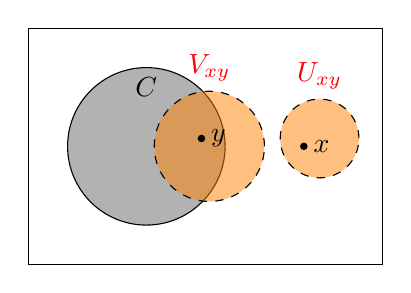
\begin{tikzpicture}
              \draw [fill=black, fill opacity=0.3] circle [radius = 1];
              \draw (-1.5, -1.5) rectangle (3, 1.5);
        
              \draw [dashed, fill=orange, fill opacity=0.5] (0.8, 0) circle [radius=0.7];
              \node [red] at (0.8, 0.7) [above] {\(V_{xy}\)};
              \draw [dashed, fill=orange, fill opacity=0.5] (2.2, 0.1) circle [radius=0.5];
              \node [red] at (2.2, 0.6) [above] {\(U_{xy}\)};
        
              \node at (0, 1) [below] {\(C\)};
              \draw[fill=black] (2,0) circle (0.04);
              \node at (2, 0) [right] {\(x\)};
        
              \draw[fill=black] (0.7, 0.1) circle (0.04);
              \node at (0.7, 0.1) [right] {\(y\)};
        
            \end{tikzpicture}
          \end{center}
        Then \(\mathscr{U}=\{V_{xy}\cap C\mid y\in C\}\) is an open cover of \(C\). Since \(C\) is compact, there exists a finite subcover \(\mathscr{V}=\{V_{xy_1}\cap C,\dots,V_{xy_n}\cap C\}\).
        
        \begin{center}
            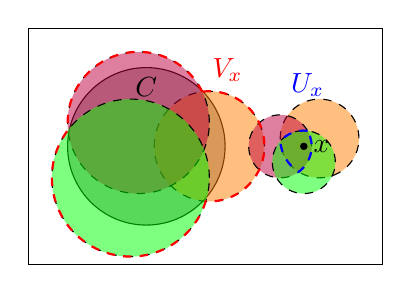
\begin{tikzpicture}
              \draw [fill=black, fill opacity=0.3]  circle [radius = 1];
              \draw (-1.5, -1.5) rectangle (3, 1.5);
        
              \draw [dashed, fill=orange, fill opacity=0.5] (0.8, 0) circle [radius=0.7];
              \draw [dashed, fill=orange, fill opacity=0.5] (2.2, 0.1) circle [radius=0.5];
        
              \draw [dashed, fill=purple, fill opacity=0.5] (-0.1, 0.3) circle [radius=0.9];
              \draw [dashed, fill=purple, fill opacity=0.5] (1.7, 0) circle [radius=0.4];
        
              \draw [dashed, fill=green, fill opacity=0.5] (-0.2, -0.4) circle [radius=1];
              \draw [dashed, fill=green, fill opacity=0.5] (2, -0.2) circle [radius=0.4];
        
              \draw [thick,red,dashed] (0.709137, 0.694078) arc (25.97:185.97:0.9) arc (142.67:342.63:1) arc (266.27:457.46:0.7) node [anchor = south west] {\(V_x\)};
        
              \draw [thick,blue,dashed] (2.04817, 0.197101) arc (83.08:138.34:0.4) arc (183.91:237.96:0.5) arc (305.94:389.51:0.4) node [above=0.3cm] {\(U_x\)};
              \node at (0, 1) [below] {\(C\)};
              \draw[fill=black] (2,0) circle (0.04);
              \node at (2, 0) [right] {\(x\)};
        
            \end{tikzpicture}
          \end{center}

        Let \(U_x=\bigcap_{i=1}^{n}U_{xy_i}\). Then \(U_x\) is open since it is a finite intersection of open sets. To show \(U_x\subset U\), note that \(V_x=\bigcup_{i=1}^{n}V_{xy_i}\supset C\) since \(\mathscr{V}=\{V_{xy_i}\cap C\}\) is an open cover. We also have \(V_x\cap U_x=\emptyset\). So \(U_x\subset U\). So done.\qed
    \end{proof}

    After relating compactness to closedness, we will relate it to boundedness. First we need to define boundedness for general metric spaces.
    \begin{defn}
        A metric space \((M,d)\) is \textit{bounded} if there exists \(L\in\mathbb{R}\) such that \(d(x,y)\le L\) for all \(x,y\in M\).
    \end{defn}
    \begin{ex}
        \(A\subset\mathbb{R}\) is bounded iff \(A\subset[-N,N]\) for some \(N\in\mathbb{R}\).
    \end{ex}
    \begin{rem}
        Note that being bounded is not a topological property. For example, \((0, 1)\cong\mathbb{R}\) but \((0,1)\) is bounded while \(\mathbb{R}\) is not. It depends on the metric \(d\), not just the topology it induces.
    \end{rem}
    \begin{prop}
        A compact metric space is bounded.
    \end{prop}
    \begin{proof}
        Pick \(x\in X\). Then \(\mathscr{U}=\{D_r(x)\mid r\in\mathbb{R}^+\}\) is an open cover of \(X\). Since \(X\) is compact, it has a finite subcover \(\{D_{r_1}(x),\dots,D_{r_n}(x)\}\). Let \(R=\max\{r_1,\dots,r_n\}\). Then \(d(x,y)<R\) for all \(y\in X\). So for all \(y,z\in X\),
        \[d(y,z)\le d(x,y)+d(x,z)<2R\,,\]
        so \(X\) is bounded.
    \end{proof}
    \begin{thm}[Heine--Borel theorem]
        \(C\subset R\) is compact if and only if \(C\) is closed and bounded.
    \end{thm}
    \begin{proof}
        Since \(\mathbb{R}\) is a metric space, it is Hausdorff and \(C\) is also a metric space.

        If \(C\) is compact, then \(C\) is closed in \(\mathbb{R}\) and is bounded by the previous two propositions.

        Conversely, if \(C\) is closed and bounded, then \(C\subset[-N,N]\) for some \(N\in\mathbb{R}\). Since \([-N,N]\cong[0,1]\) is compact, and \(C\) is closed in \([-N,N]\), \(C\) is compact.\qed
    \end{proof}
    \begin{cor}
        If \(A\subset\mathbb{R}\) is compact, \(\exists\alpha\in A\) such that \(\alpha\ge a\) for all \(a\in A\).
    \end{cor}
    \begin{proof}
        Since \(A\) is compact, it is bounded. Let \(\alpha=\sup A\). Then by definition, \(\alpha\ge a\) for all \(a\in A\). So it is enough to show that \(\alpha\in A\).

        Suppose \(\alpha\not\in A\). Then \(\alpha\in\mathbb{R}\setminus A\). Since \(A\) is compact, it is closed in \(\mathbb{R}\), so \(\mathbb{R}\setminus A\) is open. So \(\exists\epsilon>0\) such that \(D_\epsilon(\alpha)\subset\mathbb{R}\setminus A\), which implies that \(a\le\alpha-\epsilon\) for all \(a\in A\). This contradicts the assumption that \(\alpha=\sup A\). So we can conclude \(\alpha\in A\).\qed
    \end{proof}
    We call \(\alpha=\max A\) the \textit{maximum element} of \(A\).

    We have previously proved that if \(X\) is connected and \(f:X\to Y\) is continuous, then \(\im f\subset Y\) is connected. The same statement is true for compactness.

    \begin{prop}
        If \(f:X\to Y\) is continuous and \(X\) is compact, then \(\im f\subset Y\) is also compact.
    \end{prop}
    \begin{proof}
        Suppose \(\mathscr{U}=\{U_\alpha\mid\alpha\in T\}\) is an open cover of \(\im f\). Since \(U_\alpha\) is open in \(\im f\), we have \(V_\alpha=f^{-1}(U_\alpha)\) open in \(X\). If \(x\in X\) then \(f(x)\) is in \(U_\alpha\) for some \(\alpha\), so \(x\in V_\alpha\). Thus \(\mathscr{V}=\{V_\alpha\mid\alpha\in T\}\) is an open cover of \(X\).

        Since \(X\) is compact, there is a finite subcover \(\mathscr{V}'=\{V_{\alpha_1},\dots,V_{\alpha_n}\}\) of \(\mathscr{V}\). Since \(U_\alpha\subset\im f\), \(f(V_\alpha)=f(f^{-1}(U_\alpha))\subseteq U_\alpha\). So
        \[\mathscr{U}'=\{U_{\alpha_1},\dots,U_{\alpha_n}\}\]
        is a finite subcover of \(\mathscr{U}\).\qed
    \end{proof}
    \begin{thm}[Maximum value theorem]
        If \(f:X\to\mathbb{R}\) is continuous and \(X\) is compact, then \(\exists x\in X\) such that \(f(x)\ge f(y)\) for all \(y\in X\).
    \end{thm}
    \begin{proof}
        Since \(X\) is compact, \(\im f\) is compact. Let \(\alpha=\max\{\im f\}\). Then \(\alpha\in\im f\). So \(\exists x\in X\) with \(f(x)=\alpha\). Then by definition \(f(x)\ge f(y)\) for all \(y\in X\).\qed
    \end{proof}
    \begin{rem}
        A function on a compact domain is bounded and attains its bound.
    \end{rem}
    \subsection{Products and Quotients}
    \subsubsection{Products}
    Recall the product topology on \(X\cross Y\): \(U\subset X\cross Y\) is open if it is a union of sets of the form \(V\cross W\) such that \(V\subset X\), \(W\subset Y\) are open.

    The major takeaway of this section is the following theorem.
    \begin{thm}
        If \(X\) and \(Y\) are compact, then so is \(X\cross Y\).
    \end{thm}
    \begin{proof}
        First consider the special type of open cover \(\mathscr{U}\) of \(X\cross Y\) such that every \(U\in\mathscr{U}\) has the form \(U=V\cross W\), where \(V\subset X\) and \(W\subset Y\) are open. For every \((x,y)\in X\cross Y\), there is \(U_{xy}\in\mathscr{U}\) with \((x,y)\in U_{xy}\). Write
        \[U_{xy}=V_{xy}\cross W_{xy}\,,\]
        where \(V_{xy}\subset X\), \(W_{xy}\subset Y\) are open, \(x\in V_{xy}\), \(y\in W_{xy}\).

        Fix \(x\in X\). Then \(\mathscr{W}_x=\{W_{xy}\mid y\in Y\}\) is an open cover of \(Y\). Since \(Y\) is compact, there is a finite subcover \(\{W_{xy_1},\dots,W_{xy_n}\}\). Then \(V_x=\bigcap_{i=1}^{n}V_{xy_i}\) is a finite intersection of open sets. So \(V_x\) is open in \(X\). Moreover, \(\mathscr{U}_x=\{U_{xy_1},\dots,U_{xy_n}\}\) covers \(V_x\cross Y\).

        \begin{center}
            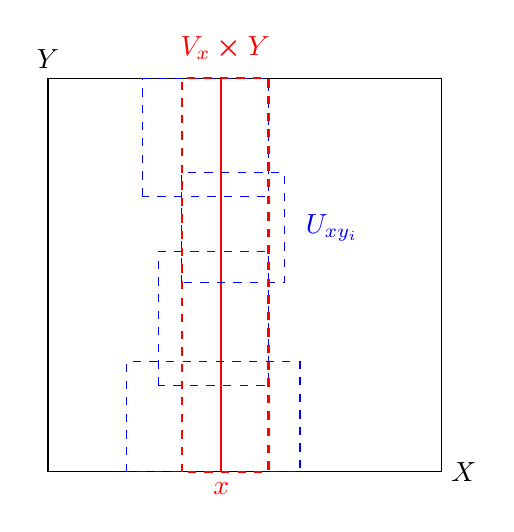
\begin{tikzpicture}
                \draw (0,0) -- (5,0) node[right]{\(X\)} -- (5,5) -- (0,5) node[above]{\(Y\)} -- (0,0);
                \draw[red,thick] (2.2,0) node[below]{\(x\)} -- (2.2,5);
                \draw[blue,dashed] (1.2,3.5) rectangle (2.8,5);
                \draw[blue,dashed] (1.7,2.4) rectangle  node[right=8mm]{\(U_{xy_i}\)}(3,3.8);
                \draw[blue,dashed] (1.4,1.1) rectangle (2.8,2.8);
                \draw[blue,dashed] (1,0) rectangle (3.2,1.4);
                \draw[red,dashed,thick] (1.7,0) rectangle node[above=2.6cm]{\(V_x\cross Y\)} (2.8,5);
            \end{tikzpicture}
        \end{center}

        Now \(\mathscr{V}=\{V_x\mid x\in X\}\) is an open cover of \(X\). Since \(X\) is compact, there is a finite subcover \(\mathscr{V}'=\{V_{x_1},\dots,V_{x_m}\}\). Then \(\mathscr{U}'=\bigcup_{i=1}^{m}\mathscr{U}_{x_i}\) is a finite subset of \(\mathscr{U}\), which covers all of \(X\cross Y\).

        In the general case, suppose \(\mathscr{U}\) is an open cover of \(X\cross Y\), For each \((x,y)\in X\cross Y\), \(\exists U_{xy}\in\mathscr{U}\) with \((x,y)\in U_{xy}\). Since \(U_{xy}\) is open, \(\exists V_{xy}\subset X\), \(W_{xy}\subset Y\) with \(V_{xy}\cross W_{xy}\subset U_{xy}\) and \(x\in V_{xy},y\in W_{xy}\).

        Then \(\mathscr{Q}=\{V_{xy}\cross W_{xy}\mid (x,y)\in X\cross Y\}\) is an open cover of \(X\cross Y\) of the type we already considered above. So it has a finite subcover \(\{V_{x_1y_1}\cross W_{x_1y_1},\dots V_{x_my_n}\cross W_{x_my_n}\}\). Now \(V_{x_iy_i}\cross W_{x_iy_i}\subset U_{x_iy_i}\). So \(\{U_{x_iy_i},\dots,U_{x_my_n}\}\) is a finite subcover of \(\mathscr{U}\).\qed
    \end{proof}
    \begin{ex}
        The unit cube \([0,1]^n=[0,1]\cross\dots\cross[0,1]\) is compact.
    \end{ex}
    \begin{cor}[Heine--Borel theorem in \(\mathbb{R}^n\)]
        \(C\subset\mathbb{R}^n\) is compact iff \(C\) is closed and bounded.
    \end{cor}
    \begin{proof}
        If \(C\) is bounded, \(C\subset[-N,N]^n\) for some \(N\in\mathbb{R}\), which is compact. The rest of the proof is the same as for \(n=1\).\qed
    \end{proof}
    \begin{cor}[Tychonoff's theorem (finite product case)]
        Finite products of compact spaces are compact.
    \end{cor}
    \begin{rem}
        This also works for arbitrary products, but the proof is much harder.
    \end{rem}
    \subsubsection{Quotients}
    \begin{prop}
        If \(X\) is compact and \(R\) is an equivalence relation on \(X\), then \(X/R\) is compact.
    \end{prop}
    \begin{proof}
        The quotient map is continuous and surjective, so its image is compact.\qed
    \end{proof}

    \begin{thm}[Topological inverse function theorem]
        Suppose \(f:X\to Y\) is a continuous bijection. If \(X\) is compact and \(Y\) is Hausdorff, then \(f\) is a homeomorphism.
    \end{thm}
    \begin{proof}
        We show that \(f^{-1}\) is continuous. To do this, it suffices to show \((f^{-1})^{-1}(C)\) is closed in \(Y\) whenever \(C\) is closed in \(X\). By hypothesis, \(f\) is a bijection, so \((f^{-1})^{-1}(C)=f(C)\). Suppose \(C\) is closed in \(X\). Since \(X\) is compact, \(C\) is compact. Since \(f\) is continuous, \(f(C)=\im f|_C\) is compact. Since \(Y\) is Hausdorff and \(f(C)\subset Y\) is compact, \(f(C)\) is closed as required.\qed
    \end{proof}

    We will apply this to quotients.

    Recall that if \(R\) is an equivalence relation on \(X\), \(q:X\to X/R\) is continuous if and only if \(f:X\to Y\) is continuous, where \(f\equiv \tilde{f}\circ q\) is defined such that \(xRy\implies f(x)=f(y)\).

    \begin{cor}
        Suppose \(\tilde{f}:X/R\to Y\) is a bijection, \(X\) is compact, \(Y\) is Hausdorff, and \(\tilde{f}\circ q\) is continuous, then \(\tilde{f}\) is a homeomorphism.
    \end{cor}
    \begin{proof}
        Since \(X\) is compact and \(q:X\to X/R\) is continuous, \(\im q\subset X/R\) is compact. Since \(\tilde{f}\circ q\) is continuous, \(\tilde{f}\) is continuous, so we can apply the above proposition.
    \end{proof}
    \begin{ex}
        Let \(X=D^2\) and \(A=S^1\subset X\). Then
        \begin{align*}
            \tilde{f}:X/A&\to S^2\\
            (r,\theta)&\mapsto(1,\pi r,\theta)
        \end{align*}
        in spherical coordinates is a homeomorphism.

        We can check that \(\tilde{f}\) is a continuous bijection and \(D^2\) is compact. So \(D^2/S^1\cong S^2\).
    \end{ex}
    \subsection{Sequential Compactness}
    The other definition of compactness is sequential compactness. We will not do much with it, but only prove that it is the same as compactness for metric spaces.

    \begin{defn}
        A topological space \(X\) is \textit{sequentially compact} if every sequence \(x_n\in X\) has a convergent subsequence.
    \end{defn}
    \begin{ex}
        Any closed and bounded subset of \(\mathbb{R}^n\) is sequentially compact by Bolzano--Weierstrass theorem.
    \end{ex}

    \begin{lem}
        Let \(x_n\) be a sequence in a metric space \((M,d)\) and \(x\in M\). Then \(x_n\) has a subsequence converging to \(x\) if and only if for every \(\epsilon>0\), \(x_n\in D_\epsilon(x)\) for infinitely many \(n\).
    \end{lem}
    \begin{proofskip}
        \begin{itemize}
            \item[(\(\Rightarrow\))] If \(x_{n_i}\to x\), then for every \(\epsilon>0\), we can find \(I\in\mathbb{N}\) such that \(i>I\) implies \(x_{n_i}\in D_\epsilon(x)\).
            \item[(\(\Leftarrow\))] Now suppose for every \(\epsilon>0\), there are infinitely many \(x_n\in D_\epsilon(x)\). We will construct a sequence \(x_{n_i}\) inductively. Take \(n_0=0\). Suppose we have defined \(x_{n_0},\dots,x_{n_{i-1}}\). By hypothesis \(x_n\in D_{1/i}(x)\) for infinitely many \(n\). Take \(n_i\) to the smallest such \(n\) with \(n_i>n_{i-1}\). Then \(d(x_{n_i},x)<1/i\) implies that \(x_{n_i}\to x\).\qed
        \end{itemize}
    \end{proofskip}

    \begin{defn}
        Let \((M,d)\) be a metric space. For \(\epsilon>0\) and \(F\subset M\). We say \(F\) is an \textit{\(\epsilon\)-net} for \(M\) if \(\forall x\in M\), \(\exists y\in F\) such that \(d(x,y)\le\epsilon\). That is,
        \[M=\bigcup_{y\in F}B_\epsilon(y)\,.\]

        We say \(M\) is \textit{totally bounded} if for any \(\epsilon>0\), there is a finite \(\epsilon\)-net for \(M\).
    \end{defn}
    \begin{ex}
        For \(\epsilon>0\), take \(n\) such that \(1/n<\epsilon\). Then
        \[\qty{\frac{1}{n},\frac{2}{n},\dots,\frac{n-1}{n}}\]
        is an \(\epsilon\)-net for \((0,1)\).
    \end{ex}

    Note that any compact space is totally bounded, but the converse is not true. The \((0,1)\) above is an example. The only thing missing here is completeness.

    \begin{defn}
        For a non-empty set \(A\subset M\), the \textit{diameter} of \(A\) is
        \[\diam A\coloneqq\sup_{x,y\in A}d(x,y)\,.\]        
    \end{defn}
    Clearly, the diameter of a set is finite if and only if it is bounded.

    \begin{thm}
        For a metric space, the following are equivalent:
        \begin{enumerate}[label=(\roman*),topsep=0pt]
            \item \(M\) is compact.
            \item \(M\) is sequentially compact.
            \item \(M\) is totally bounded and complete.
        \end{enumerate}
    \end{thm}
    \begin{proofskip}
        \begin{itemize}[topsep=0pt]
            \item (i) \(\Rightarrow\) (ii). Let \(x_n\) be a sequence in \(M\), so for \(n\in\mathbb{N}\), let \(A_n=\{x_k\mid k>N\}\). Note that the limit of any convergent subsequence, if it exists, is in the intersection \(\bigcap_{n\in\mathbb{N}}\bar{A}_n\). We first show that it is non-empty. Assume it is empty, then
            \[\bigcup_{n\in\mathbb{N}}M\setminus\bar{A}_n=M\,.\]
            Each \(M\setminus\bar{A}_n\) is open, so it is an open cover of \(M\). By the compactness of \(M\), it has a finite subcover, so there is some \(N\in\mathbb{N}\) such that \(\bigcup_{n\le N}M\setminus\bar{A}_n=M\). But \(\{A_n\}\) is decreasing, so necessarily \(M\setminus\bar{A}_N=M\), then \(\bar{A}_N=\emptyset\). Contradiction.

            Now let \(x\in\bigcap_{n\in\mathbb{N}}\bar{A}_n\), and we want to show the existence of a subsequence converging to \(x\). First, \(x\in\bar{A}_1\), so \(D_1(x)\cap A_1\ne\emptyset\). Hence there exists \(k_1>1\) such that \(d(x_{k_1},x)<1\). Now since \(x\in\bar{A}_{k_1}\), \(D_{1/2}(x)\cap A_{k_1}\ne\emptyset\), there exists \(k_2>k_1\) such that \(d(x_{k_2},x)<1/2\). Inductively, we can find \(k_1<k_2<\dots\) such that \(d(x_{k_n},x)<\frac{1}{n}\) for all \(n\in\mathbb{N}\). Hence \(x_{k_n}\to x\). 
            \item (ii) \(\Rightarrow\) (iii). \(M\) is complete since a Cauchy sequence with a convergent subsequence is convergent. To see it is totally bounded, assume it is not, then there is some \(\epsilon>0\) such that every \(\epsilon\)-net is infinite. Pick any \(x_1\in M\), and once we have already picked \(x_1,\dots,x_n\), we pick \(x_{n+1}\not\in\bigcup_{k=1}^{n}B_\epsilon(x_k)\). This is always valid since otherwise \(M\) would have a finite \(\epsilon\)-net. But then the sequence \(x_n\) cannot have any Cauchy subsequence, so it has no converging subsequence.
            \item (iii) \(\Rightarrow\) (i). Assume such an \(M\) is not compact, so there is an open cover \(\mathscr{U}\) without any finite subcover. We say \(A\subset M\) is ``bad'' if there is no finite subcover of \(A\) in \(\mathscr{U}\). So, for example, \(M\subset M\) is bad while \(\emptyset\subset M\) is not. Note if \(A=\cup_{i=1}^{n}B_i\) is bad, then there is some \(i\) such that \(B_i\) is bad.
            
            Next, we want to show that if \(A\) is bad and \(\epsilon>0\), then \(\exists B\subset A\) such that \(B\) is bad and \(\diam B<\epsilon\). Indeed, since \(M\) is totally bounded, we have a finite \(\epsilon/2\)-net \(F\). Then \(M=\bigcup_{x\in F}B_{\epsilon/2}(x)\), and hence \(A=\bigcup_{x\in F}(B_{\epsilon/2}(x)\cap A)\). Since \(A\) is bad, there is some \(x\in F\) such that \(B_{\epsilon/2}(x)\cap A\) is bad, which has a diameter less than \(\epsilon\). From this we can construct a sequence \(M\supset A_1\supset A_2\supset\dots\) such that \(A_n\) is bad for any \(n\) and \(\diam A_n<1/n\). Picking \(x_n\in A_n\) gives a Cauchy sequence \(x_n\) which converges to \(x\in M\) by completeness. There must be some \(U\subset\mathscr{U}\) open that contains \(x\), and it necessarily covers \(A_n\) when \(n\) is large enough. Then \(A_n\) is not bad. Contradiction.\qed
        \end{itemize}
    \end{proofskip}\
    \begin{rems}
        \begin{enumerate}[label=(\roman*),topsep=0pt]
            \item This is a new proof of Bolzano--Weierstrass theorem. This also proves the Tychonoff's theorem.
            \item Sadly, the equivalence of sequential compactness and compactness fails in both directions for a general topological space.
        \end{enumerate}
    \end{rems}

    \newpage
    \section{Differentiation}
    \subsection{Differentiation}
    Recall that a function \(f:\mathbb{R}\to\mathbb{R}\) is differentiable at \(a\) if
    \[\lim_{h\to 0}\frac{f(a+h)-f(a)}{h}\]
    exists. So let
    \[\epsilon(h)=\frac{f(a+h)-f(a)}{h}-f'(a)\,,\]
    then \(f(a+h)=f(a)+f'(a)h+\epsilon(h)h\) and \(\epsilon\to 0\) as \(h\to 0\). We can think of this as \(\epsilon(0)=0\) and \(\epsilon\) is continuous at \(0\). We want to use this to define differentiation in higher dimensions. Consider functions from \(\mathbb{R}^m\) to \(\mathbb{R}^n\), where \(m,n\in\mathbb{N}\).
    \begin{defn}
        \(L(\mathbb{R}^m,\mathbb{R}^n)\) denotes the set of linear maps from \(\mathbb{R}^m\) to \(\mathbb{R}^n\).
    \end{defn}
    \begin{defn}
        Given \(m,n\in\mathbb{N}\) and an open set \(U\subset\mathbb{R}^m\), a function \(f:U\to\mathbb{R}^n\) and \(a\in U\). We say \(f\) is \textit{differentiable} at \(a\) if there is a linear map \(T:\mathbb{R}^m\to\mathbb{R}^n\) and a function \(\epsilon:\{h\in\mathbb{R}^m\mid a+h\in U\}\to\mathbb{R}^n\) such that
        \[f(a+h)=f(a)+T(h)+\epsilon(h)\norm{h}\,,\]
        where \(\epsilon\to 0\) as \(h\to 0\) (or equivalently \(\epsilon(0)=0\) and \(\epsilon\) is continuous at \(0\)).
    \end{defn}
    \begin{rem}
        \[\epsilon(h)=\left\{\begin{aligned}
            &\;0 && \text{if }h=0\,,\\
            &\;\frac{f(a+h)-f(a)-T(h)}{\norm{h}} && \text{if }h\ne 0,a+h\in U\,.
        \end{aligned}\right.\]
        Since \(U\) is open, \(\exists r>0\) such that \(D_r(a)\subset U\), so \(D_r(a)\subset\Dom\epsilon\). Note that our condition on \(\epsilon\) is equivalent to saying \(\epsilon(h)\norm{h}=o(\norm{h})\) as \(h\to 0\).
        
        Alternatively, we may write
        \[\lim_{h\to 0}\frac{f(a+h)-f(a)-T(h)}{\norm{h}}=0\,.\]
    \end{rem}

    Next, we observe that such \(T\), if it exists, is unique. If both \(T,S\) satisfy our condition, then \((S(h)-T(h))/\norm{h}\to 0\) as \(h\to 0\), so by choosing \(h=x/n\) for \(n\in\mathbb{N}\) we have \(S=T\).

    \begin{defn}
        This unique \(T\) is called the \textit{derivative} of \(f\) at \(a\), usually denoted by \(f'(a)\), \(Df(a)\) or \(Df|_a\), such that
        \[f(a+h)=f(a)+f'(a)h+o(\norm{h})\,.\]
    \end{defn}
    \begin{defn}
        We say \(f\) is \textit{differentiable} on \(U\) if it is differentiable at \(a\) for every \(a\in U\). The \textit{derivative} of \(f\) on \(U\) is the map
        \begin{align*}
            f':U&\to L(\mathbb{R}^m,\mathbb{R}^n)\\
            x&\mapsto f'(x)
        \end{align*}
    \end{defn}
    \begin{exs}
        \begin{enumerate}[label=(\roman*),topsep=0pt]
            \item Constant functions are differentiable. We can take \(f'(a)=0\in L(\mathbb{R}^m,\mathbb{R}^n)\).
            \item Every linear map \(f\) is differentiable. Let \(f(x)=T(x)\) for some \(T\in L(\mathbb{R}^m,\mathbb{R}^n)\). Then
            \[f(a+h)=f(a)+f(h)+0\]
            so \(f\) is differentiable at \(a\) with a derivative \(T\).
            \item Take \(f:\mathbb{R}^n\to\mathbb{R}\) by \(f(x)=\norm{x}^2\). Then
            \begin{align*}
                f(a+h)&=\norm{a+h}^2\\
                &=\norm{a}^2+2\braket{a}{h}+\norm{h}^2\\
                &=f(a)+2\braket{a}{h}+o(\norm{h})\,,
            \end{align*}
            so \(f'(a)(h)=2\braket{a}{h}\).
        \end{enumerate}
    \end{exs}
    \begin{prop}[Differentiable functions are continuous]
        Let \(U\subset\mathbb{R}^m\) and \(a\in U\). If \(f:U\to\mathbb{R}^n\) is differentiable at \(a\), then \(f\) is continuous at \(a\).
    \end{prop}
    \begin{proof}
        If \(f\) is differentiable, then as \(h\to 0\), we have
        \[f(a+h)-f(a)-f'(a)(h)\to 0\,.\]
        Since \(f'(a)(h)\to 0\) as well, we must have \(f(a+h)\to f(a)\).\qed
    \end{proof}
    \subsection{Operator Norm}
    So far, we have only looked at derivatives at a single point. We haven't yet discussed much about the derivative at a neighbourhood or the whole space. We might also want to ask if the derivative is continuous or bounded. This is not a straightforward question as we need to define these notions for functions whose values are linear maps. In particular, we want to understand the map \(Df:B_r(a)\to L(\mathbb{R}^m,\mathbb{R}^n)\). To do so, we need a metric on the space \(L(\mathbb{R}^m,\mathbb{R}^n)\). We will do this by defining a norm.

    \(L(\mathbb{R}^m,\mathbb{R}^n)\) is a vector space over \(\mathbb{R}\) with addition and scalar multiplication defined pointwise. In fact, it is a subspace of \(C(\mathbb{R}^m,\mathbb{R}^n)\). To prove this, we will need to show that all linear maps are continuous.
    \begin{lem}
        Linear maps in \(L(\mathbb{R}^m,\mathbb{R}^n)\) are Lipschitz and hence continuous.
    \end{lem}
    \begin{proof}
        Let \(\{e_i\}\) be the standard basis for \(\mathbb{R}^m\) and \(x=\sum_i x_i e_i\). By Cauchy--Schwarz,
        \begin{align*}
            \norm{Tx}&\le\sum_{i=1}^{m}\abs{x_i}\norm{Te_i}\\
            &\le\sqrt{\sum_{i=1}^{m}\abs{x_i}^2}\sqrt{\sum_{i=1}^{m}\norm{Te_i}^2}\\
            &=\norm{x}\sqrt{\sum_{i=1}^{m}\norm{Te_i}^2}\,.
        \end{align*}\qed
    \end{proof}

    We can use this fact to define the norm of linear maps. \(L(\mathbb{R}^m,\mathbb{R}^n)\) is isomorphic to \(\mathbb{R}^{mn}\), both algebraically and topologically, since it is isomorphic to \(M_{n\times m}\), the space of \(n\times m\) real matrices. It does not really matter which norm we pick as they are all Lipschitz equivalent. We will introduce two of them.

    \subsubsection{Sup Norm}
    \begin{defn}
        The \textit{sup norm} on \(L(\mathbb{R}^m,\mathbb{R}^n)\) is defined by
        \[\norm{A}=\sup_{x\in\mathbb{R}^m,\norm{x}=1}\norm{Ax}\,.\]
    \end{defn}
    Thus, \(L(\mathbb{R}^m,\mathbb{R}^n)\) becomes a metric space with the metric \(d(S,T)=\norm{S-T}\).
    \begin{propskip}
        \begin{enumerate}[label=(\roman*),topsep=0pt]
            \item \(\norm{A}\) is finite.
            \item \(\norm{\;\vdot\;}\) is indeed a norm on \(L(\mathbb{R}^m,\mathbb{R}^n)\).
            \item
            \[\norm{A}=\sup_{x\in\mathbb{R}^m\setminus\{0\}}\frac{\norm{Ax}}{\norm{x}}\,.\]
            \item \(\norm{Ax}\le\norm{A}\norm{x}\) for all \(x\in\mathbb{R}^m\).
            \item Let \(A\in L(\mathbb{R}^m,\mathbb{R}^n)\), \(B\in L(\mathbb{R}^n,\mathbb{R}^p)\). Then \(BA=B\circ A\in L(\mathbb{R}^m,\mathbb{R}^p)\) and
            \[\norm{BA}\le\norm{B}\norm{A}\,.\]
        \end{enumerate}
    \end{propskip}
    \begin{proofskip}
        \begin{enumerate}[label=(\roman*),topsep=0pt]
            \item This is true because \(A\) is continuous and \(\{x\in\mathbb{R}^m\mid\norm{x}=1\}\) is compact.
            \item The only non-trivial part is the triangle inequality. We have
            \begin{align*}
                \norm{A+B}&=\sup_{\norm{x}=1}\norm{Ax+Bx}\\
                &\le\sup_{\norm{x}=1}(\norm{Ax}+\norm{Bx})\\
                &\le\sup_{\norm{x}=1}\norm{Ax}+\sup_{\norm{x}=1}\norm{Bx}\\
                &=\norm{A}+\norm{B}\,.
            \end{align*}
            \item This follows from the linearity of \(A\), and the fact that for any \(x\in\mathbb{R}^m\), we have
            \[\norm{\frac{x}{\norm{x}}}=1\,.\]
            \item Immediate from above.
            \item
            \[\norm{BA}=\sup_{x\in\mathbb{R}^m\setminus\{0\}}\frac{\norm{BAx}}{\norm{x}}\le\sup_{x\in\mathbb{R}^m\setminus\{0\}}\frac{\norm{B}\norm{Ax}}{\norm{x}}=\norm{B}\norm{A}\,.\]
        \end{enumerate}\qed
    \end{proofskip}
    For certain easy cases, we have a straightforward expression for the operator norm.
    \begin{propskip}
        \begin{enumerate}[label=(\roman*),topsep=0pt]
            \item If \(A\in L(\mathbb{R},\mathbb{R}^n)\), then \(A\) can be written as \(Ax=xa\) for some \(a\in\mathbb{R}^n\). Moreover, \(\norm{A}=\norm{a}\), where the second norm is the Euclidean norm in \(\mathbb{R}^n\).
            \item If \(A\in L(\mathbb{R}^m,\mathbb{R})\), then \(Ax=x\vdot a\) for some fixed \(a\in\mathbb{R}^m\). Also, \(\norm{A}=\norm{a}\).
        \end{enumerate}
    \end{propskip}
    \begin{proofskip}
        \begin{enumerate}[label=(\roman*),topsep=0pt]
            \item Set \(A(1)=a\). Then by linearity, we get \(Ax=xA(1)=xa\). Then we have
            \[\norm{Ax}=\abs{x}\norm{a}\,.\]
            \item Let \(\{e_i\}\) be the standard basis of \(\mathbb{R}^m\). Let \(a_i=Ae_i\) and \(a=\sum_i a_ie_i\). The rest follows by linearity.\qed
        \end{enumerate}
    \end{proofskip}

    \subsubsection{Euclidean Norm}
    Let \(\{e_i\}_{i=1}^{m}\) be the standard basis of \(\mathbb{R}^m\) and let \(\{e_j'\}_{j=1}^{n}\) be the standard basis of \(\mathbb{R}^n\). Then \(T\in L(\mathbb{R}^m,\mathbb{R}^n)\) is identified with a \(n\times m\) matrix \(\mathsf{T}\), where \(T_{ji}=\braket{Te_i}{e_j'}\). We can therefore view \(L(\mathbb{R}^m,\mathbb{R}^n)\) as the \(mn\)-dimensional vector space \(\mathbb{R}^{mn}\), which can be equipped with an Euclidean norm.
    \begin{defn}
        The \textit{Euclidean norm} on \(L(\mathbb{R}^m,\mathbb{R}^n)\) is defined by
        \[\norm{T}=\sqrt{\sum_{i=1}^{m}\sum_{j=1}^{n}T_{ji}^2}=\sqrt{\sum_{i=1}^{m}\norm{Te_i}^2}\,,\]
        where \(Te_i\) is the \(i\)-th column of \(\mathsf{T}\). 
    \end{defn}
    Again, we have the metric \(d(S,T)=\norm{S-T}\) on \(L(\mathbb{R}^m,\mathbb{R}^n)\).

    \begin{lemskip}
        \begin{enumerate}[label=(\roman*),topsep=0pt]
            \item Given a linear map \(T\), for every \(x\in\mathbb{R}^m\), we have \(\norm{Tx}\le\norm{T}\norm{x}\).
            \item For \(S\in L(\mathbb{R}^m,\mathbb{R}^n)\), \(T\in L(\mathbb{R}^n,\mathbb{R}^p)\), \(\norm{TS}\le\norm{T}\norm{S}\).
        \end{enumerate}
    \end{lemskip}
    \begin{proofskip}
        \begin{enumerate}[label=(\roman*),topsep=0pt]
            \item Let \(x=\sum_i x_i e_i\), then
            \begin{align*}
                \norm{Tx}\le\sqrt{\sum_{i=1}^{m}\abs{x_i}^2}\sqrt{\sum_{i=1}^{m}\norm{Te_i}^2}=\norm{x}\norm{T}
            \end{align*}
            by Cauchy--Schwarz, as shown before.
            \item
            \[\norm{TS}=\sqrt{\sum_{i=1}^{m}\norm{TSe_i}^2}\le\sqrt{\sum_{i=1}^{m}\norm{T}^2\norm{Se_i}^2}=\norm{T}\norm{S}\,.\]\qed
        \end{enumerate}
    \end{proofskip}

    As these two definitions of the norm on \(L(\mathbb{R}^m,\mathbb{R}^n)\) are equivalent, we will not distinguish them in the future. The notation \(\norm{T}\) may refer to either of them.

    \begin{ex}
        Any bilinear map \(f:\mathbb{R}^m\cross\mathbb{R}^n\to\mathbb{R}^p\) is differentiable. We have
            \[f((a,b)+(h,k))=f((a+h,b+k))=f(a,b)+f(a,k)+f(h,b)+f(h,k)\,.\]
            Note that \(f(a,k)+f(h,b)\) is linear in \((h,k)\), therefore it remains to check \(f(h,k)=o(\norm{(h,k)})\). Indeed,
            \begin{align*}
                \norm{f(h,k)}&=\norm{f\qty(\sum_{i=1}^{m}h_ie_i,\sum_{j=1}^{n}k_je_j)}\\
                &\le\sum_{i,j}\abs{h_i}\abs{k_j}\norm{f(e_i,e_j)}\\
                &\le\norm{(h,k)}^2\sum_{i,j}\norm{f(e_i,e_j)}\\
                &=O(\norm{(h,k)}^2)=o(\norm{(h,k)})\,.
            \end{align*}
            Therefore,
            \[f'(a,b)(h,k)=f(a,k)+f(h,b)\,.\]
            \item Let \(M_n=L(\mathbb{R}^n,\mathbb{R}^n)\) be the collection of all \(n\times n\) real matrices. Consider \(f:M_n\to M_n\), \(A\mapsto A^2\). It has
            \[f(A+H)=A^2+AH+HA+H^2=f(A)+AH+HA+o(\norm{H})\,.\]
            So \(f'(A)(H)=AH+HA\).
    \end{ex}
    \begin{prop}[Chain rule]
        Consider open sets \(U\subset\mathbb{R}^m\), \(V\subset\mathbb{R}^n\) and functions \(f:U\to\mathbb{R}^n\), \(g:V\to\mathbb{R}^p\) such that \(f(U)\subset V\). If \(f\) is differentiable at \(a\) and \(g\) is differentiable at \(f(a)\), then \(g\circ f\) is differentiable at \(a\) and
        \[(g\circ f)'(a)=g'(f(a))f'(a)\,.\]
    \end{prop}
    \begin{proof}
        Let \(A=f'(a)\) and \(B=g'(f(a))\). By the differentiability of \(f\), we know
        \[\begin{cases*}
            f(a+h)=f(a)+Ah+o(\norm{h})\\
            g(f(a)+k)=g(f(a))+Bk+o(\norm{k})\,.
        \end{cases*}\]
        Now we have
        \begin{align*}
            g\circ f(a+h)&=g(f(a)+\underbrace{Ah+o(\norm{h})}_{k})\\
            &=g(f(a))+B(Ah+o(\norm{h}))+o(Ah+o(\norm{h}))\\
            &=g\circ f(a)+BAh+B(o(\norm{h}))+o(Ah+o(\norm{h}))\,.
        \end{align*}
        We only have to show that the last two terms are \(o(\norm{h})\). This is true since
        \[B(o(\norm{h}))\le\norm{B}\norm{o(\norm{h})}=o(\norm{h})\,,\]
        and for sufficiently small \(h\),
        \[\norm{Ah+o(\norm{h})}\le\norm{A}\norm{h}+\norm{o(\norm{h})}\le(\norm{A}+1)\norm{h}\,,\]
        so \(o(Ah+o(\norm{h}))\) is \(o(\norm{h})\) as well. Hence
        \[g\circ f(a+h)=g\circ f(a)+BAh+o(\norm{h})\,.\]\qed
    \end{proof}
    \begin{prop}
        Let \(U\subset\mathbb{R}^m\) be open. \(f:U\to\mathbb{R}^n\) is differentiable at \(a\in U\) if and only if each component \(f_j=\pi_j\circ f\) is differentiable at \(a\). Also,
        \[f'(a)(h)=\sum_{j=1}^{n}f'_j(a)(h)e'_j\,.\]
    \end{prop}
    \begin{proofskip}
        \begin{itemize}
            \item[(\(\Rightarrow\))] \(\pi_j(x)=\braket{x}{e'_j}\) is linear hence differentiable. Trivial by chain rule.
            \item[(\(\Leftarrow\))]
            \begin{align*}
                f(a+h)&=\sum_{j=1}^{n}f_j(a+h)e'_j\\
                &=\sum_{j=1}^{n}(f_j(a)+f_j'(a)(h)+\epsilon_j(h)\norm{h})e'_j\\
                &=f(a)+\qty(\sum_{j=1}^{n}f'_j(a)(h)e'_j)+\qty(\sum_{j=1}^{n}\epsilon_j(h)e'_j)\norm{h}\,,
            \end{align*}
            where the last term is \(o(\norm{h})\).\qed
        \end{itemize}
    \end{proofskip}
    \begin{prop}[Linearity and product rule]
        Let \(f,g:U\to\mathbb{R}^n\), \(\phi:U\to\mathbb{R}\), where \(U\subset\mathbb{R}^m\) is open. If \(f,g,\phi\) are differentiable at \(a\in U\), then so are \(f+g\) and \(\phi f\), and
        \[(f+g)'(a)=f'(a)+g'(a)\,,\]
        \[(\phi f)'(a)(h)=\phi'(a)(h)f(a)+\phi(a)f'(a)(h)\,.\]
    \end{prop}
    \begin{proof}
        Have
        \[f(a+h)=f(a)+f'(a)(h)+o(\norm{h})\,,\]
        \[g(a+h)=g(a)+g'(a)(h)+o(\norm{h})\,,\]
        \[\phi(a+h)=\phi(a)+\phi'(a)(h)+o(\norm{h})\,.\]
        Hence
        \[(f+g)(a+h)=(f+g)(a)+(f'(a)+g'(a))(h)+o(\norm{h})\,.\]

        We can do the same thing to derive the product rule, but here we will provide an alternative proof. Let \(F:U\to\mathbb{R}\cross\mathbb{R}^n=\mathbb{R}^{n+1}\) by \(x\mapsto(\phi(x),f(x))\), and \(G:\mathbb{R}\cross\mathbb{R}^n\to\mathbb{R}^n\) by \((a,x)\mapsto ax\). \(F\) is differentiable by the previous proposition, and \(G\) is differentiable since it is bilinear. Hence \(\phi f=G\circ F\) is differentiable and we can obtain the form of the derivative by chain rule.\qed
    \end{proof}
    
    \subsection{Directional and Partial Derivatives}
    While the definition of the derivative is good, it is purely existential. This is unlike the definition of differentiability of real functions, where we are asked to compute an explicit limit if the limit exists, that's the derivative. If not, it is not differentiable. In the higher-dimensional world, this is not the case. We have completely no idea where to find the derivative, even if we know it exists. So we would like an explicit formula for it.

    The idea is to look at specific directions instead of finding the general derivative. As always, let \(f:U\to\mathbb{R}^n\) be differentiable at \(a\in U\). Fix some non-zero \(u\in\mathbb{R}^m\), take \(h=tu\) with \(t\in\mathbb{R}\). Differentiability tells
    \begin{align*}
        &\lim_{t\to0}\frac{f(a+tu)-f(a)-f'(a)(tu)}{\norm{tu}}=0\\
        \iff&\lim_{t\to0}\frac{f(a+tu)-f(a)-tf'(a)(u)}{t}=0\\
        \iff&f'(a)(u)=\lim_{t\to 0}\frac{f(a+tu)-f(a)}{t}\,.
    \end{align*}
    We derived this assuming \(u\ne 0\), but this is trivially true for \(u=0\). So this is valid for all \(u\in\mathbb{R}^m\).

    This is of the same form as the usual derivative, and it is usually not too difficult to compute this limit. Note, however, that this says if the derivative exists, then the limit above is related to the derivative as above. However, even if the limit exists for all \(u\), we still cannot conclude that the derivative exists. Regardless, even if the derivative does not exist, this limit is still often a useful notion.
    \begin{defn}
        Let \(f:U\to\mathbb{R}^n\), where \(U\subset\mathbb{R}^m\) is open. For \(u\in\mathbb{R}^m\) and \(a\in U\), the \textit{directional derivative} of \(f\) at \(a\) in the direction of \(u\) is the limit
        \[D_uf(a)\coloneqq\lim_{t\to 0}\frac{f(a+tu)-f(a)}{t}\,.\]
    \end{defn}
    
    By definition, we have
    \[D_uf(a)=\left.\dv{t}\right|_{t=0}f(a+tu)\,.\]
    
    Often, it is convenient to focus on the special cases where \(u=e_i\), a member of the standard basis for \(\mathbb{R}^m\). This is known as the partial derivative. By convention, this is defined for real-valued functions only, but the same definition works for any \(\mathbb{R}^n\)-valued function.
    
    \begin{defn}
        The \text{\(j\)-th partial derivative} of \(f:U\to\mathbb{R}\) at \(a\in U\subset\mathbb{R}^m\) is
        \[D_{e_j}f(a)=\lim_{t\to 0}\frac{f(a+te_j)-f(a)}{t}\]
        if the limit exists. This is often written
        \[D_{e_j}f(a)=D_jf(a)=\pdv{f}{x_j}(a)\,.\]
    \end{defn}

    Note that these definitions do not require differentiability of \(f\) at \(a\). We will see some examples shortly. Before that, we first establish some elementary properties of differentiable functions.

    \begin{prop}
        Let \(U\subset\mathbb{R}^m\) be open and \(a\in U\).
        \begin{enumerate}[label=(\roman*),topsep=0pt]
            \item If \(f:U\to\mathbb{R}^n\) is differentiable at \(a\), then the directional derivative \(D_u f(a)\) exists for any \(u\in\mathbb{R}^m\), and
            \[D_uf(a)=Df(a)u\,.\]
            \item If \(f=(f_1,\dots,f_n):U\to\mathbb{R}^n\) is differentiable at \(a\), then all partial derivatives \(D_jf_i(a)\) exist for all \(i=1,\dots,n\), \(j=1,\dots,m\), and are given by
            \[D_jf_i(a)=Df_i(a)e_j\,.\]
            \item If \(\mathsf{A}\) is the matrix representing \(Df(a)\) with respect to the basis for \(\mathbb{R}^m\) and \(\mathbb{R}^n\), i.e. for any \(h\in\mathbb{R}^m\),
            \[Df(a)h=\mathsf{A}h\,.\]
            Then \(A\) is given by
            \[A_{ij}=\braket{Df(a)e_j}{b_i}=D_jf_i(a)\,,\]
            where \(\{e_1,\dots,e_m\}\) and \(\{b_1,\dots,b_n\}\) are the standard basis of \(\mathbb{R}^m\) and \(\mathbb{R}^n\) respectively.
        \end{enumerate}
    \end{prop}
    \begin{rem}
        This is often expressed in the form
        \[f'(a)(h)=\sum_{i=1}^{m}h_iD_if(a)\,.\]
    \end{rem}
    \begin{proofskip}
        \begin{enumerate}[label=(\roman*),topsep=0pt]
            \item Obvious from above discussion.
            \item Obvious from above discussion.
            \item This follows from the general result for linear maps: for any linear map represented by a \(m\times n\) matrix \((A_{ij})\), we have
            \[A_{ij}=\braket{\mathsf{A}e_j}{b}\,.\]
            Apply this with \(\mathsf{A}=Df(a)\) and note that for any \(h\in\mathbb{R}^n\),
            \[Df(a)(h)=(Df_1(a)h,\dots,Df_m(a)h)\,.\]
            So done.\qed
        \end{enumerate}
    \end{proofskip}
    \begin{defn}
        Let \(f\) be differentiable at \(a\). The \textit{Jacobian matrix} of \(f\) at \(a\), denoted \(J_f(a)\) is the matrix of \(f'(a)\) with respect to the standard bases
        \[(J_f(a))_{ji}=\braket{D_if(a)}{e'_j}=\pi_j(D_if(a))=D_if_j(a)=\pdv{f_j}{x_i}\,.\]
    \end{defn}
    The above says differentiability at a point implies the existence of all directional derivatives, which in turn implies the existence of all partial derivatives. The converse implication does not hold in either of these.
    \begin{ex}
        Define
        \begin{align*}
            f:\mathbb{R}^2&\to\mathbb{R}\\
            (x,y)&\mapsto\left\{\begin{aligned}
                \;0 & \qquad xy=0\\
                \;1 & \qquad xy\ne 0\,.
            \end{aligned}\right.
        \end{align*}
        Then the partial derivatives at \((0,0)\) are
        \[\pdv{f}{x}(0,0)=\pdv{f}{y}(0,0)=0\,.\]
        In other directions, say \(u=(1,1)\), we have
        \[D_{u}f(0,0)=\lim_{t\to 0}\frac{f((0,0)+tu)-f(0,0)}{t}=\lim_{t\to 0}\frac{1}{t}\]
        which diverges. So the directional derivative does not exist.
    \end{ex}
    \begin{ex}
        Define
        \begin{align*}
            f:\mathbb{R}^2&\to\mathbb{R}\\
            (x,y)&\mapsto\left\{\begin{aligned}
                &\;\frac{x^3}{y} && \quad y\ne0\\
                &\;0 && \quad y=0\,.
            \end{aligned}\right.
        \end{align*}
        Then for \(u=(u_1,u_2)\ne 0\) and \(t\ne 0\), we can compute
        \[\frac{f((0,0)+tu)-f(0,0)}{t}=\left\{\begin{aligned}
            &\;\frac{tu_1^3}{u_2} &&\quad u_2\ne 0\\
            &\;0 &&\quad u_2=0\,.
        \end{aligned}\right.\]
        So
        \[D_uf(0,0)=\lim_{t\to 0}\frac{f((0,0)+tu)-f(0,0)}{t}=0\,,\]
        and the directional derivatives exist in all directions. However, the function is not differentiable at \((0,0)\), since it is even not continuous there. 
    \end{ex}
    \begin{ex}
        Define
        \begin{align*}
            f:\mathbb{R}^2&\to\mathbb{R}\\
            (x,y)&\mapsto\left\{\begin{aligned}
                &\;\frac{x^3}{x^2+y^2} && \quad (x,y)\ne(0,0)\\
                &\;0 && \quad (x,y)=(0,0)\,.
            \end{aligned}\right.
        \end{align*}
        It is clear that \(f\) is continuous at points other than \((0,0)\). \(f\) is also continuous at \((0,0)\) since \(\abs{f(x,y)}\le\abs{x}\). We can compute the partial derivatives as
        \[\pdv{f}{x}(0,0)=1\,,\;\pdv{f}{y}(0,0)=0\,.\]
        In fact, we can compute the difference quotient in the direction \(u=(u_1,u_2)\ne(0,0)\) to be
        \[\frac{f((0,0)+tu)-f(0,0)}{t}=\frac{u_1^3}{u_1^2+u_2^2}\,.\]
        So we have
        \[D_uf(0,0)=\frac{u_1^3}{u_1^2+u_2^2}\,.\]
        We can now immediately conclude that \(f\) is not differentiable at \((0,0)\), since if it were, then we would have
        \[D_uf(0,0)=Df(0,0)u\,,\]
        which should be linear in \(u\), but this is not.

        Alternatively, if \(f\) were differentiable, then we have
        \[Df(0,0)h=\begin{pmatrix}
            1 & 0
        \end{pmatrix}\begin{pmatrix}
            h_1 \\ h_2
        \end{pmatrix}=h_1\,.\]
        However, we have
        \[\frac{f((0,0)+h)-f(0,0)-Df(0,0)h}{\norm{h}}=-\frac{h_1h_2^2}{\sqrt{h_1^2+h_2^2}^3}\,,\]
        which does not tend to \(0\) as \(h\to(0,0)\). For example, if \(h=(t,t)\), this quotient is \(-2^{-3/2}\) for \(t\ne 0\).
    \end{ex}
    
    To decide if a function is differentiable, the first step would be to compute the partial derivatives. If they do not exist, then we can immediately know the function is not differentiable. However, if they do, we then have a candidate for the derivative, and we can plug it into the definition to check that if it is actually the derivative.

    This is a cumbersome thing to do. It turns out that while the existence of partial derivatives does not imply differentiability in general, we can get differentiability if we add some slight conditions.
    \begin{thm}
        Let \(U\subset\mathbb{R}^m\) be open, \(f:U\to\mathbb{R}^n\). Let \(a\in U\). Suppose there is some open ball \(D_r(a)\subset U\) such that
        \begin{enumerate}[label=(\roman*),topsep=0pt]
            \item \(D_jf_i(x)\) exists for every \(x\in D_r(a)\), \(1\le i\le n\), \(1\le j\le m\);
            \item \(D_jf_i\) are continuous at \(a\) for all \(1\le i\le n\), \(1\le j\le m\).
        \end{enumerate}
        Then \(f\) is differentiable at \(a\).
    \end{thm}
    \begin{proof}
        We only need to prove for the \(n=1\) case, as for \(n>1\), we can break \(f\) into components. For each \(h=(h_1,\dots,h_m)\in\mathbb{R}^m\), we have
        \[f(a+h)-f(a)=\sum_{j=1}^{m}f(a+h_1e_1+\dots+h_je_j)-f(a+h_1e_1+\dots+h_{j-1}e_{j-1})\,.\]
        For convenience, write
        \[h^{(j)}=h_1e_1+\dots+h_je_j=(h_1,\dots,h_j,0,\dots,0)\,.\]
        Then we have
        \begin{align*}
            f(a+h)-f(a)&=\sum_{j=1}^{m}f(a+h^{(j)})-f(a+h^{(j-1)})\\
            &=\sum_{j=1}^{m}f(a+h^{(j-1)}+h_je_j)-f(a+h^{(j-1)})\,.
        \end{align*}
        Note that in each term, we are just moving along the coordinate axes. Since the partial derivatives exist, the mean value theorem of single-variable calculus applies to
        \[g(t)=f(a+h^{(j-1)}+th_je_j)\]
        on the interval \(t\in[0,1]\) allows us to write this as
        \begin{align*}
            f(a+h)-f(a)&=\sum_{j=1}^{m}h_jD_jf(a+h^{(j-1)}+\theta_jh_je_j)\\
            &=\sum_{j=1}^{m}h_jD_jf(a)+\sum_{j=1}^{m}h_j\qty(D_jf(a+h^{(j-1)}+\theta_jh_je_j)-D_jf(a))
        \end{align*}
        for some \(\theta_j\in(0,1)\).

        Note that \(D_jf(a+h^{(j-1)}+\theta_jh_je_j)-D_jf(a)\to 0\) as \(h\to 0\) since the partial derivatives are continuous at \(a\). So the second term is \(o(\norm{h})\), so \(f\) is differentiable at \(a\) with
        \[Df(a)h=\sum_{j=1}^{m}D_jf(a)h_j\,.\]\qed
    \end{proof}
    \begin{ex}
        As a random example,
        \begin{align*}
            f:\mathbb{R}^3&\to\mathbb{R}^2\\
            (x,y,z)&\mapsto(3x^2+4\sin y+\ee^{6z},xyz \ee^{14x})
        \end{align*}
        is differentiable everywhere since it has continuous partial derivatives.
    \end{ex}
    \subsection{Mean Value Inequalities}
    So far, we have just looked at cases where we assume the function is differentiable at a point. We are now going to assume the function is differentiable in a region, and see what happens to the derivative.

    Recall the mean value theorem for single-variable calculus: if \(f:[a,b]\to\mathbb{R}\) is continuous on \([a,b]\) and differentiable on \((a,b)\), then
    \[f(b)-f(a)=f'(c)(b-a)\]
    for some \(c\in(a,b)\). Here we have an exact equality. However, in general, for vector-valued functions, this is no longer true. Instead, we only have an inequality.

    We will first prove the case when the domain is a subset of \(\mathbb{R}\).
    \begin{thm}
        Let \(f:[a,b]\to\mathbb{R}^n\) be continuous on \([a,b]\) and differentiable on \((a,b)\). Suppose there is some \(M\) such that for all \(t\in(a,b)\), we have \(\norm{Df(t)}\le M\), then
        \[\norm{f(b)-f(a)}\le M(b-a)\,.\]
    \end{thm}
    \begin{proof}
        Let \(v=f(b)-f(a)\). Define
        \[g(t)=v\vdot f(t)=\sum_{i=1}^{n}v_if_i(t)\,.\]
        Since each \(f_i\) is differentiable, \(g\) is continuous on \([a,b]\) and differentiable on \((a,b)\) with
        \[g'(t)=\sum v_if_i'(t)\,.\]
        Hence, we know
        \[\abs{g'(t)}\le\abs{\sum_{i=1}^{n}v_if_i'(t)}\le\norm{v}\qty(\sum_{i=1}^{n}f_i'^2(t))^{1/2}=\norm{v}\norm{Df(t)}\le M\norm{v}\,.\]
        We now apply the mean value theorem to \(g\) to get
        \[g(b)-g(a)=g'(t)(b-a)\]
        for some \(t\in(a,b)\). By definition of \(g\), we get
        \[v\vdot(f(b)-f(a))=g'(t)(b-a)\,.\]
        By the definition of \(v\), we have
        \[\norm{f(b)-f(a)}^2=\abs{g'(t)(b-a)}\le(b-a)M\norm{f(b)-f(a)}\,.\]
        If \(f(b)=f(a)\), then there is nothing to prove. Otherwise, divide by \(\norm{f(b)-f(a)}\) and done.\qed
    \end{proof}

    We can now apply this to prove the general version.

    \begin{thm}[Mean value inequality]
        Let \(a\in\mathbb{R}^m\) and \(f:D_r(a)\to\mathbb{R}^n\) be differentiable on \(D_r(a)\) with \(\norm{Df(x)}\le M\) for all \(x\in D_r(a)\). Then
        \[\norm{f(b_1)-f(b_2)}\le M\norm{b_1-b_2}\]
        for any \(b_1,b_2\in D_r(a)\).
    \end{thm}
    \begin{proof}
        We will reduce it to the previous \(m=1\) case.

        Fix \(b_1,b_2\in D_r(a)\). Note that
        \[tb_1+(1-t)b_2\in D_r(a)\]
        for all \(t\in[0,1]\). Now consider
        \begin{align*}
            g:[0,1]&\to\mathbb{R}^n\\
            t&\mapsto f(tb_1+(1-t)b_2)\,.
        \end{align*}
        By the chain rule, \(g\) is differentiable and
        \[g'(t)=Dg(t)=(Df(tb_1+(1-t)b_2))(b_1-b_2)\,.\]
        Therefore,
        \[\norm{Dg(t)}\le\norm{Df(tb_1+(1-t)b_2)}\norm{b_1-b_2}\le M\norm{b_1-b_2}\,.\]
        Now we can apply the previous theorem and get
        \[\norm{f(b_1)-f(b_2)}=\norm{g(1)-g(0)}\le M\norm{b_1-b_2}\,.\]\qed
    \end{proof}

    Note that here we worked in a ball. In general, we could have worked in any convex set, since all we need is for \(tb_1+(1-t)b_2\) to be inside the domain.
    
    But with this, we have the following easy corollary.
    \begin{cor}
        Let \(f:D_r(a)\subset\mathbb{R}^m\to\mathbb{R}^n\) have \(Df(x)=0\) for all \(x\in D_r(a)\). Then \(f\) is constant.
    \end{cor}
    \begin{proof}
        Trivial.\qed
    \end{proof}
    We would like to extend this corollary. Does this corollary extend to differentiable maps \(f\) with \(Df=0\) defined on any open set \(U\subset\mathbb{R}^m\)?

    The answer is clearly no, even for \(f:\mathbb{R}\to\mathbb{R}\). Consider \(f\) defined on disjoint intervals \([1,2]\cup[3,4]\), where we define \(f(t)\) to be \(1\) on \([1,2]\) and \(2\) on \([3,4]\). Then \(Df=0\) but \(f\) is clearly not a constant. It is just locally constant on each interval.

    The problem is that the sets are disconnected. We cannot connect points in \([1,2]\) and points in \([3,4]\) with a line. Recall the notion of path-connectedness.

    \begin{thm}
        Let \(U\subset\mathbb{R}^m\) be open and path-connected. Then for any differentiable \(f:U\to\mathbb{R}^n\), if \(Df(x)=0\) for all \(x\in U\), then \(f\) is constant on \(U\).
    \end{thm}

    A naive attempt would be to replace \(tb_1+(1-t)b_2\) in the proof of the mean value theorem with a path \(\gamma:[0,1]\to\mathbb{R}^n\). However, this is not a correct proof, since this has to assume \(\gamma\) is differentiable. So this does not work in general. We have to think some more.

    \begin{proof}
        We are going to use the fact that \(f\) is locally constant. Wlog, let \(n=1\). Given any \(a,b\in U\), we need to show that \(f(a)=f(b)\). Let \(\gamma:[0,1]\to U\) be a continuous path from \(a\) to \(b\). For any \(s\in(0,1)\), there exists some \(\epsilon\) such that \(D_\epsilon(\gamma(s))\subset U\) since \(U\) is open. By continuity of \(\gamma\), there is a \(\delta\) such that \((s-\delta,s+\delta)\subset[0,1]\) with \(\gamma((s-\delta,s+\delta))\subset D_\epsilon(\gamma(s))\subset U\).

        Since \(f\) is constant on \(D_\epsilon(\gamma(s))\) by the previous corollary, we know that \(g(t)=f\circ\gamma(t)\) is constant on \((s-\delta,s+\delta)\). In particular, \(g\) is differentiable at \(s\) with derivative \(0\). This is true for all \(s\). So the map \(g:[0,1]\to\mathbb{R}\) has zero derivative on \((0,1)\) and is continuous on \((0,1)\). So \(g\) is a constant. Then \(g(0)=g(1)\), i.e. \(f(a)=f(b)\).\qed
    \end{proof}
    If \(\gamma\) were differentiable, then this is much easier, since we can show \(g'=0\) by the chain rule:
    \[g'(t)=Df(\gamma(t))\gamma'(t)\,.\]

    \subsection{Inverse Function Theorem}
    \begin{defn}
        Let \(U\subset\mathbb{R}^m\) be open. We say \(f:U\to\mathbb{R}^n\) is \(C^1\) on \(U\) if \(f\) is differentiable at each \(x\in U\) and
        \[Df:U\to L(\mathbb{R}^m,\mathbb{R}^n)\]
        is continuous.

        We write \(C^1(U)\) or \(C^1(U;\mathbb{R}^n)\) for the set of all \(C^1\) maps from \(U\) to \(\mathbb{R}^n\).
    \end{defn}

    First, we get a convenient alternative characterisation of \(C^1\).
    \begin{prop}
        Let \(U\subset\mathbb{R}^m\) be open. Then \(f=(f_1,\dots,f_n):U\to\mathbb{R}^n\) is \(C^1\) on \(U\) if and only if the partial derivatives \(D_jf_i(x)\) exist for all \(x\in U\), \(1\le i\le n\), \(1\le j\le m\) and \(D_jf_i:U\to\mathbb{R}\) are continuous.
    \end{prop}
    \begin{proof}
        \begin{itemize}
            \item[(\(\Rightarrow\))] Differentiability of \(f\) at \(x\) implies \(D_jf_i(x)\) exists and are given by
            \[D_jf_i(x)=\braket{Df(x)e_j}{b_i}\,,\]
            where \(\{e_1,\dots,e_m\}\) and \(\{b_1,\dots,b_n\}\) are the standard bases for \(\mathbb{R}^m\) and \(\mathbb{R}^n\). So we know
            \[\abs{D_jf_i(x)-D_jf_i(y)}=\abs{\braket{(Df(x)-Df(y))e_j}{b_i}}\le\norm{Df(x)-Df(y)}\]
            since \(e_j\) and \(b_i\) are unit vectors. Hence if \(Df\) is continuous, so is \(D_jf_i\).
            \item[(\(\Leftarrow\))] Since the partials exist and are continuous, by the previous theorem, we know that the derivative \(Df\) exists. To show \(Df:U\to L(\mathbb{R}^m,\mathbb{R}^n)\) is continuous, recall
            \[\norm{A}=\sqrt{\sum\sum A_{ij}^2}\,.\]
            Apply this to \(A=Df(x)-Df(y)\), get
            \[\norm{Df(x)-Df(y)}=\sqrt{\sum\sum(D_jf_i(x)-D_jf_i(y))^2}\,.\]
            So if all \(D_jf_i\) are continuous, then so is \(Df\).\qed            
        \end{itemize}
    \end{proof}

    Finally, we can go to the inverse function theorem.

    \begin{thm}[Inverse function theorem]
        Let \(U\subset\mathbb{R}^n\) be open, and \(f:U\to\mathbb{R}^n\) be a \(C^1\) map. Let \(a\in U\) and suppose that \(Df(a)\) is invertible as a linear map \(\mathbb{R}^n\to\mathbb{R}^n\). Then there exists open sets \(V,W\subset\mathbb{R}^n\) with \(a\in V\), \(f(a)\in W\), \(V\subset U\) such that
        \[f|_V:V\to W\]
        is a bijection. Moreover, the inverse map \(f|_{V}^{-1}:W\to V\) is also \(C^1\).
    \end{thm}
    We have a name for these functions.
    \begin{defn}
        Let \(U,U'\subset\mathbb{R}^n\) be open. A map \(g:U\to U'\) is a \textit{diffeomorphism} if it is \(C^1\) with a \(C^1\) inverse.
    \end{defn}
    Then the inverse function theorem states that if \(f\) is \(C^1\) and \(Df(a)\) is invertible, then \(f\) is a local diffeomorphism at \(a\).

    Before proving this, let us first look at the simple case where \(n=1\). Suppose that \(f'(a)\ne 0\), then there exists a \(\delta\) such that \(f'(t)>0\) or \(f'(t)<0\) in \(t\in(a-\delta,a+\delta)\). So \(f|_{(a-\delta,a+\delta)}\) is monotone and hence is invertible. This is trivial. However, this is not trivial for \(n\ge 2\).
    \begin{proof}
        By replacing \(f\) with \((Df(a))^{-1}f\) (or by rotating our heads and stretching it a little bit), we can assume \(Df(a)=I\), the identity map. By the continuity of \(Df\), there exists some \(r>0\) such that for all \(x\in B_r(a)\),
        \[\norm{Df(x)-I}<\frac{1}{2}\,.\]
        By shrinking \(r\) sufficiently, we can assume \(B_r(a)\subset U\). Let \(W=D_{r/2}(f(a))\), and let \(V=f^{-1}(W)\cap D_r(a)\).

        This is our setup. We need three steps to prove this theorem.

        \begin{clminproof}
            \(V\) is open, and \(f|_V:V\to W\) is a bijection.
        \end{clminproof}
        Since \(f\) is continuous, \(f^{-1}(W)\) is open. So \(V\) is open. To show \(f|_V:V\to W\) is a bijection, we have to show that for each \(y\in W\), there is a unique \(x\in V\) such that \(f(x)=y\). We are going to use the contraction mapping theorem to prove this. This statement is equivalent to proving that for each \(y\in W\), the map \(T(x)=x-f(x)+y\) has a unique fixed point \(x\in V\).

        Let \(h(x)=x-f(x)\). Then note that
        \[Dh(x)=I-Df(x)\,.\]
        So by our choice of \(r\), for every \(x\in B_r(a)\), we must have
        \[\norm{Dh(x)}\le\frac{1}{2}\,.\]
        Then for any \(x_1,x_2\in B_r(a)\), we can use the mean value inequality to estimate
        \[\norm{h(x_1)-h(x_2)}\le\frac{1}{2}\norm{x_1-x_2}\,.\]
        Hence we know
        \[\norm{T(x_1)-T(x_2)}=\norm{h(x_1)-h(x_2)}\le\frac{1}{2}\norm{x_1-x_2}\,.\]

        Finally, to apply the contraction mapping theorem, we need to pick the right domain for \(T\), namely \(B_r(a)\). For any \(x\in B_r(a)\), we have
        \begin{align*}
            \norm{T(x)-a}&=\norm{x-f(x)+y-a}\\
            &=\norm{x-f(x)-(a-f(a))+y-f(a)}\\
            &\le\norm{h(x)-h(a)}+\norm{y-f(a)}\\
            &\le\frac{1}{2}\norm{x-a}+\norm{y-f(a)}\\
            &<\frac{r}{2}+\frac{r}{2}=r\,.
        \end{align*}
        So \(T:B_r(a)\to D_r(a)\subset B_r(a)\). Since \(B_r(a)\) is complete, \(T\) has a unique fixed point \(x\in B_r(a)\), i.e. \(T(x)=x\). Finally, we need to show \(x\in D_r(a)\), since this is where we want to find our fixed point. This is true since \(T(x)\in D_r(a)\) by above, so we must have \(x\in D_r(a)\). Also, since \(f(x)=y\), we know \(x\in f^{-1}(W)\) so \(x\in V\). This finishes the proof of our first claim.

        It remains to show that \(f|_V\) is invertible with a \(C^{1}\) inverse.

        \begin{clminproof}
            The inverse map \(g=f|_V^{-1}:W\to V\) is Lipschitz and hence continuous. In fact, we have
            \[\norm{g(y_1)-g(y_2)}\le 2\norm{y_1-y_2}\,.\]
        \end{clminproof}
        For any \(x_1,x_2\in V\), by the triangle inequality, we have
        \begin{align*}
            \norm{x_1-x_2}-\norm{f(x_1)-f(x_2)}&\le\norm{(x_1-f(x_1))-(x_2-f(x_2))}\\
            &=\norm{h(x_1)-h(x_2)}\\
            &\le\frac{1}{2}\norm{x_1-x_2}\,.
        \end{align*}
        Hence, we get
        \[\norm{x_1-x_2}\le 2\norm{f(x_1)-f(x_2)}\,.\]
        Apply this to \(x_1=g(y_1)\) and \(x_2=g(y_2)\), and note that \(f(g(y_i))=y_i\) to get the claimed result.

        \begin{clminproof}
            \(g\) is \(C^{1}\), and for all \(y\in W\),
            \begin{equation}\tag{\(\dagger\)}
                Dg(y)=Df(g(y))^{-1}\,.
            \end{equation}
        \end{clminproof}
        Note that if \(g\) were differentiable, then its derivative must be given by \((\dagger)\), since by definition, we know
        \[f(g(y))=y\,,\]
        and hence the chain rule gives
        \[Df(g(y))\vdot Dg(y)=I\,.\]
        Also, we immediately know \(Dg\) is continuous, since it is the composition of continuous functions (the inverse of a matrix is given by a polynomial expression of its components). So it suffices to check that \(Df(g(y))^{-1}\) satisfies the definition of the derivative.

        First we check that \(Df(x)\) is indeed invertible for every \(x\in B_r(a)\). We use the fact that
        \[\norm{Df(x)-I}\le\frac{1}{2}\,.\]
        If \(Df(x)v=0\), then we have
        \[\norm{v}=\norm{Df(x)v-v}\le\norm{Df(x)-I}\norm{v}\le\frac{1}{2}\norm{v}\,,\]
        so we must have \(\norm{v}=0\implies v=0\). So \(\ker Df(x)=\{0\}\). So \(Df(g(y))^{-1}\) exists.

        Let \(x\in V\) be fixed, and \(y=f(x)\). Let \(k\) be small and
        \[h=g(y+k)-g(y)\,,\]
        or in other words,
        \[f(x+h)-f(x)=k\,.\]
        Since \(g\) is invertible, whenever \(k\ne 0\), we have \(h\ne 0\). Since \(g\) is continuous, as \(k\to 0\), \(h\to 0\) as well. We have
        \begin{align*}
            &\quad\,\,\frac{g(y+k)-g(y)-Df(g(y))^{-1}k}{\norm{k}}\\
            &=\frac{h-Df(g(y))^{-1}k}{\norm{k}}\\
            &=\frac{Df(x)^{-1}(Df(x)h-k)}{\norm{k}}\\
            &=\frac{-Df(x)^{-1}(f(x+h)-f(x)-Df(x)h)}{\norm{k}}\\
            &=-Df(x)^{-1}\qty(\frac{f(x+h)-f(x)-Df(x)h}{\norm{h}}\frac{\norm{h}}{\norm{k}})\\
            &=-Df(x)^{-1}\qty(\frac{f(x+h)-f(x)-Df(x)h}{\norm{h}}\frac{\norm{g(y+k)-g(y)}}{\norm{(y+k)-y}})\,.
        \end{align*}
        As \(k\to 0\), \(h\to 0\). The first factor \(-Df(x)^{-1}\) is fixed; the second factor tends to \(0\) as \(h\to 0\); the third factor is bounded by \(2\). The whole thing tends to \(0\), so done.\qed
    \end{proof}

    \begin{rem}
        Note that in the case where \(n=1\), if \(f:(a,b)\to\mathbb{R}\) is \(C^1\) with \(f'(x)\ne 0\) for every \(x\), then \(f\) is monotone on the whole domain \((a,b)\), and hence \(f:(a,b)\to f((a,b))\) is a bijection. In higher dimensions, this is not true. Even if we know that \(Df(x)\) is invertible for all \(x\in U\), we cannot guarantee that \(f|_U\) is a bijection. We only know that there is a local inverse.
    \end{rem}
    \begin{ex}
        Let \(U=\mathbb{R}^2\) and \(f:\mathbb{R}^2\to\mathbb{R}^2\) be given by
        \[f(x,y)=(\ee^x\cos y,\ee^x\sin y)\,.\]
        Then we can directly compute
        \[Df(x,y)=\begin{pmatrix}
            \ee^x\cos y & -\ee^x\sin y\\
            \ee^x\sin y & \ee^x\cos y
        \end{pmatrix}\,.\]
        Then we have
        \[\det(Df(x,y))=\ee^{2x}\ne 0\]
        for all \((x,y)\in\mathbb{R}^2\). However, by periodicity, we have
        \[f(x,y+2n\pi)=f(x,y)\]
        for all \(n\in\mathbb{Z}\). So \(f\) is not injective on \(\mathbb{R}^2\).
    \end{ex}

    One major application of the inverse function theorem is to prove the implicit function theorem, the statement of which is as follows.

    \begin{thm}[Implicit function theorem]
        Let \(f:\mathbb{R}^{n+m}\to\mathbb{R}^m\in C^1\), and let \(\mathbb{R}^{n+m}\) have coordinates \((x,y)\). Fix a point \((a,b)=(a_1,\dots,a_n,b_1,\dots,b_m)\) with \(f(a,b)=0\). If the Jacobian matrix with respect to \(y\)
        \[J_{f,y}(a,b)=\qty(\pdv{f_i}{y_j}(a,b))\]
        is invertible, then there exists an open set \(U\subset\mathbb{R}^n\) containing \(a\) such that there exists a unique function \(g:U\to\mathbb{R}^m\) such that \(g(a)=b\) and \(f(x,g(x))=0\) for all \(x\in U\). Moreover, \(g\in C^1\) and denoting the Jacobian with respect to \(x\) as
        \[J_{f,x}(a,b)=\qty(\pdv{f_i}{x_j}(a,b))\,,\]
        the Jacobian matrix of partial derivatives of \(g\) in \(U\) is given by the matrix product
        \[\qty(\pdv{g_i}{x_j}(x))_{m\times n}=-\qty(J_{f,y}(x,g(x)))^{-1}_{m\times m}\qty(J_{f,x}(x,g(x)))_{m\times n}\,.\]
    \end{thm}

    The proof is really intricate so we will not do anything further.
    \subsection{Second Order Derivative}
    For real functions, we can immediately obtain the notion of higher derivatives, since the derivative is just a normal function again. Here, things are slightly more complicated, since the derivative is a linear operator. However, this is not too much of a problem since the space of linear operators are just yet another vector space. We can use essentially the same definition.
    \begin{defn}
        Let \(U\subset\mathbb{R}^m\) be open, \(f:U\to\mathbb{R}^n\) be differentiable, with derivative \(Df:U\to L(\mathbb{R}^m,\mathbb{R}^n)\). We say \(Df\) is differentiable at \(a\in U\) if there exists \(A\in L(\mathbb{R}^m,L(\mathbb{R}^m,\mathbb{R}^n))\) such that
        \[\lim_{h\to 0}\frac{1}{\norm{h}}(Df(a+h)-Df(a)-Ah)=0\,.\]
    \end{defn}

    For this to make sense, we need a norm on \(L(\mathbb{R}^m,\mathbb{R}^n)\) (e.g. the sup norm), but such an \(A\), if exists, is independent of the choice of the norm as all norms are equivalent for a finite-dimensional space.

    This is in fact the same definition as our usual differentiability, since \(L(\mathbb{R}^m,\mathbb{R}^n)\) is a finite-dimensional vector space isomorphic to \(\mathbb{R}^{mn}\). So \(Df\) is differentiable if and only if \(Df:U\to\mathbb{R}^{mn}\) is differentiable with \(A\in L(\mathbb{R}^m,\mathbb{R}^{mn})\). This allows us to use our previous definitions and theorems about differentiability.

    \begin{prop}
        Let \(U\subset\mathbb{R}^m\) open and \(f:U\to\mathbb{R}^n\) be differentiable. \(Df\) is differentiable at \(a\in U\) if and only if the partial derivatives \(D_i(D_jf_k)\) exist in a neighbourhood of \(a\) and are continuous at \(a\) for all \(i,j=1,\dots,m\) and \(k=1,\dots,n\).
    \end{prop}
    \begin{proof}
        Trivial.\qed
    \end{proof}
    \begin{defn}
        We denote the \textit{second-order partial derivatives}
        \[D_{ij}f(a)=D_i(D_j f)(a)=\pdv[2]{}{x_i}{x_j} f(a)\,.\]
    \end{defn}

    Let us now go back to the initial definition and try to interpret it. By linear algebra, in general, a linear map \(\phi:\mathbb{R}^l\to L(\mathbb{R}^m,\mathbb{R}^n)\) induces a bilinear map \(\Phi:\mathbb{R}^l\cross\mathbb{R}^m\to\mathbb{R}^n\) by
    \[\Phi(u,v)=\phi(u)(v)\in\mathbb{R}^n\,.\]
    In particular, we know
    \begin{align*}
        \Phi(au+bv,w)&=a\Phi(u,w)+b\Phi(v,w)\\
        \Phi(u,av+bw)&=a\Phi(u,v)+b\Phi(u,w)\,.
    \end{align*}
    Conversely, if \(\Phi:\mathbb{R}^l\cross\mathbb{R}^m\to\mathbb{R}^n\) is bilinear, then \(\phi:\mathbb{R}^l\to L(\mathbb{R}^m,\mathbb{R}^n)\) defined by
    \[\phi(u)=(v\mapsto\Phi(u,v))\]
    is linear. These are clearly inverse operations to each other. So there is a one-to-one correspondence between bilinear maps \(\Phi:\mathbb{R}^l\cross\mathbb{R}^m\to\mathbb{R}^n\) and linear maps \(\phi:\mathbb{R}^l\to L(\mathbb{R}^m,\mathbb{R}^n)\).

    Instead of treating our second derivative as a weird linear map in \(L(\mathbb{R}^m,L(\mathbb{R}^m,\mathbb{R}^n))\), we can view it as a bilinear map \(\mathbb{R}^m\cross\mathbb{R}^m\to\mathbb{R}^n\).
    \begin{defn}
        For \(f:U\to\mathbb{R}^n\) twice differentiable, we define the \textit{second derivative} at \(a\in U\) as the bilinear map
        \begin{align*}
            D^2f(a):\mathbb{R}^m\cross\mathbb{R}^m&\to\mathbb{R}^n\\
            (u,v)&\mapsto D(Df)(a)(u)(v)\,.
        \end{align*}
    \end{defn}
    
    In coordinates, if we define
    \[u=\sum_{i=1}^{m}u_ie_i\,,\;v=\sum_{j=1}^{m}v_ie_i\,,\]
    where \(\{e_1,\dots,e_m\}\) is the standard basis for \(\mathbb{R}^m\), then using the bilinearity, we have
    \[D^2f(a)(u,v)=\sum_{i=1}^{m}\sum_{j=1}^{m}D^2f(a)(e_i,e_j)u_iv_j\,.\]
    This is very similar to the case of first derivatives, where the derivative can be completely specified by the values it takes on the basis vectors.

    In the definition of the second derivative, we can again take \(h=te_i\). Then
    \[\lim_{t\to 0}\frac{Df(a+te_i)-Df(a)-tD(Df)(a)(e_i)}{t}=0\,.\]
    Note that the whole thing at the top is a linear map in \(L(\mathbb{R}^m,\mathbb{R}^n)\). We can then act the whole thing on \(e_j\) and obtain
    \[\lim_{t\to 0}\frac{Df(a+te_i)(e_j)-Df(a)(e_j)-tD(Df)(a)(e_i)(e_j)}{t}=0\]
    for all \(i,j=1,\dots,n\). By rearranging, we have
    \begin{align*}
        D^2f(a)(e_i,e_j)&=\lim_{t\to 0}\frac{Df(a+te_i)(e_j)-Df(a)(e_j)}{t}\\
        &=\lim_{t\to 0}\frac{D_j f(a+te_i)-D_jf(a)}{t}\\
        &=D_iD_jf(a)\,.
    \end{align*}
    Hence, we have
    \[D^2f(a)(e_i,e_j)=\sum_{k=1}^{n}D_{ij}f_k(a)b_k\,,\]
    where \(\{b_1,\dots,b_n\}\) is the standard basis for \(\mathbb{R}^n\). So
    \[D^2f(a)(u,v)=\sum_{i,j=1}^{m}\sum_{k=1}^{n}D_{ij}f_k(a)u_iv_jb_k\,.\]

    So far, we have been very careful about keeping the right order of the partial derivatives. However, in most cases we care about, this does not really matter.
    \begin{thm}[Symmetry of mixed partials]
        Let \(U\subset\mathbb{R}^m\) be open, \(f:U\to\mathbb{R}^n\), \(a\in U\) and \(\rho>0\) such that \(D_\rho(a)\subset U\). Let \(i,j\in\{1,\dots,m\}\) and suppose that \(D_iD_jf(x)\) and \(D_jD_if(x)\) exist for all \(x\in D_\rho(a)\) and are continuous at \(a\). Then
        \[D_iD_jf(a)=D_jD_if(a)\,.\]
    \end{thm}
    \begin{proof}
        Wlog, may assume \(n=1\). If \(i=j\), then trivial. Let \(i\ne j\), and define
        \[g_{ij}(t)=f(a+te_i+te_j)-f(a+te_i)-f(a+te_j)+f(a)\,.\]
        Then for each fixed \(t\), define \(\phi:[0,1]\to\mathbb{R}\) by
        \[\phi(s)=f(a+ste_i+te_j)-f(a+ste_i)\,.\]
        Then we get
        \[g_{ij}(t)=\phi(1)-\phi(0)\,.\]
        By the mean value theorem and the chain rule, there is some \(\theta\in(0,1)\) such that
        \[g_{ij}(t)=\phi'(\theta)=t(D_if(a+\theta te_i+te_j)-D_if(a+\theta te_i))\,.\]
        Now apply the mean value theorem to the function
        \[s\mapsto D_if(a+\theta te_i+ste_j)\,,\]
        there is some \(\eta\in(0,1)\) such that
        \[g_{ij}(t)=t^2D_jD_if(a+\theta te_i+\eta te_j)\,.\]
        We can do the same for \(g_{ji}\) and find some \(\tilde{\theta},\tilde{\eta}\in(0,1)\) such that
        \[g_{ji}(t)=t^2D_iD_jf(a+\tilde{\theta}t e_i+\tilde{\eta}te_j)\,.\]
        Since \(g_{ij}=g_{ji}\), we get
        \[t^2D_jD_if(a+\theta te_i+\eta te_j)=t^2D_iD_jf(a+\tilde{\theta}te_i+\tilde{\eta}te_j)\,.\]
        Divide by \(t^2\) and take the limit \(t\to 0\). By the continuity of the partial derivatives, we get
        \[D_jD_if(a)=D_iD_jf(a)\,.\]\qed
    \end{proof}

    Hence, whenever the second derivatives are continuous, the order does not matter. We can alternatively state this result as follows.
    \begin{cor}
        If \(f:U\to\mathbb{R}^n\) is differentiable in \(U\) such that \(D_iD_jf(x)\) exists in a neighbourhood of \(a\in U\) and are continuous at \(a\). Then \(Df\) is differentiable at \(a\) and
        \[D^2f(a)(u,v)=\sum_{j}\sum_{i}D_iD_jf(a)u_iv_j\]
        is a symmetric bilinear form.
    \end{cor}
    \begin{proof}
        This follows from the fact that continuity of second partials implies differentiability, and the symmetry of mixed partials.\qed
    \end{proof}

    Finally, we conclude with a version of Taylor's theorem for multivariable functions.
    \begin{thm}[Second-order Taylor's theorem]
        Let \(f:U\to\mathbb{R}\) be \(C^2\), i.e. \(D_iD_jf(x)\) exist and are continuous for all \(x\in U\). Let \(a\in U\) and \(D_r(a)\subset U\). Then
        \[f(a+h)=f(a)+Df(a)h+\frac{1}{2}D^2f(a)(h,h)+E(h)\,,\]
        where \(E(h)=o(\norm{h}^2)\).
    \end{thm}
    \begin{proof}
        Consider the function
        \[g(t)=f(a+th)\,.\]
        Then the assumptions tell us \(g\) is twice differentiable. By the 1D Taylor's theorem, we know
        \[g(1)=g(0)+g'(0)+\frac{1}{2}g''(s)\]
        for some \(s\in[0,1]\). In other words,
        \begin{align*}
            f(a+h)&=f(a)+Df(a)h+\frac{1}{2}D^2f(a+sh)(h,h)\\
            &=f(a)+Df(a)h+\frac{1}{2}D^2f(a)(h,h)+E(h)\,,
        \end{align*}
        where
        \[E(h)=\frac{1}{2}(D^2f(a+sh)(h,h)-D^2f(a)(h,h))\,.\]
        Then
        \[\norm{E(h)}\le\frac{1}{2}\norm{D^2f(a+sh)-D^2f(a)}\norm{h}^2\,.\]
        By the continuity of the second derivative, we get
        \[\norm{D^2f(a+sh)-D^2f(a)}\to 0\]
        as \(h\to 0\). Hence, \(E(h)=o(\norm{h}^2)\).\qed

    \end{proof}



    \newpage
    \part*{Appendices: IA Analysis}
    \addcontentsline{toc}{part}{\protect\numberline{}Appendices: IA Analysis}
    \appendix

    \section{The Real Number System}
    \begin{defn}
		A set \(F\) together with two binary operations, say addition and multiplication, is a \textit{field} if elements in \(F\) satisfy the axioms:
		\begin{enumerate}[topsep=0pt]
			\item \textit{Closure.} \(\forall a,\, b\in F,\, a+b,\,ab\in F\);
			\item \textit{Associativity.} \(\forall a,\, b,\, c\in F,\, a+(b+c)=(a+b)+c,\,a(bc)=(ab)c\);
			\item \textit{Commutativity.} \(\forall a,\,b\in F,\,a+b=b+a,\,ab=ba\);
			\item \textit{Distributivity.} \(\forall a,\,b,\,c\in F,\, a(b+c)=ab+ac\);
			\item \textit{Additive identity.} \(\exists e\in F\) such that \(\forall a\in F,\,e+a=a\);
			\item \textit{Multiplicative identity.} \(\exists u\in F,\,u\ne e\) such that \(\forall a\in F,\,ua=a\);
			\item \textit{Additive inverse.} \(\forall a\in F,\,\exists b\in F\) such that \(a+b=e\);
			\item \textit{Multiplicative inverse.} \(\forall a\in \mathbb{F},\,a\ne e,\,\exists b\in \mathbb{F}\) such that \(ab=u\).
		\end{enumerate}
	\end{defn}
    \begin{defn}
        A \textit{totally ordered set} is a set \(X\) with a relation \(<\) that satisfies
        \begin{enumerate}[topsep=0pt]
            \item \textit{Transitivity.} if \(x,y,z\in X\) and \(x<y\), \(y<z\), then \(x<z\);
            \item \textit{Trichotomy.} if \(x,y\in X\), exactly one of \(x<y\), \(x=y\) and \(y<x\) holds.
        \end{enumerate}
    \end{defn}
    \begin{defn}
        An \textit{ordered field} is a field \(\mathbb{F}\) with a relation \(<\) that makes \(\mathbb{F}\) into an ordered set such that
        \begin{enumerate}[topsep=0pt]
            \item if \(x,y,z\in\mathbb{F}\) and \(x<y\), then \(x+z<y+z\);
            \item if \(x,y,z\in\mathbb{F}\), \(x<y\) and \(z>0\), then \(xz<yz\).
        \end{enumerate}
    \end{defn}
    \begin{defn}
        Let \(X\) be an ordered set and let \(A\subseteq X\). An \textit{upper bound} for \(A\) is an element \(x\in X\) such that \(\forall a\in A\), \(a\le x\). If \(A\) has an upper bound, then \(A\) is \textit{bounded above}.

        An upper bound \(x\) for \(A\) is the \textit{least upper bound} or \textit{supremum} if \(\forall y<x\), \(\exists a\in A\) such that \(a>y\). This is denoted as
        \[\sup A=x\,.\]
        The \textit{greatest lower bound} or \textit{infimum}, denoted \(\inf A\) is defined similarly.
    \end{defn}
    \begin{ex}
        Let \(X=\mathbb{Q}\). The set \(\{x|x^2<2\}\) is bounded above, but has no supremum as \(\sqrt{2}\notin\mathbb{Q}\).
    \end{ex}
    \begin{defn}
        An ordered set \(X\) has the \textit{least upper bound property} if every non-empty subset of \(X\) that is bounded above has a supremum.
    \end{defn}
    \begin{defn}
        The \textit{real numbers} are an ordered field with the least upper bound property.
    \end{defn}

    \section{Convergence of Sequences and Series}
    \subsection{Sequence}
    \begin{defn}
        A \textit{sequence} is a function \(\mathbb{N}\to \mathbb{R}\) (or \(\mathbb{C}\)).
    \end{defn}
    \begin{defn}
        If \(a_n\) is a sequence of complex numbers, we say \(a_n\to z\) as \(n\to\infty\) if \(\forall\epsilon>0\), \(\exists N\in\mathbb{N}\) such that \(\forall n>N\), \(\abs{a_n-z}<\epsilon\), written
        \[\lim_{n\to\infty}a_n=z\,.\]
        We say that the sequence \textit{converges} to \(z\). Otherwise, we say \(a_n\) \textit{diverges}.
    \end{defn}
    \begin{lem}[Archimedean property]
        Let \(\mathbb{F}\) be an ordered field with the least upper bound property, then
        \begin{enumerate}[topsep=0pt,label=(\roman*)]
            \item the set \(\{1,2,3,\dots\}\) is not bounded above;
            \item the sequence \(a_n=1/n\to 0\) as \(n\to \infty\).
        \end{enumerate}
    \end{lem}
    \begin{defn}
        A sequence \(a_n\) is \textit{bounded} if \(\exists R\in\mathbb{R}\) such that \(\forall n\in\mathbb{N}\),
        \[\abs{a_n}\le R\,.\]

        A sequence is \textit{eventually bounded} if \(\exists R\in\mathbb{R}\) and \(N\in\mathbb{N}\) such that \(\forall n\ge N\),
        \[\abs{a_n}\le R\,.\]
    \end{defn}
    \begin{lem}
        An eventually bounded sequence is bounded.
    \end{lem}
    \begin{lem}
        Let \(a_n\) and \(b_n\) be sequences with limits \(a\) and \(b\),
        \begin{enumerate}[topsep=0pt,label=(\roman*)]
            \item \[\lim_{n\to\infty}(a_n+b_n)= a+b\,;\]
            \item \[\lim_{n\to\infty}(a_nb_n)= ab\,;\]
            \item if \(b\ne 0\), then
            \[\lim_{n\to\infty}\frac{a_n}{b_n}=\frac{a}{b}\,.\]
        \end{enumerate}
    \end{lem}
    \begin{thm}[Sandwich rule]
        Let \(a_n\) and \(b_n\) be sequences that both converge to \(x\). Suppose that \(a_n\le c_n\le b_n\) for every \(n\). Then \(c_n\to x\).
    \end{thm}
    \subsection{Monotone Sequences Property}
    \begin{defn}
        A sequence \(a_n\) is \textit{increasing} if \(a_n\le a_{n+1}\) for all \(n\), and is \textit{strictly increasing} if \(a_n<a_{n+1}\).

        \textit{(Strictly) decreasing} sequences are defined analogously. A (strictly) increasing or decreasing sequence is called \textit{(strictly) monotone}.
    \end{defn}
    \begin{defn}
        An ordered field has the \textit{monotone
        sequences property} if every increasing sequence that is bounded above converges.
    \end{defn}
    \begin{lem}
        Least upper bound property \(\iff\) monotone sequences property.
    \end{lem}
    \begin{lem}[Nested intervals property] Let \(\mathbb{F}\) be an ordered field with the monotone sequences property. Let \(I_1\supseteq I_2\supseteq\dots\) be closed bounded non-empty intervals. Then
        \[\bigcap_{n=1}^{\infty}I_n\ne\emptyset\,.\]
    \end{lem}
    \begin{defn}
        Let \(a_n\) be a sequence. A \textit{subsequence} of \(a_n\) is a sequence of the form \(a_{n_1},a_{n_2},\dots\), where \(n_1<n_2<\dots\).
    \end{defn}
    \begin{thm}[Bolzano--Weierstrass theorem]
        Let \(\mathbb{F}\) be an ordered field with the monotone sequences property (in particular \(\mathbb{F}=\mathbb{R}\)). Then every bounded sequence has a convergent subsequence.
    \end{thm}
    \begin{proof}
        Let \(u_0\) and \(v_0\) be a lower and upper bound respectively for a sequence \(a_n\). By repeated bisection, we can find a sequence of intervals \([u_0,v_0]\supseteq [u_1,v_1]\supseteq [u_2,v_2]\supseteq\dots\) such that \(v_n-u_n=(v_0-u_0)/2^n\), and such that each \([u_n,v_n]\) contains infinitely many terms of \(a_n\).

        By the nested intervals property, \(\bigcap_{n=1}^{\infty}[u_n,v_n]\ne\emptyset\). Let \(x\) belong to the intersection. Pick a subsequence \(a_{n_1},a_{n_2},\dots\) such that \(a_{n_k}\in [u_k,v_k]\). We will show that \(a_{n_k}\to x\).

        Let \(\epsilon>0\). By the Archimedean property, we can find \(K\) such that \(v_K-u_K=(v_0-u_0)/2^K\le\epsilon\). This implies that \([u_K,v_K]\subseteq (x-\epsilon,x+\epsilon)\), since \(x\in[u_K,v_K]\). Then \(\forall k\ge K\), \(a_{n_k}\in[u_k,v_k]\subseteq[u_K,v_K]\subseteq (x-\epsilon,x+\epsilon)\). So \(\abs{a_{n_k}-x}<\epsilon\).
    \end{proof}
    \subsection{Cauchy Sequences}
    \begin{defn}
        A sequence \(a_n\) is \textit{Cauchy} if for all \(\epsilon>0\), there exists some \(N\in \mathbb{N}\) such that whenever \(p,q\ge N\), we have \(\abs{a_p-a_q}<\epsilon\).
    \end{defn}
    \begin{ex}
        The sequence \(\{3,3.1,3.14,3.141,\dots\}\) in \(\mathbb{Q}\) is Cauchy as the terms become arbitrarily close, but it is not convergent as its limit \(\pi\notin\mathbb{Q}\).
    \end{ex}
    \begin{lem}
        Every convergent sequence is Cauchy.
    \end{lem}
    \begin{thm}[General principle of convergence]
        Let \(\mathbb{F}\) be an ordered field with the monotone sequences property. Then every Cauchy sequence of \(\mathbb{F}\) converges.
    \end{thm}
    \begin{defn}
        An ordered field in which every Cauchy sequence converges is called \textit{complete}.
    \end{defn}
    Hence \(\mathbb{R}\) is a complete ordered field.
    \begin{lem}
        An ordered field that is complete and has the Archimedean property satisfies monotone sequences property.
    \end{lem}
    \subsection{Limit Supremum and Infimum}
    \begin{defn}
        Let \(a_n\) be a bounded sequence. Its \textit{limit supremum} is
        \[\limsup_{n\to\infty}a_n\coloneqq\lim_{n\to\infty}\qty(\sup_{m\ge n}a_m)\,,\]
        and its \textit{limit infimum} is
        \[\liminf_{n\to\infty}a_n\coloneqq\lim_{n\to\infty}\qty(\inf_{m\ge n}a_m)\,.\]
    \end{defn}
    \section{Convergence of Series}
    \begin{defn}
        Let \(a_n\) be a real sequence. For each \(N\), define the \textit{\(N\)-th partial sum}
        \[S_N\coloneqq\sum_{n=1}^{N}a_n\,.\]
        If the sequence \(S_N\) converges to some limit \(s\), then we say that the \textit{series} converges to \(s\), written
        \[\sum_{n=1}^{\infty}a_n=s\,.\]
    \end{defn}
    \begin{lem}
        If \(\sum_{n=1}^{\infty}a_n\) converges, then \(a_n\to 0\).
    \end{lem}
    The converse is not true.
    \begin{ex}[Harmonic series]
        Let \(a_n=1/n\). Then
        \[S_{2^n}-S_{2^{n-1}}=\frac{1}{2^{n-1}+1}+\dots+\frac{1}{2^n}\ge\frac{2^{n-1}}{2^n}=\frac{1}{2}\]
        and so
        \(S_{2^n}\ge S_1+n/2\). The series is therefore unbounded despite \(a_n\to 0\).
    \end{ex}
    \begin{ex}[Geometric series]
        Let \(\abs{\rho}<1\), then we have
        \[\sum_{n=0}^{N}\rho^n=\frac{1-\rho^{N+1}}{1-\rho}\]
        and so
        \[\sum_{n=0}^{\infty}\rho^n=\frac{1}{1-\rho}\,.\]
    \end{ex}
    \begin{lem}[Comparison test]
        Let \(a_n\) and \(b_n\) be non-negative sequences, and suppose that \(\exists C\in\mathbb{R}\) and \(N\in\mathbb{N}\) such that \(\forall n\ge N\), \(a_n\le Cb_n\). Then if \(\sum b_n\) converges, then so does \(\sum a_n\).
    \end{lem}
    \subsection{Absolute Convergence}
    \begin{defn}
        A series \(\sum a_n\) \textit{converges absolutely} if the series \(\sum\abs{a_n}\) converges.
    \end{defn}
    \begin{lem}
        If \(\sum a_n\) converges absolutely, then \(\sum a_n\) converges.
    \end{lem}
    \begin{defn}
        A series \(\sum a_n\) \textit{converges unconditionally} if the series \(\sum_{n=1}^{\infty}a_{\pi(n)}\) converges for any bijection \(\pi:\mathbb{N}\to\mathbb{N}\), i.e. no matter how we re-order the elements of \(a_n\), the sum still converges.
    \end{defn}
    \begin{thm}
        Absolute convergence \(\iff\) unconditional convergence. Moreover, if \(\sum a_n\) converges absolutely, then for any bijection \(\pi:\mathbb{N}\to\mathbb{N}\),
        \[\sum_{n=1}^{\infty}a_n=\sum_{n=1}^{\infty}a_{\pi(n)}\,.\]
    \end{thm}
    \subsection{Convergence Tests}
    \begin{lem}[Alternating series test]
        Let \(a_n\) be a decreasing sequence of non-negative real numbers, and \(a_n\to 0\), then
        \[\sum_{n=1}^{\infty}(-1)^{n+1}a_n\]
        converges.
    \end{lem}
    \begin{lem}[Ratio test]
        We have two versions:
        \begin{enumerate}[topsep=0pt,label=(\roman*)]
            \item If \(\exists c<1\) and \(\exists N\) such that \(\forall n\ge N\),
            \[\frac{\abs{a_{n+1}}}{a_n}\le c\,,\]
            then \(\sum a_n\) converges.
            \item If \(\exists\rho\in(-1,1)\) such that
            \[\frac{a_{n+1}}{a_n}\to\rho\,,\]
            then \(\sum a_n\) converges.
        \end{enumerate}
    \end{lem}
    \begin{lem}[Condensation test]
        Let \(a_n\) be a decreasing non-negative sequence. Then \(\sum a_n\) converges if and only if
        \[\sum_{k=1}^{\infty}2^k a_{2^k}\]
        converges. 
    \end{lem}
    We also have the integral test although we have not yet defined integrals.
    \begin{lem}[Integral test]
        Let \(f:[1,\infty)\to\mathbb{R}\) be a decreasing non-negative function. Then \(\sum_{n=1}^{\infty}f(n)\) converges if and only if
        \[\int_{1}^{\infty}f(x)\dd{x}<\infty\,.\]
    \end{lem}
    \subsection{Complex Series}
    Most definitions so far carry over unchanged to the complex numbers. Two exceptions are least upper bound and monotone sequences, because the complex numbers do not have an ordering.
    
    A Cauchy sequence in \(\mathbb{C}\) is convergent, as its real part and imaginary part converge respectively. The Bolzano--Weierstrass theorem still holds. The nested-intervals property has a nested-box property as a complex analogue. The ratio test also works in \(\mathbb{C}\).
    \begin{lem}[Abel's test]
        Let \(a_1\ge a_2\ge\dots\ge 0\), and suppose that \(a_n\to 0\). Let \(z\in\mathbb{C}\) such that \(\abs{z}=1\) and \(z\ne 1\). Then
        \[\sum_{n=1}^{\infty}a_n z^n\]
        converges.
    \end{lem}
    \section{Continuous Functions}
    \subsection{Continuous Functions}
    \begin{defn}
        Let \(\Omega\subseteq\mathbb{R}\) and \(f:\Omega\to\mathbb{R}\). Then \(f\) is \textit{continuous} at a point \(a\in\Omega\) if \(\forall\epsilon>0\), \(\exists\delta>0\) such that \(\forall y\in\Omega\), \(\abs{y-a}<\delta\), we have \(\abs{f(y)-f(a)}<\epsilon\).
        
        \(f\) is \textit{continuous} if it is continuous at every \(a\in\Omega\).
    \end{defn}
    \begin{lem}
        Let \(\Omega\subseteq\mathbb{R}\) and \(f,g:\Omega\to\mathbb{R}\) be continuous, then
        \begin{enumerate}[topsep=0pt,label=(\roman*)]
            \item \(f+g\) is continuous;
            \item \(fg\) is continuous;
            \item if \(g\ne 0\), \(f/g\) is continuous.
        \end{enumerate}
    \end{lem}
    \begin{lem}
        Let \(\Omega_1,\Omega_2\subseteq\mathbb{R}\) and \(f:\Omega_1\to\Omega_2\), \(g:\Omega_2\to\mathbb{R}\). Then if \(f\) and \(g\) are continuous, \(g\circ f:\Omega_1\to\mathbb{R}\) is continuous.
    \end{lem}
    \begin{thm}[Maximum value theorem]
        Let \([a,b]\) be a closed interval in \(\mathbb{R}\) and let \(f:[a,b]\to\mathbb{R}\) be continuous. Then \(f\) is bounded and attains its bounds, i.e. \(\exists x,y\in[a,b]\) such that \(f(x)=\sup_{[a,b]} f\) and \(f(y)=\inf_{[a,b]} f\).
    \end{thm}
    \begin{thm}[Intermediate value theorem]
        Let \(a<b\in\mathbb{R}\) and let \(f:[a,b]\to\mathbb{R}\) be continuous. Suppose that \(f(a)<c<f(b)\). Then there exists an \(x\in(a,b)\) such that \(f(x)=c\).
    \end{thm}
    \subsection{Continuous Induction}
    \begin{prop}[Continuous induction v1]
        Let \(a<b\) and let \(\Omega\subseteq[a,b]\) have the following properties:
        \begin{enumerate}[topsep=0pt,label=(\roman*)]
            \item \(a\in\Omega\);
            \item if \(x\in\Omega\) and \(x\ne b\), then \(\exists y\in\Omega\) with \(y>x\);
            \item if \(\forall\epsilon>0\), \(\exists y\in\Omega\) such that \(y\in(x-\epsilon,x]\), then \(x\in\Omega\).
        \end{enumerate}
        Then \(b\in\Omega\).
    \end{prop}
    It can also be formulated as below.
    \begin{prop}[Continuous induction v2]
        Let \(\Omega\subseteq[a,b]\) and suppose
        \begin{enumerate}[topsep=0pt,label=(\roman*)]
            \item \(a\in \Omega\);
            \item if \([a,x]\subseteq\Omega\) and \(x\ne b\), then there exists \(y>x\) such that \([a,y]\subseteq\Omega\);
            \item If \([a,x)\subseteq\Omega\), then \([a,x]\subseteq\Omega\).
        \end{enumerate}
        Then \(\Omega=[a,b]\).
    \end{prop}
    \section{Differentiability}
    \subsection{Limits}
    \begin{defn}
        Let \(\Omega\subseteq\mathbb{R}\) and let \(f:\Omega\to\mathbb{R}\). Let \(a\in\Omega\). We say the \textit{limit} of \(f\) at \(x=a\) is \(l\), written
        \[\lim_{x\to a}f(x)=l\]
        if \(\forall\epsilon>0\), \(\exists\delta>0\) such that \(\forall 0<\abs{x-a}<\delta\), we have \(\abs{f(x)-l}<\epsilon\).
    \end{defn}
    \begin{prop}
        Let \(f(x)\to l\) and \(g(x)\to m\) as \(x\to a\). Then as \(x\to a\),
        \begin{enumerate}[topsep=0pt,label=(\roman*)]
            \item \(f(x)+g(x)\to l+m\);
            \item \(f(x)g(x)\to lm\);
            \item \(f(x)/g(x)\to l/m\) if \(m\ne 0\).
        \end{enumerate}
    \end{prop}
    \begin{defn}
        A function \(f:\Omega\to\mathbb{R}\) is \textit{differentiable} at \(a\in\Omega\) with a \textit{derivative} \(\lambda\) if
        \[\lim_{x\to a}\frac{f(x)-f(a)}{x-a}=\lambda\]
        or equivalently
        \[\lim_{h\to 0}\frac{f(a+h)-f(a)}{h}=\lambda\,.\]
        This is denoted
        \[f'(a)=\lambda\text{ or }\left.\dv{f}{x}\right|_{x=a}=\lambda\,.\]
    \end{defn}
    From this, we can recursively define the multiple derivatives of \(f\).
    \begin{prop}
        \(f\) is differentiable \(\iff\) \(f(x+h)=f(x)+hf'(x)+o(h)\).
    \end{prop}
    \begin{lem}[Sum and product rule]
        Let \(f,g\) be differentiable at \(x\), then \(f+g\) and \(fg\) are differentiable at \(x\), with
        \[(f+g)'(x)=f'(x)+g'(x)\]
        \[(fg)'(x)=f'(x)g(x)+f(x)g'(x)\]
    \end{lem}
    \begin{lem}[Chain rule]
        If \(f\) is differentiable at \(x\) and \(g\) is differentiable at \(f(x)\), then \(g\circ f\) is differentiable at \(x\) with derivative \(g'(f(x))f'(x)\).
    \end{lem}
    \begin{lem}[Quotient rule]
        If \(f\) and \(g\) are differentiable at \(x\) and \(g(x)\ne 0\), then \(f/g\) is differentiable at \(x\) with derivative
        \[\qty(\frac{f}{g})'(x)=\frac{f'(x)g(x)-g'(x)f(x)}{g(x)^2}\,.\]
    \end{lem}
    \begin{lem}
        If \(f\) is differentiable at \(x\), then it is continuous at \(x\).
    \end{lem}
    \begin{thm}
        Let \(f:[a,b]\to[c,d]\) be differentiable on \((a,b)\), continuous on \([a,b]\) and strictly increasing. Suppose that \(f'(x)\) never vanishes and \(f(a)=c\) and \(f(b)=d\). Then \(f\) has an inverse and for each \(y\in(c,d)\), \(g\) is differentiable at \(y\) with derivative \(1/f'(g(y))\).
    \end{thm}
    \subsection{Differentiation Theorems}
    \begin{thm}[Rolle's theorem]
        Let \(f\) be continuous on \([a,b]\) and differentiable on \((a,b)\). Suppose that \(f(a)=f(b)\). Then there exists \(x\in(a,b)\) such that \(f'(x)=0\).
    \end{thm}
    \begin{cor}[Mean value theorem]
        Let \(f\) be continuous on \([a,b]\) and differentiable on \((a,b)\). Then there exists \(x\in(a,b)\) such that
        \[f'(x)=\frac{f(b)-f(a)}{b-a}\,.\]
    \end{cor}
    \begin{thm}[Local version of inverse function theorem]
        Let \(f\) be a function with continuous derivative on \((a,b)\). Let \(x\in (a,b)\) and suppose that \(f'(x)\ne 0\). Then there is an open interval \((u,v)\) containing \(x\) on which \(f\) is invertible. Let \(g=f^{-1}\), then
        \[g'(f(z))=\frac{1}{f'(z)}\]
        for every \(z\in(u,v)\).
    \end{thm}
    This says that if \(f\) has a non-zero derivative, then it has an inverse locally and the derivative of the inverse is \(1/f'\).
    \begin{thm}[High-order Rolle's theorem]
        Let \(f\) be continuous on \([a,b]\) and \(n\)-times differentiable on an open interval containing \([a,b]\). Suppose that
        \[f(a)=f'(a)=\dots=f^{(n-1)}(a)=f(b)=0\,,\]
        then \(\exists x\in(a,b)\) such that \(f^{(n)}(x)=0\).
    \end{thm}
    \begin{proof}
        Induct on \(n\). The \(n=1\) case is the Rolle's theorem.

        Suppose now we have \(k<n\) and \(x_k\in(a,b)\) such that \(f^{(k)}(x_k)=0\). Since \(f^{(k)}(a)=0\), we can find \(x_{k+1}\in(a,x_k)\) such that \(f^{(k+1)}(x_{k+1})=0\) by Rolle's theorem. The result follows by induction.\qed
    \end{proof}
    \begin{cor}
        Suppose \(f\) and \(g\) are both differentiable on an open interval containing \([a,b]\) and that \(f^{(k)}(a)=g^{(k)}(a)\) for \(k=0,1,\dots,n-1\), and also \(f(b)=g(b)\). Then there exists \(x\in(a,b)\) such that \(f^{(n)}(x)=g^{(n)}(x)\).
    \end{cor}
    \begin{proof}
        Apply generalised Rolle's theorem to \(f-g\).\qed
    \end{proof}
    For any \(f\), we can find a polynomial \(p\) of degree at most \(n\) that satisfies the conditions for \(g\), i.e. a \(p\) such that \(p^{(k)}(a)=f^{(k)}(a)\) for \(k=0,1,\dots,n-1\) and \(p(b)=f(b)\). From this, we have the Taylor's theorem.
    \begin{thm}[Taylor's theorem with the Lagrange form of remainder]
        Let \(f\) be continuous on \([a,a+h]\) and \(n\)-times differentiable on \((a,a+h)\). Then
        \[f(a+h)=f(a)+hf'(a)+\dots+\frac{h^{n-1}}{(n-1)!}f^{(n-1)}(a)+\frac{h^n}{n!}f^{(n)}(x)\]
        for some \(x\in(a,a+h)\). The last term is the error term in Lagrange form.
    \end{thm}
    \subsection{Complex Differentiation}
    \begin{defn}
        Let \(f:\mathbb{C}\to\mathbb{C}\). Then \(f\) is differentiable at \(z\in\mathbb{C}\) with a derivative \(f'(z)\) if
        \[\lim_{h\to 0}\frac{f(z+h)-f(z)}{h}\]
        exists and equals \(f'(z)\). Equivalently,
        \[f(z+h)=f(z)+hf'(z)+o(h)\,.\] 
    \end{defn}
    \section{Complex Power Series}
    \begin{defn}
        A \textit{complex power series} is a series of the form
        \[\sum_{n=0}^{\infty}a_nz^n\]
        where \(z\in\mathbb{C}\) and \(a_n\in\mathbb{C}\) for all \(n\). It is a function of \(z\) when it converges.
    \end{defn}
    \begin{lem}
        Suppose \(\sum a_nz^n\) converges and \(\abs{w}<\abs{z}\), then \(\sum a_n w^n\) converges absolutely.
    \end{lem}
    From this, we can define the radius of convergence of a complex power series.
    \begin{defn}
        The \textit{radius of convergence} of a power series \(\sum a_nz^n\) is
        \[R\coloneqq\sup\left\{\abs{z}\,\left|\,\sum a_nz^n \text{ converges}\right.\right\}\,.\]
    \end{defn}
    \begin{lem}
        The radius of convergence of \(\sum a_nz^n\) is
        \[R=\frac{1}{\limsup(\abs{a_n})^{1/n}}\,.\]
    \end{lem}
    \subsection{Exponential and Trigonometric Functions}
    \begin{defn}
        The \textit{exponential function} is
        \[\ee^z\coloneqq\sum_{n=0}^{\infty}\frac{z^n}{n!}\,,\]
        which converges on all of \(\mathbb{C}\).
    \end{defn}
    \begin{defn}
        Having two sequences \(a_n\) and \(b_n\), their convolution is the sequence \(c_n\) defined by
        \[c_n=a_0b_n+a_1b_{n-1}+\dots+a_nb_0\,.\]
    \end{defn}
    The relevance of this is
    \[\sum_{n=0}^{N}c_nz^n=\qty(\sum_{n=0}^{N}a_nz^n)\qty(\sum_{n=0}^{N}b_nz^n)\,.\]
    \begin{thm}
        Let \(\sum a_n\) and \(\sum b_n\) be two absolutely convergent series and let \(c_n\) be the convolution of sequences \(a_n\) and \(b_n\). Then the series \(\sum c_n\) converges absolutely and
        \[\sum_{n=0}^{\infty}c_n=\qty(\sum_{n=0}^{\infty}a_n)\qty(\sum_{n=0}^{\infty}b_n)\,.\]
    \end{thm}
    \begin{defn}
        We define \textit{sine} and \textit{cosine} to be
        \[\sin z\coloneqq\frac{\ee^{\ii z}-\ee^{-\ii z}}{2\ii}=z-\frac{z^3}{3!}+\frac{z^5}{5!}-\dots\]
        \[\cos z\coloneqq\frac{\ee^{\ii z}+\ee^{-\ii z}}{2}=1-\frac{z^2}{2!}+\frac{z^4}{4!}+\dots\]
    \end{defn}
    \begin{prop}
        \begin{align*}
            &\dv{z} \ee^z=\ee^z\\
            &\dv{z} \sin z=\cos z\\
            &\dv{z} \cos z=-\sin z
        \end{align*}
    \end{prop}
    \begin{defn}
        Let \(x\) be the smallest positive real number such that \(\cos x=0\). \(\pi\coloneqq 2x\).
    \end{defn}
    From this, we have our familiar induction formulae, sum angle rule etc. for trigonometric functions.
    \begin{thm}
        Let \(\sum a_nz^n\) be a power series with radius of convergence \(R\). For \(\abs{z}<R\), let
        \[f(z)=\sum_{n=0}^{\infty}a_nz^n\text{ and }g(z)=\sum_{n=1}^{\infty}na_nz^{n-1}\,.\]
        Then \(f\) is differentiable with a derivative \(g\).
    \end{thm}
    \subsection{Hyperbolic Trigonometric Functions}
    \begin{defn}
        Define hyperbolic sine and cosine to be
        \begin{align*}
            \cosh z&=\frac{\ee^z+\ee^{-z}}{2}=1+\frac{z^2}{2!}+\frac{z^4}{4!}+\dots\\
            \sinh z&=\frac{\ee^z-\ee^{-z}}{2}=z+\frac{z^3}{3!}+\frac{z^5}{5!}+\dots
        \end{align*}
    \end{defn}
    \begin{prop}
        \begin{align*}
            &\dv{z}\cosh z=\sinh z\\
            &\dv{z}\sinh z=\cosh z
        \end{align*}
    \end{prop}
    \section{The Riemann Integral}
    \subsection{Riemann Integral}
    \begin{defn}
        Let \([a,b]\) be a closed interval. A \textit{dissection} \(\mathcal{D}\) of \([a,b]\) is a sequence \(a=x_0<x_1<x_2<\dots<x_n=b\). The \textit{mesh} of a dissection \(\mathcal{D}\) is \(\sup(x_{i+1}-x_i)\).
    \end{defn}
    \begin{defn}
        Given a dissection \(\mathcal{D}\) of a interval \([a,b]\) and \(f:[a,b]\to\mathbb{R}\). The \textit{lower sum} and \textit{upper sum} are defined by
        \begin{align*}
            U_\mathcal{D}(f)&\coloneqq \sum_{i=1}^{n}(x_i-x_{i-1})\sup_{x\in[x_{i-1},x_i]}f(x)\,,\\
            L_\mathcal{D}(f)&\coloneqq \sum_{i=1}^{n}(x_i-x_{i-1})\inf_{x\in[x_{i-1},x_i]}f(x)\,.
        \end{align*}
        We often use the shorthand
        \[M_i=\sup_{x\in[x_{i-1},x_i]}f(x)\,,\;m_i=\inf_{x\in[x_{i-1},x_i]}f(x)\,.\]
    \end{defn}
    \begin{lem}
        Let \(\mathcal{D}_1\) and \(\mathcal{D}_2\) be two dissections of \([a,b]\). Then
        \[U_{\mathcal{D}_1}f\ge L_{\mathcal{D}_2}f\,.\]
    \end{lem}
    \begin{defn}
        The \textit{upper integral} is
        \[\overline{\int_{a}^{b}}f(x)\dd{x}=\inf_{\mathcal{D}}U_{\mathcal{D}}f\,.\]
        The \textit{lower integral} is
        \[\underline{\int_{a}^{b}}f(x)\dd{x}=\sup_{\mathcal{D}}L_{\mathcal{D}}f\,.\]
        If these are equal, then we call their common value the \textit{Riemann integral} of \(f\), denoted
        \[\int_{a}^{b}f(x)\dd{x}\,.\]
        A function is \textit{Riemann integrable} if its Riemann integral exists.
    \end{defn}
    \begin{prop}[Riemann integrability criterion]
        Let \(f:[a,b]\to\mathbb{R}\). Then \(f\) is Riemann integrable if and only if for any \(\epsilon>0\), there exists a dissection \(\mathcal{D}\) such that
        \[U_{\mathcal{D}}-L_{\mathcal{D}}<\epsilon\,.\]
    \end{prop}
    \begin{lem}[Linearity of integration]
        Let \(f,g:[a,b]\to\mathbb{R}\) be Riemann integrable and \(\lambda,\mu\in\mathbb{R}\). Then \(\lambda f+\mu g\) is Riemann integrable and
        \[\int_{a}^{b}\lambda f+\mu g\dd{x}=\lambda\int_{a}^{b}f\dd{x}+\mu\int_{a}^{b}g\dd{x}\,.\]
    \end{lem}
    \begin{prop}[Additivity]
        Let \(f:[a,c]\to\mathbb{R}\) be integrable with \(b\in(a,c)\), then
        \[\int_{a}^{c}f\dd{x}=\int_{a}^{b}f\dd{x}+\int_{b}^{c}f\dd{x}\,.\]
    \end{prop}
    \begin{prop}
        If \(f,g:[a,b]\to\mathbb{R}\) are integrable, then \(fg\) is integrable.
    \end{prop}
    \begin{thm}
        A continuous function \(f\) on a closed bounded interval \([a,b]\) is Riemann integrable.
    \end{thm}
    \begin{thm}
        Let \(f:[a,b]\to\mathbb{R}\) be monotone, then \(f\) is Riemann integrable.
    \end{thm}
    \begin{proof}
        Let \(\epsilon>0\). Let \(\mathcal{D}\) be a dissection of mesh less than \(\frac{\epsilon}{f(b)-f(a)}\). Then
        \begin{align*}
            U_{\mathcal{D}}f-L_{\mathcal{D}}f&=\sum_{i=1}^{n}(x_i-x_{i-1})(f(x_i)-f(x_{i-1}))\\
            &\le\frac{\epsilon}{f(b)-f(a)}\sum_{i=1}^{n}f(x_i)-f(x_{i-1})\\
            &=\epsilon\,.
        \end{align*}\qed
    \end{proof}
    \begin{lem}
        A function \(f:[a,b]\to\mathbb{R}\) that is bounded and continuous on \((a,b)\) is integrable.
    \end{lem}
    An example is \(\int_{0}^{1}\sin\frac{1}{x}\dd{x}\). It is well-behaved apart from \(x=0\), so it is integrable.
    \begin{cor}
        Every piecewise continuous and bounded function on \([a,b]\) is integrable.
    \end{cor}
    \begin{thmskip}[The fundamental theorem of calculus]
        \begin{enumerate}[label=(\roman*)]
            \item Let \(f:[a,b]\to\mathbb{R}\) be continuous and for \(x\in[a,b]\), define
            \[F(x)=\int_{a}^{x}f(t)\dd{t}\,.\]
            Then \(F\) is differentiable and \(F'(x)=f(x)\).
            \item Let \(f:[a,b]\to\mathbb{R}\) be a differentiable function, and suppose \(f'\) is integrable, then
            \[\int_{a}^{b}f'(t)\dd{t}=f(b)-f(a)\,.\]
        \end{enumerate}
    \end{thmskip}
    \begin{proofskip}
        \begin{enumerate}[label=(\roman*)]
            \item \[\frac{F(x+h)-F(x)}{h}=\frac{1}{h}\int_{x}^{x+h}f(t)\dd{t}\,.\]
            Let \(\epsilon>0\). Since \(f\) is continuous at \(x\), then there exists \(\delta\) such that \(\abs{y-x}<\delta\) implies \(\abs{f(y)-f(x)}<\epsilon\). If \(\abs{h}<\delta\), then
            \begin{align*}
                \abs{\frac{1}{h}\int_{x}^{x+h}f(t)-f(x)}&=\abs{\frac{1}{h}\int_{x}^{x+h}(f(t)-f(x))\dd{t}}\\
                &\le\frac{1}{\abs{h}}\abs{\int_{x}^{x+h}\abs{f(t)-f(x)}\dd{t}}\\
                &\le\frac{\epsilon\abs{h}}{\abs{h}}\\
                &=\epsilon\,.
            \end{align*}
            \item Let \(\mathcal{D}\) be a dissection \(x_0<\dots<x_n\). write
            \[f(b)-f(a)=\sum_{i=1}^{n}f(x_i)-f(x_{i-1})\,.\]
            For each \(i\), there exists \(u_i\in(x_{i-1},x_i)\) such that \(f(x_i)-f(x_{i-1})=(x_i-x_{i-1})f'(u_i)\) by the mean value theorem. So
            \[f(b)-f(a)=\sum_{i=1}^{n}(x_i-x_{i-1})f'(u_i)\,.\]
            We know that \(f'(u_i)\) is between \(\displaystyle\sup_{x\in[x_{i-1},x_i]}f'(x)\) and \(\displaystyle\inf_{x\in[x_{i-1},x_i]}f'(x)\), so
            \[L_{\mathcal{D}}f'\le f(b)-f(a)\le U_{\mathcal{D}}f'\,.\]
            As \(f'\) is integrable and \(\mathcal{D}\) is arbitrary, the upper and lower sums can get arbitrarily close to the integral, so
            \[f(b)-f(a)=\int_{a}^{b}f'(t)\dd{t}\,.\]\qed
        \end{enumerate}
    \end{proofskip}
    \begin{thm}[Integration by parts]
        Let \(f,g:[a,b]\to\mathbb{R}\) be differential with \(f',g'\) integrable. Then
        \[\int_{a}^{b}f(x)g'(x)\dd{x}=\qty[f(x)g(x)]_{a}^{b}-\int_{a}^{b}f'(x)g(x)\dd{x}\,.\]        
    \end{thm}
    \begin{thm}[Taylor's theorem with the integral form of remainder]
        Let \(f\) be \((n+1)\) times differentiable on \([a,b]\) with \(f^{(n+1)}\) continuous. Then
        \[f(b)=f(a)+(b-a)f'(a)+\dots+\frac{(b-a)^n}{n!}f^{(n)}(a)+\int_{a}^{b}\frac{(b-t)^n}{n!}f^{(n+1)}(t)\dd{t}\,.\]
    \end{thm}
    \subsection{Improper integral}
    \begin{defn}
        Suppose there is a function \(f:[a,b]\to\mathbb{R}\) such that \(\forall\epsilon>0\), \(f\) is integrable on \([a+\epsilon,b]\). We define the \textit{improper integral}
        \[\int_{a}^{b}f(x)\dd{x}=\lim_{\epsilon\to 0}\int_{a+\epsilon}^{b}f(x)\dd{x}\]
        if the limit exists, even if the integral does not exist.

        Similarly, we may define
        \[\int_{a}^{\infty}f(x)\dd{x}=\lim_{b\to\infty}\int_{a}^{b}f(x)\dd{x}\]
        if it exists.
    \end{defn}

\end{document}